% ---------------------------------------------------------------
% ---------------------------------------------------------------
% Modelo de Trabalho Acadêmico utilizando classe repUERJ para
% elaboração de teses, dissertação e trabalhos monográficos em
% geral.
%
% Este arquivo está editado na codificação de caracteres UTF-8.
%
% As referencia estão baseadas no modelo bibtex e citação em
% autor-data
%
% Este modelo foi criado por 
% 	Dr. Luís Fernando de Oliveira
% 	Professor Adjunto do Dep. de Física Aplicada e Termodinâmica
% 	Instituto de Física Armando Dias Tavares
% 	Universidade do Estado do Rio de Janeiro - UERJ
%
% A classe repUERJ.cls foi criada a partir do código original 
% disponibilizado pelo grupo CódigoLivre (coordenado por
% Gerald Weber). Foram feitas adequações para implementação das 
% normas de elaboração de teses e dissertações da UERJ.
%
% Os estilos repUERJformat.sty codificam os elementos
% pré-textuais e pós-textuais.
%
% O estilo repUERJpseudocode.sty codifica a elaboração de
% algoritmos utilizando um glossário desenvolvido por mim
% (Luís Fernando), o mesmo usado em meu curso de Física
% Computacional.
%
% Todo este material está disponível também no meu site
%      http://sites.google.com/site/deoliveiralf
%
% As normas da UERJ para elaboração de teses e dissertações 
% pode ser obtidas no documento disponível no site
%      http://www.bdtd.uerj.br/roteiro_uerj_web.pdf
%
% Agradecimentos ao NPROTEC/Rede Sirius/UERJ e à Biblioteca
% Setorial da Física.
% ---------------------------------------------------------------
% ---------------------------------------------------------------
%
% Adaptado para o Departamento de Eng. de Sistemas e Computação pelo
% professor João Araujo
\documentclass[a4paper,12pt,oneside,onecolumn,final,fleqn]{repUERJ}
% ---
% Pacotes fundamentais 
% ---
\usepackage[brazil]{babel}  % adequação para o português Brasil
\usepackage[utf8]{inputenc} % Determina a codificação utilizada
                            % (conversão automática dos acentos)
\usepackage{makeidx}        % Cria o índice
\usepackage{hyperref}       % Controla a formação do índice
\usepackage{indentfirst}    % Indenta o primeiro paragrafo de
                            % cada seção.
\usepackage{graphicx}       % Inclusão de gráficos
\usepackage{subfig}
\usepackage{multirow}
\usepackage{amsmath,amssymb}  % pacotes matemáticos
\usepackage[alf]{abntex2cite} % pacote para citacoes
\usepackage[font=default,frame=no]{repUERJformat} % pacote para as 
                                                  % normas da UERJ
% ---
% pacote auxiliar para elaboração de pseudocódigos
% este pacote pode ser retirado caso nao se planeje
% elaborar pseudocódigos
% ---
\usepackage[dots=yes]{repUERJpseudocode}
\usepackage{listings}
\lstset{language=XML, 
	keywordstyle=\color{blue},
	basicstyle=\small,
	showstringspaces=false,
	xleftmargin=0pt,
	extendedchars=true,
	inputencoding=utf8,
	frame=none,
	breaklines=true,
	emph={True,False},
	texcl=true,
	literate={á}{{\'a}}1 {à}{{\`a}}1 {ã}{{\~a}}1 {â}{{\^a}}1 {é}{{\'e}}1 {í}{{\'i}}1 {ó}{{\'o}}1 {ú}{{\'u}}1 
	{ê}{{\^e}}1 {é}{{\'e}}1 {ô}{{\^o}}1 {õ}{{\~o}}1 {ç}{{\c{c}}}1 {º}{${^\circ}$}1,, 
	commentstyle=\color{red},
	tabsize=2,
	stringstyle=\color{red},
	columns = fixed
} 

\usepackage[maxfloats=25]{morefloats}
\usepackage{array}
\usepackage{multirow}
\usepackage{float}
\usepackage{placeins}
\usepackage[export]{adjustbox}
\setlength\extrarowheight{2pt}

% ***************************************************************
% Informações de autoria e institucionais
% ***************************************************************

%----------------------------------------------------------------
% Imagens pretextuais (precisam estar no mesmo diretório deste arquivo .tex)
%----------------------------------------------------------------

\logo{logo_uerj_cinza.png}
\marcadagua{marcadagua_uerj_cinza.png}{1}{160}{255}

%----------------------------------------------------------------
% Informações da instituição
%----------------------------------------------------------------

\instituicao{Universidade do Estado do Rio de Janeiro}
            {Centro de Tecnologia e Ciências}  
            {Faculdade de Engenharia}
            {Departamento de Sistemas e Computação} 

%----------------------------------------------------------------
% Informações da autoria do documento
%----------------------------------------------------------------

% \oautor{Nóme}{Sóbrenome}
%       {Iniciais do nome} % iniciais do nome

\autor{Dennis Stuart}{McAllan}
      {D.S.} % iniciais do nome

\titulo{Gerenciamento e Publicação do Acervo do Museu Dom João VI}
\title{Título do trabalho em inglês}

% se não for usar a quarta palavra chave, deixar o campo vazio: {}
\palavraschaves{Primeira palavra-chave}
               {Segunda palavra-chave}
               {Terceira palavra-chave}
               {Quarta palavra-chave (opcional) ou vazio}

\keywords{First keyword}
         {Second keyword}
         {Third keyword}
         {Fourth keyword or empty}

\orientador{Prof. Dr.} 
           {João Araújo}{Ribeiro} 
           {Faculdade de Engenharia -- UERJ} 

%\coorientador{Cargo Titulação} 
 %            {Nome}{Sobrenome} 
 %            {Unidade -- Instituição} 

%----------------------------------------------------------------
% Grau pretendido (Doutor, Mestre, Bacharel, Licenciado) e Curso
%----------------------------------------------------------------

\grau{Bacharel} % Doutor, Mestre, Bacharel, Licenciado
\curso{Graduação}
%\areadeconcentracao{linha de pesquisa} % opcional

%----------------------------------------------------------------
% Informações adicionais (local, data e paginas)
%----------------------------------------------------------------

\local{Rio de Janeiro} 
\data{dd}{mês}{2019} 

% ***************************************************************
% Configurações de aparência do PDF final
% ***************************************************************

% alterando o aspecto da cor azul
%\definecolor{blue}{RGB}{41,5,195}
%\definecolor{apricot}{RGB}{251,206,177}

% informações do PDF
\hypersetup{
  unicode=false,
  pdftitle={\UERJtitulo},
  pdfauthor={\UERJautor},
  pdfsubject={\UERJpreambulo},
  pdfkeywords={PALAVRAS-CHAVES:}{ \chaveA}{ \chaveB}{ \chaveC}{ \chaveD},
  pdfproducer={\packagename}, % producer of the document
  colorlinks=true,   % false: boxed links; true: colored links
  linkcolor=black,   % color of internal links blue
  citecolor=black,   % color of links to bibliography blue
  filecolor=black,   % color of file links magenta
  urlcolor=black,
  bookmarksdepth=4,
%   backref=true,
%   pagebackref=true,
%   bookmarks=true,
}

% ***************************************************************
% Índice remissivo
% ***************************************************************
%
\makeindex % compila o índice; se não for usar, comentar
%
% ***************************************************************
% Fim do preâmbulo
% ***************************************************************

%/\/\/\/\/\/\/\/\/\/\/\/\/\/\/\/\/\/\/\/\/\/\/\/\/\/\/\/\/\/
\begin{document}
%/\/\/\/\/\/\/\/\/\/\/\/\/\/\/\/\/\/\/\/\/\/\/\/\/\/\/\/\/\/

%XXXXXXXXXXXXXXXXXXXXXXXXXXXXXXXXXXXXXXXXXXXXXXXXXXXXXXXXXXXXXXXX
% ELEMENTOS PRE-TEXTUAIS
%XXXXXXXXXXXXXXXXXXXXXXXXXXXXXXXXXXXXXXXXXXXXXXXXXXXXXXXXXXXXXXXX
\frontmatter % inicia a área dos elementos pré-textuais
%XXXXXXXXXXXXXXXXXXXXXXXXXXXXXXXXXXXXXXXXXXXXXXXXXXXXXXXXXXXXXXXX

% ----------------------------------------------------------
% Capa e a folha de rosto
% ----------------------------------------------------------
%
\capa
\folhaderosto
%
% ----------------------------------------------------------
% Inserir a ficha catalográfica
% ----------------------------------------------------------
% ---
% A biblioteca deverá providenciar a ficha catalográfica. 
% Salve a ficha no formato PDF. Use o nome do arquivo PDF 
% como argumento do comando. 
% Exemplo: ficha catalográfica no arquivo 'ficha.pdf'
%     \fichacatalografica{ficha.pdf}
%
% Enquanto não possuir a ficha catalográfica, use o comando sem
% argumentos.
% ---
%
\fichacatalografica{}
%
% ----------------------------------------------------------
% Folha de aprovação
% ----------------------------------------------------------
%
\begin{folhadeaprovacao}
  \assinatura{Cargo Título Nome Completo}
             {Unidade -- Instituição}
  \assinatura{Cargo Título Nome Completo}
             {Unidade -- Instituição}
  \assinatura{Cargo Título Nome Completo}
             {Unidade -- Instituição}
  \assinatura{Cargo Título Nome Completo}
             {\UERJunidade \UERJunidadenome\ -- UERJ}
\end{folhadeaprovacao}
%
% ----------------------------------------------------------
% Dedicatória
% ----------------------------------------------------------
%
\pretextualchapter{Dedicatória}
\vfill
Texto da dedicatória (opcional).
%
% ----------------------------------------------------------
% Agradecimentos
% ----------------------------------------------------------
%
\pretextualchapter{Agradecimentos}

Texto de agradecimento (opcional).
%
% ----------------------------------------------------------
% Epigrafe (opcional)
% ----------------------------------------------------------
%
\pretextualchapter{}
  \vfill
  \begin{flushright}
 (opcional)\\
 Pensamento, reflexão\\    
    \textit{autor}
  \end{flushright}
%
% ----------------------------------------------------------
% RESUMO
% ----------------------------------------------------------
%
\pretextualchapter{Resumo}
\referencia % linha em branco depois

Texto do resumo em português.
~\\

\imprimirchaves % linha em branco antes
%
% ----------------------------------------------------------
% Abstract
% ----------------------------------------------------------
%
\pretextualchapter{Abstract}
\reference % linha em branco depois

Texto do resumo em inglês.
~\\

\printkeys % linha em branco antes
%
% ----------------------------------------------------------
% Listas de ilustrações e tabelas
% ----------------------------------------------------------
%
\listadefiguras
\listadegraficos
\listadequadros
\listadetabelas
%
% ----------------------------------------------------------
% Outras listas
% ----------------------------------------------------------
%
\listadealgoritmos % opcional
%
% ----------------------------------------------------------
% Lista de abreviaturas e siglas (opcional)
% ----------------------------------------------------------
%
\pretextualchapter{Lista de abreviaturas e siglas}
    \abreviatura{EBA/UFRJ}{Escola de Belas Artes da Universidade Federal do Rio de Janeiro}
    \abreviatura{SGC}{Sistema de Gerenciamento de Conteúdo}
    \abreviatura{sigla 3}{por extenso}
%
% ----------------------------------------------------------
% Lista de simbolos (opcional)
% ----------------------------------------------------------
%
\pretextualchapter{Lista de símbolos}
    \simbolo{$simbolo 1$}{significado e/ou valor}
    \simbolo{$simbolo 2$}{significado e/ou valor}
    \simbolo{$simbolo 3$}{significado e/ou valor}
%
% ----------------------------------------------------------
% Sumario
% ----------------------------------------------------------
%
\sumario
%
%XXXXXXXXXXXXXXXXXXXXXXXXXXXXXXXXXXXXXXXXXXXXXXXXXXXXXXXXXXXXXXXX
% ELEMENTOS TEXTUAIS
%XXXXXXXXXXXXXXXXXXXXXXXXXXXXXXXXXXXXXXXXXXXXXXXXXXXXXXXXXXXXXXXX
\mainmatter % inicia a área de desenvolvimento do conteúdo
%XXXXXXXXXXXXXXXXXXXXXXXXXXXXXXXXXXXXXXXXXXXXXXXXXXXXXXXXXXXXXXXX

%================================================================
\chapter*{Introdução}
%================================================================

%\begin{epigrafeonline}
%\hfill Texto da epígrafe \textit{in locu}.\\
%\hspace*{\fill}\textit{Autor}\\
%\end{epigrafeonline}

$\!$\\
\textbf{Apresentação}

\vspace{10pt}

O Museu Dom João VI da EBA/UFRJ foi criado em 1979 com a finalidade de se preservar e catalogar o material que se encontrava distribuído nas salas e ateliês da faculdade e servir como fonte de consulta e estudo sobre a história da arte brasileira. 

Com a finalidade de auxiliar a atividade de pesquisa e desenvolvimento do Museu, em 1999 foi desenvolvido o projeto que realizou um novo inventário dos dois acervos presentes nele, um de obras de artes, o Acervo Museológico, e o outro de documentos, o Acervo Arquivístico. Todas as peças sem registro contidas no Museu foram catalogadas, mantendo o padrão do Livro de Tombo original, criando um sistema informatizado usando o Microsoft Access onde se poderia atualizar informações sobre o acervo, adicionar ou remover novas peças e realizar consultas através de um site.

O projeto original previa que toda edição no acervo deveria ser realizada utilizando um único computador ``Mãe'' e o arquivo do banco de dados atualizado transferido para o diretório no servidor de forma manual através de um CD. Além dessa forma de manutenção de dados não ser prática, após alguns anos ocorreu um problema no computador ``Mãe'' impossibilitando qualquer forma da equipe responsável fazer qualquer alteração necessária. 

Ainda mais recentemente, devido a falta de suporte da equipe de informática da faculdade e fragilidades existentes em utilizar um sistema obsoleto, o site com a pesquisa do acervo museológico teve que ser removido.

O apêndice A contém o arquivo com a descrição do projeto original.

\vspace{10pt}
$\!$\\
\textbf{Objetivo}
\vspace{10pt}

Este projeto tem por objetivo possibilitar que a equipe do Museu Dom João VI tenha uma forma prática de adicionar, remover e atualizar qualquer peça do acervo, sem as limitações anteriores da transferência manual do arquivo que só poderia ser editado em um único computador.

Também sera possível gerenciar as tarefas do Museu, como restaurações, auditorias, exposições e qualquer ação envolvendo a coleção registrada no banco de dados utilizando o mesmo ambiente virtual, as entidades que são pessoas ou empresas relacionadas com o Museu, e os locais de produção e armazenamento das peças, entre outros.

Esse banco de dados deverá ser exibido em um novo site, contendo um sistema de pesquisa de fácil utilização no qual por meio de um ou mais parâmetros definidos pelo usuário ele possa obter uma resposta rápida sobre as peças desejadas. Este site também deverá exibir algumas informações sobre o Museu e seu acervo, além da localização, formas de contato e horário de funcionamento.

\vspace{10pt}
$\!$\\
\textbf{Estrutura da Monografia}
\vspace{10pt}

Esta monografia está dividida em REVISAR capítulos, os quais são: Introdução, REVISAR...

No primeiro e atual capítulo foi fornecido o histórico do Museu Dom João VI da EBA/UFRJ, apresentando dados da criação do acervo e do sistema informatizado atual, assim como a motivação para este projeto.

No segundo...


%================================================================
\chapter{DESENVOLVIMENTO INICIAL}
%================================================================

Neste capítulo será apresentado o conceito do programa utilizado para gerenciar acervos e coleções, sejam elas de museus ou não. Também será apontado um histórico mais detalhado do banco de dados contendo o acervo do Museu que foi utilizado para o desenvolvimento do projeto.

\section{Sistema de Gerenciamento de Conteúdo}

Para facilitar o desenvolvimento e futura manutenção do acervo do site foi decidido utilizar um sistema de gerenciamento de conteúdo. Este sistema é um software construído para acompanhar cada parte do conteúdo em um website, sem requerer um conhecimento técnico ou de gerenciamento de dados prévio~\cite{CMS}.

Uma das grandes vantagens, da utilização de um SGC é a possibilidade de que qualquer colaborador de uma organização, detentor de informação, pode produzir conteúdo no website da organização. Eles também ajudam a reduzir os erros de publicação e facilitam o processo de validação dos dados. É importante destacar porém que o sucesso na gestão do conteúdo não está relacionado com a tecnologia ou programa adotado, mas sim com as pessoas e o processo utilizado~\cite{chagas2018estudo}.

%A maior desvantagem no uso dessa tecnologia é a necessidade de treinamento por parte da equipe que irá gerenciar o conteúdo na utilização do programa.

Neste projeto, devido as várias opções disponíveis no mercado, optou-se pelo uso de um software de gerenciamento de conteúdo especializado em museus, pois o mesmo já seria preparado e configurado para o tipo de acervo específico, além de poder contar com funcionalidades necessárias para o gerenciamento e controle do acervo. 

Também foi dada a preferência por programas de utilização gratuita e que sejam compatíveis com o sistema operacional LINUX para evitar qualquer custo e facilitar a implementação para o Museu Dom João VI. Também foi avaliado a possibilidade de configuração e adaptação para o Acervo, suas fichas já existentes e o suporte oferecido pela empresa desenvolvedora.

\section{Gerenciamento e Publicação de Coleções e Acervos}

Para definir o software a ser utilizado no projeto, os SGC com foco no gerenciamento de coleções e acervos foram estudados, avaliados e testados. Um resumo de cada uma deles e os motivos que levaram a sua escolha ou não será apresentado a seguir.

\subsection{Museum Archive Software Project}

Dividido em duas versões, uma gratuita e uma \textit{premium} que podia ser acessada após a compra do livro do autor do programa, possui várias limitações como somente funcionar em Windows, não possibilitar algumas edições em categorias e dados do objeto. O programa não é atualizado desde 2014 e o único suporte oferecido é através de email.~\citetext{MUSARCH}

\subsection{Adlib Museum Lite}

Versão gratuita e com menos recursos da solução paga, Adlib Museum, oferecida pela mesma empresa. Limitado a um máximo de 5000 objetos cadastrados, não oferece suporte ao usuário e só funciona em Windows. Não permite a instalação em um servidor, impossibilitando a edição do banco de dados de mais de um computador.~\citetext{Adlib}

\subsection{Museolog}

Software para controle do acervo de museus, possui versões para Windows e Linux, mas parou de ser atualizado em 2013. Possui controle de movimentações como empréstimo e restaurações, possibilitando inclusive o cadastro da restauração a ser realizada e o armazenamento das fotos tiradas antes e após o serviço.~\citetext{Museolog}

\subsection{eHive}

Solução online onde ao invés de oferecer um programa para instalação e utilização em um servidor próprio, todo os dados ficam no servidor da empresa. Com utilização gratuita até o limite de 50Mb ou 5000 objetos, após atingir esse limite seria necessário contratar a empresa através do pagamento uma anuidade. Oferece somente opções de publicação da coleção/acervo, não tendo meios para gerenciar e controlar o acervo.~\citetext{eHive}

\subsection{ResourceMate}

Programa com foco em bibliotecas e museus, funciona em Windows e possui versão de demonstração gratuita. Para contar com suporte e a instalação completa é necessário comprar o produto e renovar a licença de suporte anualmente. Com um maior foco em livros, possui pesquisa e registro baseado em ISBN - \textit{International Standard Book Number}, sistema internacional de identificação de livros.~\citetext{ResourceMate}

\subsection{PastPerfect Museum Software}

Com ferramentas para controlar e automatizar todos os aspectos de um museu ou qualquer tipo de coleção, como por exemplo exibições, empréstimos, aquisições, relatórios dentre outros, possui milhares de clientes nos Estados Unidos e em outros países.

Além de ser necessário adquirir a licença de uso do programa que só funciona em Windows, algumas funcionalidades são vendidas a parte, como a possibilidade de se anexar imagens nos artigos da coleção, conectar outros computadores a base de dados para que se possa realizar as edições na coleção de mais de um local e até mesmo a hospedagem da coleção online.~\citetext{PastPerfect}

\subsection{Argus}

Além da aquisição do programa é necessário a hospedagem do mesmo em conjunto com o banco de dados do acervo em um servidor com Windows que irá controlar todas as operações realizadas no acervo do museu. Essa hospedagem pode ser realizada pelo cliente ou contratada opcionalmente da empresa. 

Tem como foco a exposição online da coleção do Museu e possui como diferencial a integração com redes sociais como Facebook e Twitter entre outras, para facilitar o envio de links e aumentar a integração com os visitantes online do site.~\citetext{Argus}

\subsection{CollectionSpace}

Programa com muitas opções de personalização e recursos como importação/exportação de dados, registro de empréstimos, localização e movimentação de objetos, entre outros. Oferece a possibilidade de se utilizar o programa deles gratuitamente armazenando os dados em um servidor próprio ou contratá-los para contar com o armazenamento e suporte da empresa.~\citetext{CSpace}  

Apesar do início do desenvolvimento do programa em 2007, o número de instituições pesquisadas que usam o programa é escasso comparado com outras soluções como Omeka e Collective Access.

O programa não funciona nos browsers Internet Explorer 9/10 e não oferece suporte em caso de erros para o Microsoft Edge, o que talvez pudesse causar alguma limitação de uso pelos visitantes do Museu.~\citetext{CSpace2} 


\subsection{Omeka}

O Omeka pode ser dividido em dois projetos diferentes, a omeka.net e a omeka.org que serão descritos a seguir.

\subsubsection{Omeka.net}

A primeira, omeka.net, funciona com o usuário ou empresa contratando o serviço, onde a Omeka fica responsável pelo hardware e hospedagem, e o usuário faz toda a customização e edição de forma online.

Possui a possibilidade de se utilizar uma versão de teste, mais limitada, e oferece planos pagos para diferentes tipos de uso, com um espaço maior de hospedagem, número de sites diferentes que podem ser criados e a disponibilidade de plugins e temas que podem ser utilizados na criação e customização dos mesmos.

Devido as limitações do plano gratuito seu uso foi descartado.~\citetext{OmekaNet} 

\subsubsection{Omeka.org}

Dividido em duas opções diferentes, Omeka Classic e Omeka S. Resumidamente a versão Classic foi desenhada para trabalhar com um único site, o qual seria o caso do \textbf{Museu D. João VI}, e foi a utilizada para teste antes de se definir o sistema que seria utilizado. A versão S foi criada para instituições que precisam trabalhar com múltiplos sites e conteúdos ou recursos que conversam entre si.

Com foco na exposição online de coleções, o Omeka possui uma das menores curva de aprendizado, com uma interface simples e fácil instalação e configuração. Permite a utilização de plugins e temas pré configurados, além da instalação e criação de novos conforme necessidade do usuário.~\citetext{OmekaOrg}

Sua maior limitação é a falta de possibilidade de configuração e administração do banco de dados, sendo mais utilizado como uma ferramenta \textit{front-end} ou para projetos mais simples. Ele permite a conexão com o banco de dados criados por outras ferramentas, como por exemplo o Collective Access, neste caso servindo somente para mostrar os objetos e coleções criados, sem gerenciar os mesmos.

\subsection{Collective Access}

A solução escolhida para o desenvolvimento do projeto de gerenciamento do banco de dados e publicação dos objetos e coleções do \textbf{Museu D. João VI} foi o Collective Access. Dentre suas inúmeras vantagens podemos destacar o fato do mesmo ser gratuito, apesar de oferecer a possibilidade de contratá-los para auxiliar no desenvolvimento e hospedagem, possuir uma equipe disponível para auxiliar e tirar dúvidas no próprio site, uma página em formato de \textit{wiki} com as instruções de instalação e configuração, além de ser dividido em duas partes para melhor organização do projeto: O Providence que trata do \textit{back-end} e o Pawtucket que fica responsável pelo \textit{front-end}.

Utilizado por centenas de museus, instituições, empresas, dentre outros, o Collective Access possui uma ampla gama de utilidades, sendo uma das principais soluções adotadas para organizar e exibir coleções no mundo.

Podem-se utilizar perfis de instalações do projeto para que os mesmos sejam aderentes ao \textit{DublinCore}, \textit{SPECTRUM}, ou qualquer outro padrão necessário, desde que o mesmo seja configurado anteriormente. 

A configuração, instalação e uso serão descritos nos próximos capítulos. ~\citetext{CA}

\section{Histórico do Banco de Dados do Museu D. João VI}

O acervo Museu D. João VI foi dividido nas seguintes bases de dados: 

\begin{itemize}
	\item Acervo Museológico
	\item Acervo Arquivológico
	\item Livros e Catálogos
	\item Periódicos
	\item Legislação
	\item Disciplinas e Professores
	\item Alunos Premiados
\end{itemize}

O foco deste projeto é o gerenciamento e exposição do Acervo Museológico, devido a recente retirada do ar do site que fazia a exibição do mesmo, para isto foi recebido o arquivo do banco de dados Acervo\_be.mdb.

Este banco de dados foi criado utilizando a ferramenta do Microsoft Access 97 e desde então, devido a falta de atualização e manutenção do mesmo, não sofreu alterações em seu formato.

Com as atualizações do programa Microsoft Access, a última versão não conseguia abrir o arquivo existente. Para se poder utilizar o mesmo foi necessário a instalação de uma versão intermediária, neste caso foi utilizado o Access 2003. Com isto o arquivo pode ser salvo em um formato mais recente que pode ser aberto e tratado utilizando as ferramentas mais atuais.

Dentro do banco de dados foram encontradas as seguintes tabelas:

\begin{itemize}
	\item \textbf{Acervo -} A tabela principal com todos os dados do Acervo Museológico: número de registro, classe, localização, entre outros.
	\item \textbf{Arquivo - Ordenação de Relatórios -} Contém informações sobre os relatórios que podem ser extraídos do Acervo Arquivístico.
	\item \textbf{Arquivo -} A tabela principal do Acervo Arquivístico com o registro, conservação, resumo do conteúdo, entre outros.
	\item \textbf{Arquivologia - Tabela de Relatórios -} Contém os possíveis relatórios que podem ser feitos no Acervo Arquivístico e a informação extraída neles.
	\item \textbf{Autores -} Lista dos autores dos objetos do Acervo Museológico e o código de identificação dos mesmos. Apesar de conter um campo para data de nascimento e falecimento, quando esta informação era conhecida, as mesmas foram adicionadas junto com o nome do autor.
	\item \textbf{Classe -} Contém as possíveis classes do Acervo Museológico e seu número identificador.
	\item \textbf{CoAutoria -} Lista dos CoAutores dos objetos do Acervo Museológico e o local da assinatura dos mesmos quando aplicável.
	\item \textbf{Concursos -} Tabela dos concursos relacionados as peças do Acervo Museológico.
	\item \textbf{Índice\_Onomástico -} Índice Onomástico relacionado ao Acervo Arquivístico.
	\item \textbf{Índice\_Temático -} Índice Temático relacionado ao Acervo Arquivístico.
	\item \textbf{Museologia - Tabela de Relatórios -} Similar a tabela Arquivologia - Tabela de Relatórios, porém referente ao Acervo Museológico.
	\item \textbf{Museu - Ordenação dos Relatórios -} Similar a tabela Arquivo - Ordenação de Relatórios, porém referente ao Acervo Museológico.
	\item \textbf{MUSEU -} Similar ao Acervo, contém informações do Acervo Museológico, porém omitindo algumas colunas.
	\item \textbf{Obs antiga -} Lista antiga das observações relativas ao Acervo Museológico.
	\item \textbf{Obs -} Contém alguma observação relativa a um objeto do Acervo Museológico.
	\item \textbf{Subclasse -} Contém as possíveis subclasses do Acervo Museológico e seu número identificador.
	\item \textbf{Tema -} Relaciona os objetos com a classe Artes Visuais com o seu respectivo tema.
\end{itemize}

O tratamento e importação dos dados para o Collective Access será visto em detalhes no capítulo a seguir.

%================================================================
\chapter{Providence}
%================================================================

Os dois principais componentes do Collective Access são o Providence, que gerencia os dados e catálogo dos objetos, e o Pawtucket, a ferramenta de \textit{front-end} opcional que publica e apresenta os objetos e coleções do Museu. Este capítulo demonstrará a configuração, instalação e exemplo de uso do Providence, conforme o mesmo foi utilizado no projeto do \textbf{Museu D. João VI}.

\section{Configuração do perfil de Instalação}

A instalação do Providence é baseada em um perfil, baseado na sintaxe XML, onde é descrito toda a estrutura do gerenciamento de banco de dados do catálogo a ser importado e a administração do museu sobre o mesmo. Este perfil contém as informações que irão gerar e controlar o vocabulário, em um ou mais idiomas, criar padrões para os objetos e dados a serem inseridos, descrever os tipos de usuários e seus acessos, configurar a disposição dos resultados de pesquisa e exportação de dados, entre outras coisas. O perfil criado para este projeto contém as seguintes informações divididas por seções: 

\begin{itemize}
	\item \textbf{lists} - Organiza todas as listas que serão utilizadas no Providence, definindo seu código, nome de exibição e itens da lista. As listas são divididas em duas categorias diferentes: as listas do sistema, que definem elementos específicos da interface do catálogo, e as listas de controle, que são as criadas pelo usuário, tanto para controlar o conteúdo inserido quanto para termos de vocabulário, usadas em pesquisas específicas ou para uma catalogação descritiva.
	\item \textbf{elementSets} - Cria os conjuntos de elementos que serão utilizados nas fichas dos objetos, entidades entre outros. Já define que tipo de dado ou conjunto de dados é esperado (texto, lista, data, arquivo, etc.), como o campo será configurado e apresentado, o texto explicativo e qualquer outra informação necessária. É possível restringir os conjuntos para serem utilizados somente para um determinado tipo de itens específicos, personalizando as informações conforme necessário.
	\item \textbf{userInterfaces} - Configura as interfaces de usuário para cada seção do Providence, objetos, entidades, ocorrências, listas, etc. Nele é possível reunir os conjuntos de elementos criados anteriormente, configurar campos ou interfaces específicas por tipo, modo de exibição dos campos e classificação da ordem dos mesmos quando um mesmo tipo de informação é adicionado duas ou mais vezes. 
	\item \textbf{relationshipTypes} - Estabelece as relações entre tabelas do banco de dados que irão compor as informações do Museu, criando  os possíveis relacionamentos entre os objetos, locais, entidades, empréstimos, movimentações e como eles interagem entre si, do ponto de vista de qualquer um dos itens. Uma entidade pode ser "criador" de um objeto e o objeto pode ser "criado" por uma entidade.
	\item \textbf{roles} - Cria os perfis de acesso que serão utilizados no Museu, estabelecendo as ações que o perfil poderá executar e quais campos de cada item poderão ser visualizados e/ou editados pelo usuário. Com isso é possível criar perfis específicos que terão o acesso controlado, como por exemplo um perfil para atualizar a localização dos objetos, sem ter acesso para nenhum outro campo.
	\item \textbf{displays} - Configura as informações que serão exibidas na tela de resumo dos itens e nos resultados da pesquisa dentro do providence. É possível cadastrar uma ou mais telas de exibição para cada tipo de item e alternar entre elas rapidamente durante a visualização através de um botão no programa.
	\item \textbf{searchForms} - Define o formato e quais campos serão utilizados na pesquisa avançada do Providence, sendo possível configurar um formulário diferente para cada tipo de item do banco de dados.
\end{itemize}


Todas essas configurações podem ser editadas posteriormente utilizando a interface gráfica do Providence, sem necessidade de se conhecer ou utilizar qualquer linguagem de programação. Porém é recomendável que o perfil utilizado tenha todas as informações necessárias e que serão utilizadas para facilitar e acelerar a instalação e configuração do programa.

O Collective Access oferece alguns perfis pré-configurados para teste e instalação, contendo diferentes padrões de metadados para uso. Além disso é possível criar um perfil novo ou editar um existente que mais se aproxime do uso desejado.

Para este projeto foi utilizado o perfil validado pelo Ministério da Cultura da França para os \textit{Musées de France}, o "joconde". O mesmo foi traduzido para o português e editado para que ele pudesse ser utilizado com o catálogo do \textbf{Museu D. João VI}, suas classes e subclasses. Esta configuração já é preparada para administração da coleção com funções para realização de auditorias, registro do estado dos objetos, criação de ações para conservação ou restauração e até mesmo controlar os empréstimos de peças e lotes.

As configurações do servidor em que o perfil será instalado dependem muito do tamanho da coleção e necessidade de uso, mas os softwares essenciais que devem ser instalados nesse servidor são um servidor web com suporte a PHP, um banco de dados MYSQL com suporte a tabelas InnoDB e o próprio PHP com versão 5.5 ou superior. Também é necessário garantir que a instalação PHP tenha as seguintes extensões: ZIP, cURL, libXM, mbstring, iconv, EXIF, JSON, MySQL, posix e OpenSSL ou mcrypt.

Após a instalação do Collective Access neste servidor utilizando o perfil configurado, o Providence estará pronto para uso utilizando o login de administrador fornecido no final da instalação. A próxima etapa é cadastrar os itens do Museu ou importar os dados de outra fonte conforme a necessidade de uso.

Mais detalhes e informações sobre o perfil de instalação podem ser encontrados no apêndice B deste projeto.

\section{Tratamento do banco de dados do Museu}

Após a preparação do perfil e instalação do mesmo no Providence, a próxima etapa é a importação dos dados para o Collective Access, porém antes disso foi necessário tratar o banco de dados existente feito pelo projeto anterior.

Para a importação do Acervo Museológico a tabela Acervo do banco de dados original do Museu foi selecionada e revisada, removendo registros duplicados, apagando linhas em branco e analisando os dados encontrados em busca de inconsistências e erros. Também foi necessário realizar modificações nos seguintes tipos de dados para que o Providence pudesse entender e importar os dados corretamente:

\begin{itemize}
	\item Na coluna Datação a incerteza do ano foi trocada de "\_" por "-".
	Ex.: 193\_ por 193-
	\item Na coluna Datação a separação entre dois anos foi trocada de "/" por "-". 
	Ex.: 1927/28 por 1927-28
	\item Na coluna Datação, quando as datas eram desconhecidas, foi removido o "?" deixando o campo em branco.
	\item Na coluna conservação, quando não havia informação, foi inserido "?".
\end{itemize}

Além disso as dimensões das peças do acervo, que inicialmente se encontravam em um único campo, foram separadas em campos separados de altura, largura, profundidade e diâmetro, quando cabível. Em alguns casos, como por exemplo as pinturas, foi necessário criar dois campos de cada dimensão para registrar as medidas com e sem a moldura, sendo a informação do motivo da necessidade desta segunda anotação registrada em um campo específico junto com as dimensões.

Após isso foi necessário separar a tabela em 34 planilhas de excel separadas, uma para cada classe e subclasse registrada no acervo do Museu, para que as informações pudessem ser importadas para cada uma delas corretamente.

\section{Mapeamento dos dados a serem importados}

Para realizar a importação dos dados para o Providence é necessário primeiro criar uma planilha de mapeamento, que irá conter as regras e definições como o tipo de informação que será transferida. Deverá ser criada uma planilha para cada categoria da informação que se deseja importar, como por exemplo uma para as Pinturas, outra para as Gravuras, até abranger todas os objetos do Acervo, sendo possível também realizar importações de mídias, pessoas, instituições e qualquer outra informação relevante.

O Acervo Museológico foi separado em 34 arquivos diferentes, um para cada tipo de classe/subclasse existente, logo também foi necessário criar um arquivo de mapeamento para cada um desses arquivos. Neste projeto, devido a facilidade de criação e uso, foi decidido utilizar o formato do Excel ".xlsx" para a elaboração desses mapeamentos.

Cada arquivo de mapeando deve informar para cada coluna de dados da origem o local de destino no banco de dados do Collective Access, conforme estabelecido na configuração do perfil de instalação. Também é possível criar algumas regras de importação como por exemplo adicionar um prefixo ou sufixo ao dado (como a unidade de medida utilizada), dividir uma informação em dois ou mais campos, agrupar dados em um único conjunto (caso o agrupamento não seja utilizado, as dimensões altura e largura seriam importadas em conjuntos diferentes, cada um com uma dimensão, ao invés de um único com todas as dimensões do objeto) e estabelecer que tipo de entidade ou local você está carregando, como o autor da peça e a cidade que ela foi criada. Além disso existe a possibilidade de se substituir o valor importado por outro, sendo útil para ao se importar um dado que irá para uma lista, substituir o valor carregado pelo código referente a ele na lista de destino, ou até mesmo trocar um código ou sigla do banco de dados original pela descrição completa do dado.

Algumas configurações também são necessárias para que a importação seja realizada corretamente: 

\begin{itemize}
	\item \textbf{name} - Determina o nome de exibição do mapeamento.
	\item \textbf{code} - Código alfanumérico do mapeamento.
	\item \textbf{inputFormats} - Configura os tipos de entrada de dados que serão aceitos por este mapeamento. É possível especificar múltiplos formatos separando eles com ponto e vírgula.
	\item \textbf{table} - Informa a tabela para qual os dados serão importados. Ex.: ca\_objects para objetos.
	\item \textbf{existingRecordPolicy} - Determina como registros já existentes são verificados e tratados pelo mapeamento.
	\item \textbf{errorPolicy} - Determina o que acontece caso ocorra algum erro durante a importação, podendo parar a mesma ou ignorar o erro.
	\item \textbf{type} - Informa o tipo de registro que está sendo importado. No caso da importação dos objetos do Museu são as Classes/Subclasses.
	\item \textbf{numInitialRowsToSkip} - Quantas linhas no início dos dados deverão ser ignoradas. É utilizado para pular o cabeçalho dos dados quando o mesmo existir, ou alguma configuração especial da planilha importada.
\end{itemize}

\begin{figure}[!ht]{17cm}
	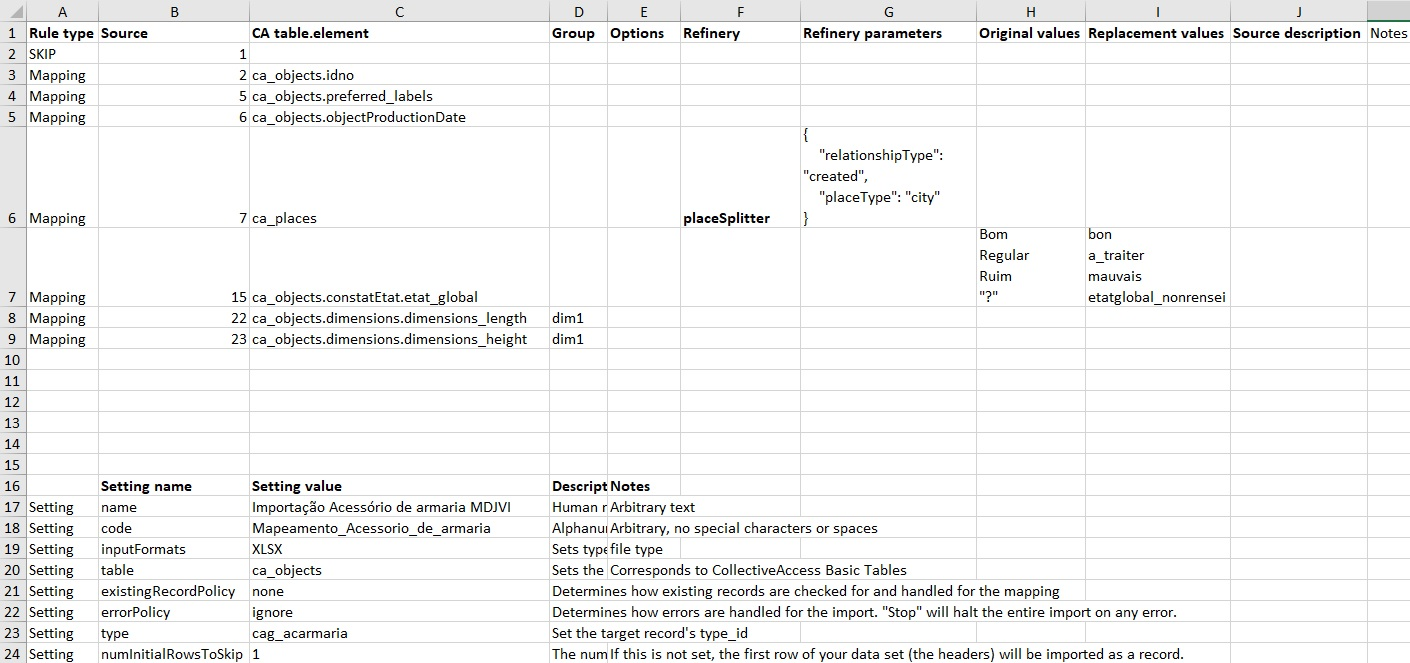
\includegraphics[width=15cm, left]{figuras/ex_map.jpg}
	\caption{Exemplo de arquivo de mapeamento} \label{fig:map}
\end{figure}

Na figura \ref{fig:map} podemos ver um exemplo de um arquivo de mapeamento. Nas linhas 1 a 9 foram definidos os campos que serão importados e seus respectivos destinos nos campos dos objetos configurados no perfil de instalação. É possível perceber o uso de algumas configurações como o agrupamento das dimensões em um único conjunto, o refinamento da importação de lugar, informando que o dado importado é uma cidade e é o local de criação do objeto, e a substituição dos dados de estado de conservação do objeto pelos seus respectivos códigos na lista criada com este objetivo.

Já nas linhas 16 a 24 são definidas as configurações do mapeamento conforme já explicado anteriormente.

\section{Importação dos dados}

\FloatBarrier
Antes de se importar os dados, assim como qualquer modificação grande em banco de dados, é importante criar uma cópia de segurança dos arquivos para evitar perdas e problemas nos objetos importados, principalmente se for a primeira vez que um mapeamento é utilizado.

O Collective Access aceita vários tipos de formato de dados para importação, desde arquivos de Excel em .xls ou .xlsx, provenientes de bancos de dados MYSQL, vários formatos de XML diferentes oriundos de outros SGC como PastPerfect XML e Omeka, de um outro sistema Collective Access, para migrações de um sistema para outro, e até de sistemas web como ULAN e Worldcat. Este projeto utilizou somente os dados já existentes do Museu D. João VI que foi dividido em planilhas de Excel por classe.

Após o tratamento do acervo e a criação de todos os arquivos de mapeamento, a próxima etapa é realizar a importação dos dados. O Providence conta com uma interface fácil e intuitiva, onde primeiro o arquivo de mapeamento é carregado para o site e posteriormente se seleciona o arquivo com os dados a serem importados com o mapeamento selecionado.


\begin{figure}[!ht]{17cm}
	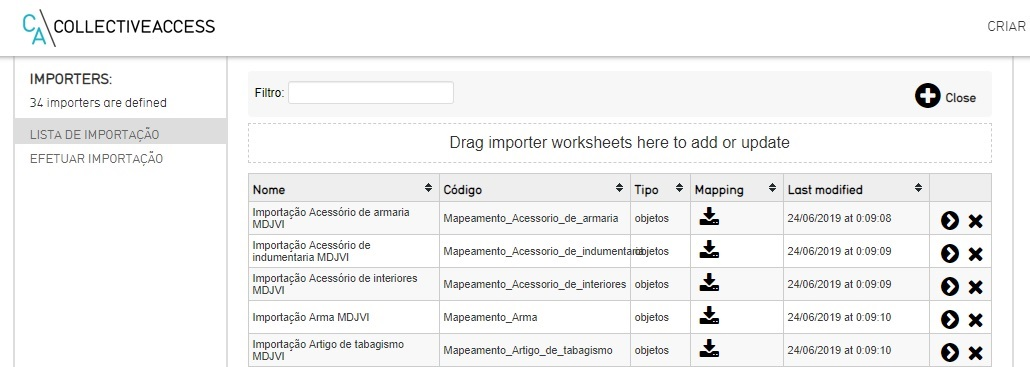
\includegraphics[width=15cm, left]{figuras/tela_map.jpg}
	\caption{Tela de Importação - Mapeamento} \label{fig:mapeamento}
\end{figure}


Na figura \ref{fig:mapeamento} podemos ver a tela onde se carrega o importador com o mapeamento. Pode-se verificar de forma fácil quais mapeamentos já foram enviados para o site e selecionar qual será usado para realizar a importação. Caso se envie uma planilha com um código de mapeamento já utilizado, o site irá substituir a versão antiga pela enviada.

\begin{figure}[!ht]{17cm}
	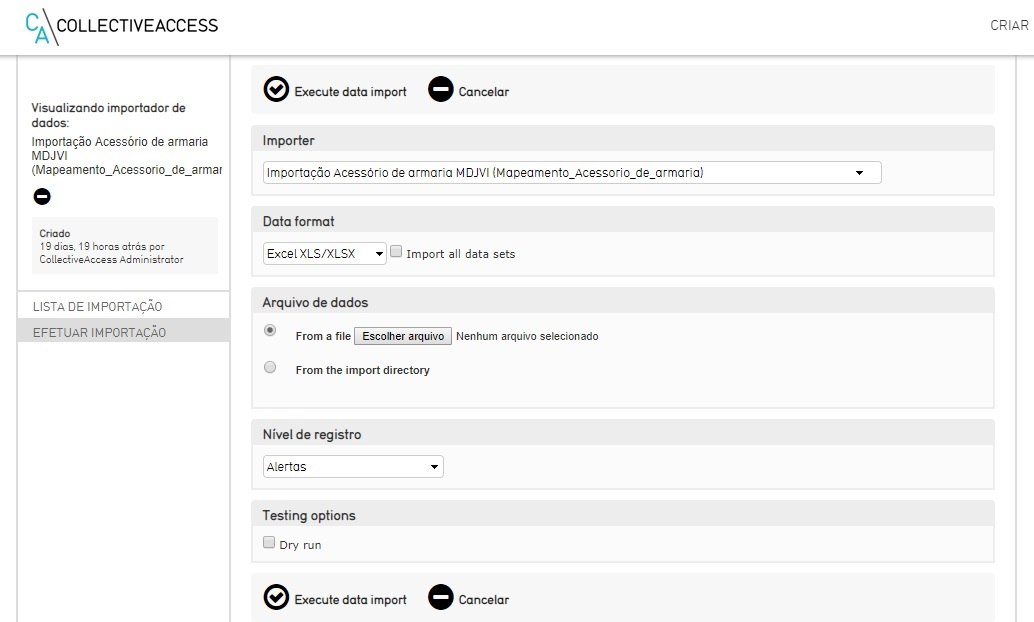
\includegraphics[width=15cm, left]{figuras/tela_imp.jpg}
	\caption{Tela de Importação - Configurações} \label{fig:import}
\end{figure}

Já na figura \ref{fig:import} vemos as definições necessárias antes de se realizar a importação. É necessário informar qual o formato do arquivo que será importado, carregar o mesmo para o site ou, caso ele esteja no diretório de importação, selecionar esta opção. Também é possível escolher o nível de registro que será gravado durante a importação, o que é útil em testes de mapeamento, ou até mesmo realizar uma importação "a seco", que é uma importação de teste onde os dados não são gravados no banco de dados.

Após a importação dos dados, o site irá informar quantos registros foram importados e se ocorreu algum erro. É possível verificar no log da importação, um arquivo gerado automaticamente pelo site, as mensagens de alertas e erros conforme configurado no menu "Nível de Registro" na figura \ref{fig:import}.

\section{Tradução do Providence}

Os arquivos do Collective Access utilizam, por padrão, a língua inglesa. Apesar de se poder trocar o idioma antes ou após a instalação para português brasileiro, a tradução não está completa e, em muitos casos, está errada ou em português de Portugal.

Apesar dos objetos, listas e interfaces já terem sido traduzidos no perfil de instalação, a maior parte do gerenciamento do site e acervo, configuração e importação utiliza dados e informações provenientes de arquivos que o perfil não afeta.

O Collective Access utiliza o sistema \textit{GNU GetText} para gerenciar as traduções dos textos da interface do usuário, armazenando ambas a versão original em inglês e a tradução em um arquivo editável messages.po. Cada tradução é armazenada em uma pasta no diretório app/locale, utilizando o código do idioma traduzido como nome da pasta.

Para um melhor uso dos usuários do site, que podem não ter fluência em inglês, foi utilizado o programa \textit{Poedit} para edição do arquivo com a tradução em português brasileiro. Todas as traduções já existentes foram verificadas e revisadas, e os textos que não continham tradução foram traduzidos. No total foram traduzidos 6444 textos, que podem ser desde uma palavra até parágrafos inteiros.

\section{Painel Inicial do Providence}

Com os dados importados é possível utilizar o Providence para gerenciar todas as funções do Museu. Na tela inicial existe um painel onde é possível adicionar \textit{widgets}, que são pequenas aplicações com diferentes funcionalidades para criar uma interface de sistema de monitoração e gerenciamento personalizado conforme a necessidade do Museu.

Os seguintes \textit{Widgets} já estão disponíveis na instalação do Collective Access:

\begin{itemize}
	\item \textbf{Formulário de pesquisa avançada} - Adiciona um formulário de pesquisa avançada para utilização no painel do site;
	\item \textbf{Relógio} - Adiciona um relógio com o horário atual;
	\item \textbf{Contadores} - Mostra a quantidade total de todos os itens do Collective Access;
	\item \textbf{Acessos recentes} - Exibe os acessos recentes de usuários ao sistema;
	\item \textbf{Links} - Exibe os links do projeto Collective Access.
	\item \textbf{lol Katz} - Mostra uma imagem aleatória de humor;
	\item \textbf{Mensagem do dia} - Exibe a mensagem do dia, que pode ser editada pelo usuário;
	\item \textbf{Caixa de notificação} - Mostra as notificações;
	\item \textbf{Objeto Aleatório} - Exibe um objeto aleatório da coleção;
	\item \textbf{Alterações recentes} - Lista as alterações recentes feitas em objetos ou outros itens;
	\item \textbf{Comentários} - Lista os comentários recentes realizados nos objetos;
	\item \textbf{Registrações} - Lista os últimos cadastros de usuários feitos pelo público;
	\item \textbf{Etiquetas} - Lista as etiquetas criadas recentemente;
	\item \textbf{Criados recentemente} - Exibe os objetos e outros itens criados recentemente;
	\item \textbf{Registros por estado} - Exibe os objetos ou outros itens por estado de catalogação;
	\item \textbf{Gravar pesquisas} - Mostra as pesquisas salvas do painel;
	\item \textbf{Pesquisa por seleção} - Busca por itens nas seleções do usuário;
	\item \textbf{Estado de processamento} - Visualiza o estado atual das tarefas de processamento programadas;
	\item \textbf{Objetos em observação} - Lista os objetos em observação pelo usuário.
\end{itemize}

Além desses \textit{widgets}, é possível criar, configurar e instalar novos conforme a necessidade, bastando colocar os arquivos desenvolvidos no diretório app/widgets do Collective Access, mas para este projeto não houve essa necessidade.

\section{Menu CRIAR}

O primeiro menu do site do Providence é o CRIAR, que deve ser utilizado para a criação de um novo item ou ação relativa ao banco de dados. As seguintes opções aparecem ao se posicionar o mouse sobre este botão:

\begin{itemize}
	\item \textbf{Objeto} - Utilizado para se criar um novo objeto. Deve-se selecionar a categoria entre Acervo Arquivológico e Acervo Museológico, sendo este segundo dividido nas classes e subclasses já citadas;
	\item \textbf{Entidade} - Cria uma entidade, que pode ser uma Família, Organização ou Pessoa Física;
	\item \textbf{Lugar} - Cria um novo lugar, onde posteriormente será selecionado o tipo, como País, Estado ou Cidade. Locais de armazenamento não devem ser criados neste menu;
	\item \textbf{Coleção} - 
\end{itemize}


%================================================================
\chapter{Pawtucket}
%================================================================

%================================================================
\chapter*{Conclusão}
%================================================================

Texto da conclusão.

%\index{Introdução!Capítulo}.

%XXXXXXXXXXXXXXXXXXXXXXXXXXXXXXXXXXXXXXXXXXXXXXXXXXXXXXXXXXXXXXXX
% ELEMENTOS POS-TEXTUAIS
%XXXXXXXXXXXXXXXXXXXXXXXXXXXXXXXXXXXXXXXXXXXXXXXXXXXXXXXXXXXXXXXX
\backmatter % inicia a área dos elementos pós-textuais
%XXXXXXXXXXXXXXXXXXXXXXXXXXXXXXXXXXXXXXXXXXXXXXXXXXXXXXXXXXXXXXXX

%===========================================================
% Referencias via BibTeX
%===========================================================

\citeoption{abnt-options4}
\bibliography{abnt-options4,bibliografia}

%===========================================================
\postextualchapter*{Glossário} % elemento opcional
%===========================================================

\definicao{termo 1}{significado}
\definicao{termo 2}{significado}
\definicao{termo 3}{significado}

%XXXXXXXXXXXXXXXXXXXXXXXXXXXXXXXXXXXXXXXXXXXXXXXXXXXXXXXXXXX
% Apêndices (opcionais)
%XXXXXXXXXXXXXXXXXXXXXXXXXXXXXXXXXXXXXXXXXXXXXXXXXXXXXXXXXXX
\appendix % inicia os apêndices
%XXXXXXXXXXXXXXXXXXXXXXXXXXXXXXXXXXXXXXXXXXXXXXXXXXXXXXXXXXX

%===========================================================

%===========================================================
\postextualchapter{Projeto Original}

\section{Introdução}
O \textbf{Museu D. João VI da Escola de Belas Artes da Universidade Federal do Rio de Janeiro} foi criado em 1979 com a finalidade de preservar a memória do ensino artístico oficial e de fomentar o estudo e a pesquisa da História da Arte Brasileira. Ele vem responder a necessidade da criação de um espaço institucional de preservação do patrimônio e memória do ensino de arte, reunindo a produção da Academia Imperial de Belas Artes, da Escola Nacional de Belas Artes e parte da história recente da Escola de Belas Artes.

O Museu abriga dois acervos distintos, um de obras de arte e outro de documentos, fontes primárias indispensáveis para o desenvolvimento de estudos e projetos de pesquisa em arte, quer no campo teórico quer no aplicado. Estes acervos são o resultado do patrimônio acadêmico produzido pela Escola no período compreendido, principalmente, entre 1820 e 1920.

Com o objetivo de implementar a atividade de pesquisa foi desenvolvido um projeto integrado - Museu D. João VI e Mestrado em História da Arte - EBA/UFRJ, financiado pelo CNPq, que tratou de realizar o inventário científico e sistemático destes dois acervos. 

O processo de sistematização culminou com a sua informatização, por meio de um convênio com o Núcleo de Computação Eletrônica da UFRJ, sendo o Núcleo responsável pela montagem global do sistema.

O trabalho de catalogação e sistematização foi elaborado de forma o mais técnica e criteriosa possível, sendo aplicados inúmeros instrumentos nas suas diversas etapas de identificação e de realização dos inventários. A descrição destes instrumentos, as metodologias aplicadas e os critérios de seleção e ordenação dos acervos são apresentados a seguir, se constituindo em documento técnico imprescindível, não só para o entendimento do processo, assim como para a ampliação da base do banco de dados.

\section{ACERVO MUSEOLÓGICO}
O acervo de obras do \textbf{Museu D. João VI (MDJVI)} tem uma importância singular seja para o estudo e o entendimento da história da formação artística no país, seja para a construção de uma história da arte brasileira. O acervo original da Academia Imperial de Belas Artes tem sua origem na contratação da \textbf{Missão Artística Francesa}, que chegando ao Brasil trouxe na bagagem uma coleção de 42 obras de artistas franceses e italianos, inaugurando a pinacoteca da antiga Academia. Soma-se ainda um número significativo de moldagens de gesso destinadas ao Curso de Escultura, servindo até hoje como material didático. 

Outras coleções foram sendo incorporadas à Academia e à Escola de Belas Artes, tais como as coleções de gravuras holandesas e francesas. Além destas encontra-se uma extensa coleção de medalhas produzidas pelo antigo Curso de Gravura de medalhas e pedras preciosas e, uma importante coleção de desenhos, formada pelos trabalhos de alunos e professores, compreendendo os Cursos de Desenho artístico, Modelo vivo e Desenho arquitetônico. O acervo se caracteriza por reunir um volume considerável de obras-documento, apresentadas nos concursos para professor, como aquelas referentes aos concursos para Prêmio de viagem. Destacam-se, ainda, inúmeras obras selecionadas e premiadas nas exposições oficiais da Academia, entre elas as \textit{Exposições Gerais de Belas Artes} (Salão).

O trabalho de sistematização do acervo museológico compreendeu duas etapas: a realização do inventário completo, com a identificação e fichamento das obras, e a informatização e criação do banco de dados.

Na primeira etapa foi feito um levantamento minucioso da fonte primária, que compreende o acervo completo de artes visuais - desenhos, gravuras, esculturas e pinturas - tomando como base o \textbf{Livro de Tombo do Museu D. João VI} Este processo incluiu a revisão completa das peças já inventariadas, chamando a atenção para duas coleções não museológicas registradas no \textbf{Livro de Tombo}, que são: diplomas e fotografias.

Para a etapa de informatização deste \textbf{Inventário Geral} foi elaborada uma ficha de registro de obras de acordo com as normas técnicas atuais, partindo de dados básicos e universais no que concerne à coleção de artes visuais, apresentando os seguintes campos, distribuídos em duas categorias de informação: dados gerais e dados complementares.

\subsection{Dados Gerais}
\subsubsection{Número de registro}
É o \textbf{número de registro de tombamento}. A numeração respeitou parcialmente o sistema numérico do \textbf{Livro de Tombo} encontrado, seguindo portanto, a sequência natural do número de ordem deste livro, cuja última peça fora registrada sob o número \textbf{2140}. A primeira peça sem registro a ser inventariada recebeu, consequentemente, o número 2141.Para tornar o sistema de numeração mais objetivo, optou-se por manter somente o número de ordem, abandonando o modelo tripartido do livro de tombo original, ou seja, omitindo- se os dígitos referentes ao ano de entrada da peça e à sua categoria. Para as peças compostas de diversas partes adotou-se o uso do complemento alfabético: 
\begin{itemize}
	\item registro \textbf{1463 A} - Classe Objetos pessoais, Subclasse Objetos de adorno, Relógio - e 
	\item registro \textbf{1463 B} - Classe Objetos pessoais, Subclasse Objetos de
	adorno, Estojo.
\end{itemize}

\subsubsection{Classe e Subclasse}
Os conceitos de classe e subclasse adotados foram baseados no ``\textit{Thesaurus para Acervos Museológicos}'' - Fundação Pró-Memória/1987, utilizado, na atualidade, por inúmeros museus brasileiros. De acordo com este sistema a classificação obedece a um único critério, o da funcionalidade original da peça, abolindo-se as classificações antigas, que combinavam a função com materiais e categorias. 

No caso específico do \textbf{MDJVI} a classe predominante no acervo é \textbf{Artes visuais} com suas respectivas sub-classes: 
\begin{itemize}
	\item Construção artística, 
	\item Desenho, 
	\item Desenho arquitetônico, 
	\item Escultura, 
	\item Gravura e 
	\item Pintura.
\end{itemize} 

As outras classes e sub-classes foram também empregadas, mas com menos frequência em função da própria especificidade do acervo em questão que são elas, classes: 
\begin{itemize}
	\item Amostras/fragmentos, 
	\item Caça/guerra, 
	\item Comunicação, 
	\item Construção, 
	\item Embalagem/recipientes, 
	\item Insígnia, 
	\item Interiores, 
	\item Lazer/desporto,
	\item Medição/registro/observação/processamento, 
	\item Objetos cerimoniais, 
	\item Objetos pessoais e 
	\item Trabalho.
\end{itemize} 

Como norma ortográfica para as Classe e Subclasses
estipulou-se o uso de maiúscula somente na primeira letra das nomenclaturas: \textit{Classe - Artes visuais, Subclasse - Desenho arquitetônico.}

As coleções de diploma e fotografia constituíram-se em caso especial pois foram registradas no \textbf{Livro de Tombo do Museu D. João VI}, segundo a classificação prevista no \textit{Thesaurus para acervos museológicos} que prevê o uso da classe \textbf{Comunicação} para os objetos usados para transmitir informações aos seres humanos\footnote{FERREZ Helena Dodd e BIANCHINI, Maria Helena S. \textit{Thesaurus para acervos museológicos}. p. 7.}, e a subclasse \textbf{Documento} para documentos textuais, cartográficos e iconográficos. Constituindo-se, seu uso, caso específico para museus que não possuem setor técnico para tratamento deste tipo de acervo. Baseado nesta particularidade, optou-se pela continuidade do registro estabelecendo-se adaptações para o preenchimento dos campos da ficha de registro. Como norma técnica para este campo, utilizou-se o \textit{Termo} ou \textit{Nome do objeto} junto à subclasse para evitar dúvidas quanto ao acervo consultado, criando-se as classificações: \textit{Comunicação - Documento diploma e Comunicação - Documento fotográfico}.


\subsubsection{Autoria}
Campo destinado ao registro de pessoa física ou jurídica que concebeu material e/ou intelectualmente a obra, acompanhado de cronologia. O autor foi situado cronologicamente tendo como referência os \textbf{anos de nascimento e morte}, com informações coletadas do \textit{Dicionário das Artes Plásticas no Brasil}, \textit{Dicionário Brasileiro de Artistas Plásticos} e \textit{Dictionnaire des Peintres, Sculpteurs, Dessinateurs et Graveurs}, citados em referência bibliográfica do projeto em questão. Para a normatização dos dados estipulou-se:

\begin{itemize}
	\item para entrada de dados no campo registrar-se em maiúscula o último sobrenome do autor, seguido de vírgula, do prenome ou prenomes em minúscula, e dos anos de nascimento e morte entre parênteses.
	\item para o caso de autores não identificados registrar-se no campo, não identificada;
	\item para pseudônimos registrá-los entre aspas, precedidos do autor e dos anos de nascimento e morte entre parênteses;
	\item para a coleção de diplomas registrar-se a instituição ou órgão gerador do documento em maiúsculas;
	\item para a coleção de gravuras registrar-se o autor que elaborou a matriz com o último sobrenome em maiúscula seguido de vírgula, do prenome ou prenomes em minúscula e os anos de nascimento e morte entre parênteses.
\end{itemize}

\subsubsection{Assinatura}
Destina-se ao registro do local da assinatura do autor na obra. A informação sobre a localização da assinatura na obra seguiu as normas do \textit{Manual de Catalogação de Pinturas, Esculturas, Desenhos e Gravuras}, publicado pelo \textbf{Museu Nacional de Belas Artes}. Listagem em anexo.

\subsubsection{Co-autoria}
Identifica os demais autores envolvidos na criação da obra, especificamente para as subclasses de \textbf{gravura} e \textbf{diploma}. A normatização criada estabelece:
\begin{itemize}
	\item a inserção do último sobrenome do autor em caixa alta seguido de vírgula e do prenome ou prenomes em caixa baixa, sem acrescentar anos de nascimento e morte;
	\item a sequência de inscrição: nome do premiado e autor do desenho do diploma, de acordo com a norma anterior, para a coleção de diplomas;
	\item o registro do local de assinatura na obra dos respectivos autores em espaço designado no campo.
\end{itemize}

\subsubsection{Título}
Os títulos foram extraídos de dois tipos de fontes: 
\begin{description}
	\item[fonte primária ] transcrição da própria obra;  
	\item[fonte secundária] por atribuição de especialista e de catalogador, fundamentados em pesquisa iconográfica tendo como referência bibliografia especializada.
\end{description}

Grande parte das obras do acervo do MDJVI não apresentam títulos pois compõe os conjuntos de material didático, exercícios de aulas e provas de concursos. Sendo assim a inúmeros títulos foi aplicado o critério de atribuição, adotando-se para a identificação da obra a forma mais simples e direta - \textbf{identificação do tema} ou da própria imagem, acrescidas informações complementares pertinentes, de modo a dar mais clareza ao processo de identificação.

Esta informações complementares seguem os seguintes critérios:
\begin{itemize}
	\item as cópias de obras primas famosas receberam os mesmos títulos pelos quais são conhecidos, seguidos da observação entre parênteses - (\textit{cópia de...}), exemplos:\\ 
	Vênus Anadiomene (\textit{cópia de Lisipo}), \\
	Hércules Farnese (\textit{cópia de Praxíteles}), \\
	Napoleão em Jafa (\textit{cópia de Gros}).
	\item os temas mitológicos, históricos e religiosos, claramente reconhecidos pela sua representação ou pelos atributos utilizados pelos personagens receberam os títulos convencionais, tais como: \textit{Sansão e Dalila}, \textit{Moisés}, \textit{Pigmalião e Galatéia}, \textit{A morte de Sócrates}, \textit{A crucificação de Cristo}.
	\item representações do nu apresentam no título o complemento a que se refere sua técnica de representação acadêmica: \textit{Nu feminino (academia)}, \textit{Nu feminino (academia - 2 esboços)}.
	\item em determinadas obras foi acrescido ao título atribuído notas extraídas da própria obra mas que sozinhas não determinavam seu conteúdo: \textit{Busto feminino - ``grand étude aux deux crayons n. 44''}.
	\item cópias de detalhes arquitetônicos de construção de monumentos renomados ou ainda aquelas identificadas no suporte pelo próprio autor: \textit{Medalhão da portada da igreja do Carmo (cópia de Aleijadinho, São João del Rei)}.
	\item na \textbf{Subclasse Escultura} devido a grande quantidade de cópias do período clássico foi utilizado o recurso de identificação complementar registrando-se o tipo e o período: \textit{Ângulo de capitel - alto relevo (arte gótica)}, \textit{Antefixo (arte grega)}.
	\item na \textbf{Subclasse Desenho} as cópias de esculturas foram identificadas também de forma complementar: \textit{``São Tiago'' (cópia de escultura)}, \textit{Atleta grego (cópia de escultura)}.
	\item na \textbf{Subclasse Documento diploma} o campo \textbf{Título} foi preenchido com o nome da pessoa premiada encabeçado pela nomenclatura Diploma: Diploma de João Gelabert de Simas.
\end{itemize}

Como norma ortográfica foi definido que somente os títulos e informações complementares extraídos de fonte primária entrariam entre aspas, sendo regra geral para todos os títulos a inscrição da primeira letra em maiúscula e as demais minúsculas, salvo nomes de cidades, acidentes geográficos, pessoas e correlatos, exemplos: ``\textit{Interior de um rancho}'', ``\textit{Igreja matriz da vila de Aquiras}'', Vista da matriz e do Santo Cruzeiro - Ceará, Flor, Serra do Boqueirão de Lavras, Busto feminino - ``grand étude aux deux crayons n.44''.

\subsubsection{Data}
Campo destinado ao registro da data de execução da obra. Procurou-se não deixar o item datação sem uma referência, se determinando, quando possível, década, ano e século. O processo de preenchimento deste campo foi realizado se extraindo a informação da própria obra, muitas vezes com a utilização de lentes de aumento e recursos técnicos apropriados: outras vezes a partir de pesquisa iconográfica tomando-se como base a produção do autor, pois que inúmeras obras referem-se a trabalhos realizados em épocas específicas da formação deste, destacando-se as premiações acadêmicas (Medalha de ouro, Medalha de Prata, Menção honrosa), os Prêmios de viagem ao exterior, os envios de Pensionistas, exposições oficiais, salões, concursos para magistério, encomendas oficiais; por confrontação foi atribuído o período de execução. Outra fonte utilizada para o preenchimento deste campo foram as biografias.

A inscrição dos dígitos referentes a data foi feita considerando a não identificação da década - \textbf{18\_\_}, a não identificação do ano: \textbf{195\_} e nos trabalhos onde não foi possível nenhuma forma criteriosa de identificação adotou-se a indicação \textit{s/d (sem data)} para evitar atribuições disparatadas.

\subsubsection{Local}
Campo destinado ao registro preciso do local onde a obra foi executada, sendo a informação extraída da própria obra. Como norma de inserção de dados estipulou-se o uso de maiúscula na primeira letra da informação.

\subsubsection{Técnica/material}
Para o registro dos dados deste campo tomou-se como referência o \textit{Sistema de Informação do Museu Nacional de Belas Artes} ( publicação do Patrimônio Artístico Nacional - 1995). Esta opção fundamentou-se na constatação de características comuns existentes entre os acervos do \textbf{MDJVI} e do \textbf{Museu Nacional de Belas Artes}.

Na aplicação das classificações, para os trabalhos bidimensionais, subclasses \textbf{Desenho}, \textbf{Pintura}, \textbf{Gravura}, \textbf{Documento fotográfico} e D\textbf{ocumento diploma}, especificou-se primeiro o processo e por último o suporte: \textit{sanguínea/papel}, \textit{óleo/tela}, \textit{buril/papel}, \textit{PB/papel}, \textit{semi off-set/papel}.

A classificação da \textbf{Subclasse Escultura} foi feita destacando-se os materiais em primeira ordem, uma vez que a técnica se encontra implícita: \textit{bronze}, \textit{cobre}, \textit{prata}, \textit{marfim}, \textit{madeira}, \textit{mármore}, \textit{resina de poliéster}, \textit{gesso}, \textit{terracota}, \textit{prata e madeira}, \textit{ágata e jade} etc. Como as peças em gesso constituem 80\% da coleção de esculturas, para este material foi também identificada a técnica: \textit{gesso patinado}, \textit{moldagem}, \textit{talha e relevo}.

Para as demais classes, destacou-se os materiais empregados na confecção das peças: \textit{Algodão}, \textit{Algodão acetinado}, \textit{Âmbar}, \textit{Cristal e prata}, \textit{Plumas (papo de cisne)/madrepérola}, \textit{seda e fio de prata}; também apresentando a técnica quando identificada: \textit{Bordado}, \textit{Jato de areia}, \textit{Biscuit}, \textit{Tear jacar} e \textit{Valenciana}. Estipulou-se como norma o registro da primeira letra da informação em maiúscula.

\subsubsection{Dimensões}
A medição de uma obra é realizada para cuidar de sua identificação e
segurança, para o dimensionamento do espaço e da carga exigida para sua exposição, objetivando a sua guarda, a confecção de embalagem e seu transporte.

Para o preenchimento do campo \textbf{Dimensões} foram obedecidas as normas internacionais para obras bidimensionais e tridimensionais, que estipulam a seguinte ordem de entrada dos dados: 
\textit{altura, largura, profundidade,} registradas em centímetros. Para as obras \textbf{circulares} é determinada a medida do diâmetro sendo colocado a seguir do valor a letra ``\textbf{d}'' minúscula entre parênteses - \textbf{(d)} e sua espessura; para as obras \textbf{ovais} são registrados os valores de menor e maior larguras acompanhados pela letra ``\textbf{o}'' entre parênteses \textbf{(o)} e sua espessura.

As dimensões das \textbf{obras emolduradas} e das \textbf{esculturas} com base foram registradas tomando primeiramente só o suporte ou peça e outra acrescida da moldura ou base: obra emoldurada - 55,0 x 46,0 cm - c/baguete: 57,2 x 48,0; escultura com base - 25,0 x 16,0 x 22,0cm - c/base: 35,0 x 28,8 x 17,0 cm. 

Para as \textbf{gravuras} foram registradas as dimensões do suporte e do campo impresso separadamente: 35,3 x 27,0 cm - ci: 21,0 x 14,0 cm. 

Para a entrada destes dados ainda segue-se a norma de entrada da primeira medida seguida de espaço, do sinal \textbf{x}, espaço e entrada da segunda e/ou terceira medidas. Para as peças de \textbf{gravura} destaca-se a dimensão do campo impresso identificando-o como \textbf{ci} seguido de dois pontos e da dimensão inserida com a mesma norma apresentada anteriormente, aplicando-se a mesma norma para obras com base que se identifica c/base, com moldura - c/moldura, com baguete - c/baguete.

\subsubsection{Concursos, Exposições, Premiações, Pensionistas}
Campo destinado ao registro de dados extraídos da própria obra ou coletados em bibliografia pertinente, codificados através de índice que destaca os assuntos que geraram a nomenclatura do campo. Seus dados complementam-se com os do campo \textbf{Observação} que também é destinado aos dados mais específicos que se remetem a este campo. Listagem em anexo.

\subsubsection{Tema}
Registro de termo que descreve o conteúdo temático da obra tendo como referência o \textit{título} e a \textit{imagem}. Utilizado como mais um instrumento de pesquisa, adotado somente para as classes \textbf{Artes visuais} e \textbf{Construção}. Listagem em anexo.

\subsubsection{Localização}
Campo de registro do local determinado onde a peça se encontra no espaço museográfico, alterando-se de acordo com a movimentação da mesma. Para a melhor formatação das informações foram criados códigos de localização (ver anexo).

\subsubsection{Aquisição}
Destinado a registrar o ano e o modo de aquisição da obra.

\subsubsection{Estado de conservação}
Para determinar o estado de conservação da obra foram estipuladas três categorias:
\begin{enumerate}
	\item \textbf{Bom}	- para as obras estáveis e sem grandes problemas;
	\item \textbf{Regular} - para as obras que têm danos passíveis de serem tratados;
	\item \textbf{Ruim} - para as que estão muito danificadas, inclusive, com perda de suporte ou mutiladas, às vezes totalmente fragmentadas.
\end{enumerate}

\subsubsection{Movimentação}
Para registro do histórico de movimentação da obra que eventualmente venham a ocorrer.

\subsubsection{Observações}
Reservado àquelas informações mais específicas da obra e para complementação de dados do campo \textbf{Concursos}, \textbf{Exposições}, \textbf{Premiações}, \textbf{Pensionistas}.
Registra-se neste campo:
\begin{itemize}
	\item \textbf{inscrições} que constam na obra atestando propriedade ou origem da peça no caso das moldagens de gesso, geralmente com plaquetas incrustadas com o nome do museu onde se encontra a obra original que foi reproduzida, e dedicatórias;
	\item detalhamento da forma de \textbf{aquisição} quando pertence à \textit{Coleção Ferreira das Neves}, doada à antiga Escola Nacional de Belas Artes em 1947 pelo colecionador português \textit{Jerônimo Ferreira ads Neves}, registrando-a com as iniciais maiúsculas \textbf{CFN}.
	\item \textbf{número da Exposição geral}; 
	\item \textbf{seção da Exposição geral};
	\item \textbf{número da obra na Exposição};
	\item \textbf{aula} em que o premiado estava matriculado;
	\item \textbf{informações complementares} sobre o tipo de medalha;
	\item \textbf{identificação} do trabalho do autor do desenho do diploma;
	\item \textbf{transcrição}, no caso das gravuras que possuem mais de um autor, das funções que cada autor desempenhou na elaboração da obra;
	\item \textbf{dúvidas}.
\end{itemize}


\subsubsection{Relatórios técnicos}
Como etapa do desenvolvimento do projeto, e de consequente uso do \textit{programa Access} constatou-se a necessidade de criação de relatórios técnicos parciais para consulta do acervo. Constituem-se em relatórios básicos que concentram dados relativos às atividades técnicas da área de Museologia como: a catalogação que é uma análise de maior profundidade que identifica e relaciona os bens culturais através de estudo; a conservação que consiste em tratamento preventivo à restauração; curadoria que trata da disposição do acervo para o público; e a restauração que é a intervenção técnica para reabilitação da obra. 

Para elaboração de tais relatórios foram combinados campos da ficha de registro para construir informações significativas que atendem às atividades técnicas gerais determinadas.
\begin{itemize}
	\item Autoria, Co-autoría, Título, Concursos, Exposições, Pensionistas, Observação;
	\item Conservação, Data, Técnica/material, Localização;
	\item Conservação, Técnica/material, Dimensões, Localização;
	\item Conservação, Técnica/material, Localização;
	\item Conservação, Técnica/material, Observação, Localização;
	\item Subclasse, Autoria, Co-autoria, Titulo, Data;
	\item Tema, Autoria, Co-autoria, Concursos, Observação.
\end{itemize}


\section{ANEXOS DO ACERVO MUSEOLÓGICO}
\subsection{Classes/Subclasses}
\begin{itemize}
	\item Amostras/Fragmentos
	\item Artes visuais
	\begin{itemize}
		\item Construção artística
		\item Desenho
		\item Desenho arquitetônico
		\item Escultura
		\item Gravura
		\item Pintura
	\end{itemize}
	\item Caça/Guerra 
	\begin{itemize}
		\item Acessório de armaria
		\item Arma
	\end{itemize}
    \item Comunicação
    \begin{itemize}
    	\item Documento diploma
    	\item Documento fotográfico
    \end{itemize}
	\item Construção
	\begin{itemize}
		\item Fragmento de construção
	\end{itemize}
	\item Embalagens/Recipientes
	\item Insígnia
	\begin{itemize}
		\item Bandeira
	\end{itemize}
	\item Interiores
	\begin{itemize}
		\item Acessório de interiores
		\item Objeto de iluminação
		\item Peça de mobiliário 
		\item Utensílio de cozinha/mesa
	\end{itemize}
	\item Lazer/Desporto
	\item Medição/Registro/Observação/Processamento
	\begin{itemize}
		\item Instrumento de precisão/ótico
	\end{itemize}
	\item Objetos cerimoniais
	\begin{itemize}
		\item Objeto comemorativo
		\item Objeto de culto
		\item Panegírico
	\end{itemize}
	\item Objetos pessoais
	\begin{itemize}
		\item Acessório de indumentária
		\item Artigo de tabagismo
		\item Artigo de toalete
		\item Objeto de adorno
		\item Objeto de auxílio/conforto pessoais
		\item Objeto de devoção pessoal
		\item Peça de indumentária
	\end{itemize}
	\item Trabalho
	\begin{itemize}
		\item Equipamento de artistas/artesãos
		\item Equipamento de comunicação escrita
		\item Equipamento de fiação/tecelagem
		\item Instrumento musical
	\end{itemize}
\end{itemize}

\subsection{Abreviaturas de localização de assinaturas nas obras}
  	 \begin{tabbing}
  	 	\hspace{0.7cm}\=\hspace{8cm}\=\hspace{1cm}\=\kill
  	 c	\> - centro \> vc \> - verso centro \\ 
  	 cd	\> - centro à direita \> vcd \> - verso centro direita\\ 
  	 ce	\> - centro à esquerda \> vce \> - verso centro à esquerda\\
  	 cid\> - canto inferior direito\> vcid \> - verso canto inferior direito\\ 
  	 cie\> - canto inferior esquerdo \> vcie \> - verso canto inferior esquerdo\\ 
  	 csd\> - canto superior direito \> vcsd \> - verso canto superior direito\\
  	 cse\> - canto superior esquerdo \> vcse \> - verso canto superior esquerdo\\ 
  	 ebc\> - embaixo no centro \> vebc \> - verso embaixo no centro\\ 
  	 ebd\> - embaixo à direita \> vebd \> - verso embaixo à direita\\
  	 ebe\> - embaixo à esquerda\> vebe \> - verso embaixo à esquerda\\ 
  	 ecc\> - em cima no centro \> vecc \> - verso em cima no centro\\ 
  	 ecd\> - em cima à direita \> vecd \> - verso em cima à direita\\ 
  	 ece\> - em cima à esquerda \> vece \> - verso em cima à esquerda
  	 \end{tabbing} 	
 	
\subsection{Temas}

\begin{tabbing}
	\hspace{8,7cm}\=\hspace{1cm}\=\kill
	Abstrato \> Figura Humana \\ 
	Alegórico	\> Funerário\\ 
	Anatômico \> Gênero\\
	Animalista \> Heráldico\\
	Arquitetura \> Histórico \\ 
	Caricatural	\> Literário\\ 
	Cenografia \> Marinha\\
	Composição geométrica \> Mitológico\\
	Decoração \> Natureza morta \\ 
	Documental	\> Nu\\ 
	Elemento arquitetônico \> Outros\\
	Elemento arquitetônico-fragmento (para  \> Paisagem\\   
	capitéis e talha de igreja) \> Religioso\\
	Elemento arquitetônico-estudo (para  \> Retrato\\   
	cópias de gesso) \> Social\\
	Estudo de composição  \> \\
\end{tabbing}

\subsection{Técnicas e materiais}

\begin{tabbing}
	\hspace{8,7cm}\=\hspace{1cm}\=\kill
	\textbf{A} \>  \\ 
	Aço e bronze dourado	\> Água tinta, água forte e relevo/papel\\ 
	Acrílica/eucatex \> Água tinta, buril e ponta seca/papel\\
	Acrílica/madeira \> Água tinta/papel\\
	Acrílica/tela  \> Aguada de nanquim/papel\\ 
	Ágata \> Aguada de sépia/papel \\ 
	Ágata/jade	\> Aguada, aquarela e giz/papel\\ 
	Água forte e água tinta/papel \> Algodão\\
	Água forte, água tinta e ponta seca/papel \> Algodão acetinado \\
	Água forte, verniz mole e relevo/papel \> Âmbar \\ 
	Água forte/papel	\> Aquarela e lápis de cor/papel\\ 
	Água tinta e água forte/papel \> Aquarela e pastel/papel\\
	Água tinta, água forte e ponta seca/papel  \> Aquarela/papel\\	   
\end{tabbing}

\begin{tabbing}
	\hspace{8,7cm}\=\hspace{1cm}\=\kill
	\textbf{B} \>  \\ 
	Bico de pena e talha/marfim	\> prata e lantejoula\\
	Biscuit \> Bordado/tecido, seda, ouro e prata\\
	Bordado/contas pretas \> Bordado/veludo e fio metálico\\
	Bordado/couro, pelica, seda, fio de ouro e \> Bronze\\ 
	prata \>  Bronze dourado/madeira\\ 
	Bordado/linha de seda e linho \> Bronze dourado/mármore\\ 
	Bordado/seda \> Bronze/cerâmica\\
	Bordado/seda, fio de ouro e galão \> Bronze/madeira \\
	Bordado/seda, fio de ouro e prata \> Bronze/mármore \\ 
	Bordado/seda, fio de ouro, prata e bordado	\> Bronze/pedra \\ 
	Bordado/seda, franja, fio de ouro e \> Buril e água forte/papel\\
	lantejoulas  \> Buril e ponta seca/papel\\
	Bordado/tafetá, fio de ouro e prata  \> Buril e têmpera/papel\\
	Bordado/tecido, seda, fio de ouro,  \> Buril/papel\\	   
\end{tabbing}

\begin{tabbing}
	\hspace{8,7cm}\=\hspace{1cm}\=\kill
	\textbf{C} \>  \\ 
	Cabelo trançado/metal dourado	\> Cobre\\
	Carvão \> Contas, vidro e metal\\
	Carvão e crayon/papel \> Cópia fotostática/papel\\
	Carvão e giz/papel \> Couro lavrado/madeira e metal\\ 
	Carvão e grafite/papel \>  Couro, cetim e madeira\\ 
	Carvão e sanguínea/papel \> Couro, veludo e seda\\ 
	Carvão, crayon e giz/papel \> Crayon e aquarela/papel\\
	Carvão, crayon e grafite/papel \> Crayon e carvão/papel \\
	Carvão, crayon e pastel/papel \> Crayon e giz branco/papel \\ 
	Carvão, crayon e sanguínea/papel \> Crayon e giz/papel \\ 
	Carvão, crayon e sépia/papel \> Crayon e grafite/papel\\
	Carvão, crayon, sanguínea e giz/papel  \> Crayon e pastel/papel\\
	Carvão, giz e crayon/papel  \> Crayon e sanguínea/papel\\
	Carvão, giz e grafite/papel  \> Crayon e sépia/papel\\
	Carvão, giz e sanguínea/papel \> Crayon, carvão e giz/papel\\
	Carvão, giz e sépia/papel \> Crayon, carvão e sanguínea/papel\\
	Carvão, grafite e aquarela/papel \> Crayon, carvão, sanguínea e giz/papel\\
	Carvão, pastel e giz/papel \> Crayon, giz e grafite/papel\\ 
	Carvão, sanguínea e giz/papel \>  Crayon, giz e sanguínea/papel\\ 
	Carvão/papel \> Crayon, pastel e carvão/papel\\ 
	Carvão/tela \> Crayon, sanguínea e pastel/papel\\
	Cerâmica \> Crayon/papel \\
	Chumbo e mármore \> Cristal \\ 
	Chumbo e pedras sintéticas	\> Cristal e prata (tampa) \\	   
\end{tabbing}

\begin{tabbing}
	\hspace{8,7cm}\=\hspace{1cm}\=\kill
	\textbf{E} \>  \\ 
	Ébano, marfim e prata	\> Esmalte/metal\\
	Encáustica/cartão \> Esmalte/prata\\
	Esmalte \> \\	   
\end{tabbing}

\begin{tabbing}
	\hspace{8,7cm}\=\hspace{1cm}\=\kill
	\textbf{F} \>  \\ 
	Faiança	\> Folha de Flandres\\
	Ferro \> Folha de Flandres/couro\\
	Fio de seda pura/passamanaria \> Fotolitografia/papel \\	
	Fio de seda/adamascado \> Fotopintura/tela\\   
\end{tabbing}

\begin{tabbing}
	\hspace{8,7cm}\=\hspace{1cm}\=\kill
	\textbf{G} \>  \\ 
	Gesso	\> Grafite e sanguínea/papel\\
	Gesso patinado \> Grafite, crayon e giz/papel\\
	Gesso/madeira \> Grafite, crayon e sanguínea/papel \\	
	Gesso/moldagem \> Grafite, nanquim, aquarela e carvão/papel\\
	Giz, carvão e sanguínea/papel \> Grafite, sanguínea e lápis/papel\\
	Glíptica/ouro e pedra \> Grafite/papel\\
	Glíptica/pedra \> Granito \\	
	Glíptica/pedra e madeira \> Gravura/marfim\\   
	Glíptica/prata e pedra	\> Gravura/marfim e metal dourado\\
	Grafite e aquarela/papel \> Gravura/papel e vidro\\
	Grafite e crayon/papel \> Guache c/ açúcar e relevo/papel \\	
	Grafite e giz/papel \> Guache e aquarela/papel\\ 
	Grafite e lápis/papel \> Guache/marfim, chifre, couro, metal e vidro \\	
	Grafite e nanquim/papel \> Guache/marfim, ouro e chifre\\      
\end{tabbing}

\begin{tabbing}
	\hspace{8,7cm}\=\hspace{1cm}\=\kill
	\textbf{H} \>  \\ 
	Heliogravura/papel	\> \\   
\end{tabbing}

\begin{tabbing}
	\hspace{8,7cm}\=\hspace{1cm}\=\kill
	\textbf{I} \>  \\ 
	Impressão e lápis de cor/papel \> Impressão/seda\\ 
	Impressão/papel \> Incrustado/ouro e tartaruga \\	
	Impressão/papel, tecido e madeira \> \\    
\end{tabbing}

\begin{tabbing}
	\hspace{8,7cm}\=\hspace{1cm}\=\kill
	\textbf{J} \>  \\ 
	Jato de areia/cristal	\> \\   
\end{tabbing}

\begin{tabbing}
	\hspace{8,7cm}\=\hspace{1cm}\=\kill
	\textbf{L} \>  \\ 
	Laca e folha de ouro/madeira \> Linho\\ 
	Laca/metal \> Linoleogravura/papel \\
	Lápis de cor e carvão/papel \> Litografia a vapor/papel\\ 
	Lápis de cor/tecido \> Litografia/papel \\	
	Linha enrolada com fio metálico \> \\    
\end{tabbing}

\begin{tabbing}
	\hspace{8,7cm}\=\hspace{1cm}\=\kill
	\textbf{M} \>  \\ 
	Madeira	\> Maneira negra/papel\\
	Madeira (jacarandá) \> Marfim\\
	Madeira e apliques de bronze \> Marfim e veludo \\	
	Madeira e metal \> Marfim/madeira\\
	Madeira e papier maché \> Mármore\\
	Madeira pintada \> Massa acrílica e tinta acrílica/eucatex\\
	Madeira policromada \> Metal \\	
	Madeira vazada e pintada \> Metal dourado\\   
	Madeira, bronze e espelho	\> Metal e técnica mista/papel\\
	Madeira, couro e veludo \> Metal e verniz de álcool/papel\\
	Madeira, couro e veludo roxo \> Metal prateado \\	
	Madeira, mármore e metal dourado \> Metal, água tinta e relevo/papel\\ 
	Madeira, metal e tecido \> Metal, água tinta e verniz mole/papel \\	
	Madeira, metal e veludo \> Metal/esmalte\\
	Madeira, palhinha e bronze dourado \> Metal/madeira \\	
	Madeira/bronze dourado \> Metal/papel\\
	Madeira/gesso \> Metal/vitral\\
	Madeira/metal \> Moldagem/gesso\\
	Madeira/palhinha \> Moldagem/gesso bronzeado \\	
	Madeira/prata \> Moldagem/gesso e madeira\\   
	Madeira/tecido	\> Moldagem/gesso patinado\\
	Madeira/veludo \> Mosaico/mármore amarelo\\
	Madeira/vidro \> Mosaico/mármore preto \\	
	Madrepérola \> Mosaico/metal dourado\\ 
	Madrepérola e metal \> Mosaico/metal e granito \\	
	Maneira de crayon/papel \> \\        
\end{tabbing}

\begin{tabbing}
	\hspace{8,7cm}\=\hspace{1cm}\=\kill
	\textbf{N} \>  \\ 
	Nanquim e aquarela/papel	\> Nanquim e sépia/papel\\
	Nanquim e grafite/papel \> Nanquim e tinta ferrogálica/papel\\
	Nanquim e guache/papel \> Nanquim, grafite e aquarela/papel \\	
	Nanquim e pastel/papel \> Nanquim/papel\\
\end{tabbing}

\begin{tabbing}
	\hspace{8,7cm}\=\hspace{1cm}\=\kill
	\textbf{O} \>  \\ 
	Off-set/papel	\> Óleo/papel e madeira\\
	Óleo e carvão/tela e papelão \> Óleo/tela\\
	Óleo/cartão \> Óleo/tela (marruflagem) \\	
	Óleo/cartão e tela \> Óleo/tela e cartão\\
	Óleo/cobre	\> Óleo/tela e madeira\\
	Óleo/eucatex \> Óleo/tela e papelão\\
	Óleo/madeira \> Ouro, brilhante e platina \\	
	Óleo/marfim \> Ouro, esmalte e pedras preciosas\\
	Óleo/metal \> Ouro, esmalte, vidro e diamante \\	
	Óleo/papel e cartão \> \\
\end{tabbing}

\begin{tabbing}
	\hspace{8,7cm}\=\hspace{1cm}\=\kill
	\textbf{P} \>  \\ 
	Papelão/couro cor grená	\> Pó de pedra\\
	Pastel oleoso/papel \> Ponta seca e água tinta/papel\\
	Pastel/papel \> Ponta seca e roulette/papel \\	
	PB/papel \> Ponta seca, berceau e buril/papel\\
	Pedra	\> Ponta seca/papel\\
	Pedra (basalto)	\> Porcelana\\
	Pedra, massa, fibra vegetal/madeira \> Porcelana branca\\
	Pedra-sabão \> Porcelana/metal dourado e esmalte \\	
	Pintura metálica policromada/cerâmica \> Prata\\
	Pintura/cerâmica	\> Prata e bronze dourado\\
	Pintura/madeira \> Prata e ouro\\
	Pintura/marfim \> Prata, ouro e esmalte \\	
	Pintura/porcelana \> Prata, vidro e esmalte\\
	Pintura/tecido, veludo e pérolas \> Prata/madeira \\	
	Plumas (papo de cisne)/madrepérola \> \\
\end{tabbing}

\begin{tabbing}
	\hspace{8,7cm}\=\hspace{1cm}\=\kill
	\textbf{R} \>  \\ 
	Relevo/gesso	\> Resina e ferro niquelado\\
	Relevo/gesso e madeira \> Resina/gesso\\
	Resina de poliester \>  \\	
\end{tabbing}

\begin{tabbing}
	\hspace{8,7cm}\=\hspace{1cm}\=\kill
	\textbf{S} \>  \\ 
	Sanguínea e carvão/papel	\> Sanguínea/papel\\
	Sanguínea e crayon/papel \> Seda e fio de ouro\\
	Sanguínea e giz/papel	\> Seda e fio de prata\\
	Sanguínea e sépia/papel \> Semi off-set/papel\\
	Sanguínea, carvão e giz/papel	\> Sépia e sanguínea/papel\\
	Sanguínea, crayon e giz/papel \> Sépia/papel\\
	Sanguínea, giz e carvão/papel \> Serigrafia/papel\\
\end{tabbing}

\begin{tabbing}
	\hspace{8,7cm}\=\hspace{1cm}\=\kill
	\textbf{T} \>  \\ 
	Tafetá de seda pura	\> Tecido\\
	Talha e relevo/madeira e metal \> Tecido e fio de ouro\\
	Talha e torneado/madeira	\> Tecido pintado/madeira\\
	Talha/madeira \> Tecido pintado/renda e madeira\\
	Talha/madeira dourada pintada (escaiola)	\> Tecido tingido\\
	Talha/marfim \> Tecido, seda, fio de ouro e fio de prata\\
	Talho doce/papel \> Têmpera/cartão\\
	Tapeçaria/gorgurão de seda bordado	\> Terracota\\
	Tear jacar/fio de seda adamascado \> Terracota/granito\\
	Tear jacar/fio de seda puro \> Tipografia/papel\\
\end{tabbing}

\begin{tabbing}
	\hspace{8,7cm}\=\hspace{1cm}\=\kill
	\textbf{V} \>  \\ 
	Valenciana/linha	\> fibra vegetal/madeira\\
	Vidro \> Vidro/chumbo e ferro\\
	Vidro e bronze dourado	\> Vidro/chumbo, ferro e madeira\\
	Vidro leitoso pintado \> Vidro/cristal\\
	Vidro, cerâmica, pedra, massa e \> Vinílica/tela e madeira\\
\end{tabbing}

\begin{tabbing}
	\hspace{8,7cm}\=\hspace{1cm}\=\kill
	\textbf{X} \>  \\ 
	Xilogravura/papel	\> Xilogravura/papel de arroz\\
\end{tabbing}

\begin{tabbing}
	\hspace{8,7cm}\=\hspace{1cm}\=\kill
	\textbf{Z} \>  \\ 
	Zincografia/papel	\> \\
\end{tabbing}

\section{ACERVO ARQUIVÍSTICO}
\subsection{Diagnóstico}

O acervo, inicialmente, guardado em 8 arquivos e 2 armários de aço, é composto por documentos avulsos e encadernados. Os documentos avulsos achavam-se acondicionados em pastas comuns ou suspensas, ora ordenados alfabeticamente (pasta dos professores e artistas), ora por ordem cronológica (pedidos e matrículas) ou por assunto (obras).

As pastas dos professores/artistas ocupavam dois arquivos e eram formadas por documentos originais e por xerox. Estas tinham por objetivo duplicar o original, quando duas ou mais pessoas eram mencionadas: o original era arquivado em uma das pastas e as reproduções distribuídas pelas pastas das demais pessoas citadas no original. Este procedimento provocou um aumento irreal do acervo.

Quanto a instrumentos de pesquisa, não se obteve qualquer informação sobre a sua existência, ou dos critérios adotados na organização dessa parte do acervo. As consultas eram feitas diretamente nas pastas dos artistas, ordenadas alfabeticamente pelo último sobrenome.

Os encadernados (códices), guardados em dois armários de aço, não tinham uma organização lógica. Uma lista com uma breve descrição do conteúdo, com erros de identificação, indicava a localização dos mesmos no armário.

Essa listagem era colada na parte interna das portas dos armários. Este trabalho de organização foi precedido pela tentativa de melhorar o estado de conservação das capas dos mesmos, envolvendo-as em papel fino.

\subsection{Metodologia adotada}

Inicialmente prevista para ser arranjada e descrita, a documentação começou a ser efetivamente tratada em abril de 1997, com nova proposta metodológica. Em lugar do arranjo da documentação em série e subséries, a partir do exame do acervo, optou-se por descrevê-lo peça a peça, identificando-se o acervo, resultando ao final em um inventário do conjunto documental do \textbf{Museu D. João VI}.

Esta fase foi precedida pela retirada de todas as xerox, que substituíam os originais, e dos documentos copiados de outras instituições, a fim de que o arquivo representasse exclusivamente as atividades da \textbf{Academia/Escola de Belas Artes}.

As cópias xerox foram colocadas em pastas nominais, formando um arquivo complementar que pode ser consultado pelo nome de seu titular. Os documentos de outras instituições ali existentes não foram descritos nem referenciados.

As razões para a mudança metodológica se deveram: 
\begin{itemize}
	\item À exiguidade de tempo para examinar a documentação, organizá-la em séries e subséries com a correspondente ordenação cronológica ou alfabética e posteriormente descrevê-la (em abril ainda não se tinha a confirmação da renovação do projeto, por isso tínhamos que trabalhar com a possibilidade de sua interrupção, sem, no entanto, inviabilizar a organização encontrada), 
	\item À falta de condições físicas e materiais: espaço físico para 9 bolsistas examinarem, separarem e guardarem os documentos até a fase final com a descrição desses conjuntos (naquele momento ainda não haviam sido compradas as estantes e as caixas-box); 
	\item O tipo de demanda do usuário do arquivo: consultas em torno de um nome, o que já tinha direcionado a organização anterior da documentação em pastas individuais; 
	\item A possibilidade da informatização das informações, possibilitando a criação de inúmeros instrumentos de trabalho e de pesquisa, tanto para uso externo (pesquisadores) quanto interno (controle da localização do acervo, ou de sua conservação).
\end{itemize}

\subsubsection{Planilha: descrição dos campos e critérios de preenchimento}

Com a finalidade de se obter a uniformização no levantamento dos dados, adotou-se uma planilha com 13 campos a serem preenchidos:

\begin{enumerate}
	\item \textbf{Notação:}
	
	É a referência do documento, pela qual será o mesmo localizado.
	\item \textbf{Fundo:}
	
	Indica o órgão produtor/acumulador da documentação, identificado pela sua última denominação - Escola de Belas Artes.
	\item \textbf{Série:}
	
	Campo não utilizado.
	\item \textbf{Subsérie:}
	
	Campo não utilizado.
	\item \textbf{Conteúdo:}
	
	Descreve um documento ou conjunto de documentos sobre um mesmo assunto (dossiê). No caso de registro de minutas de correspondência, em alguns casos, fez-se um resumo dessas minutas em uma só planilha.
	\item \textbf{Avulso e encadernado:}
	
	Destaca o aspecto final do documento: livro/códice é o encadernado; documentos soltos ou sob a forma de processo, tratado como uma unanimidade, é o documento avulso.
	\item \textbf{Número de documentos:}
	
	É o total de documentos descritos sob uma notação ou referência. Os códices ou encadernados foram considerados como uma unidade, pois não se fez a descrição de cada um dos documentos que o compõe.
	\item \textbf{Datas-limites:}
	
	Compreende a data inicial e final do dossiê descrito sob uma notação ou, no caso de um documento, aparecerá a sua data, caso de ela existir. O campo aparecerá em branco no caso de documento sem data.
	\item \textbf{Numeração original:}
	
	Campo destinado a anotar, quando existente, o número de época de um encadernado. Tem o objetivo fornecer a sequência numérica dos livros existentes para determinados registros, como por exemplo, o de matrículas ou visualizar as falhas existentes (livros desaparecidos).
	\item \textbf{Apresentação:}
	
	Indica a forma gráfica do documento ou do dossiê, com a possibilidade de haver as 3 opções simultâneas: manuscrito, impresso ou datilografado.
	\item \textbf{Documentos especiais:}
	
	São aqueles não textuais (exceção aos recortes de jornais).
	\item \textbf{Estado de conservação:}
	
	Tem a finalidade de indicar as prioridades na restauração do acervo, bem como restringir o acesso, em razão do seu estado de conservação.
	\item \textbf{Índice onomástico:}
	
	Recupera o nome de pessoas, empresas, e repartições citadas no campo conteúdo.
	\item \textbf{Índice temático:}
	
	Recupera assuntos tratados no campo conteúdo, alguns dos quais agrupados sob um descritor.
	\item \textbf{Observação:}
	
	Reservado àquelas informações significativas que fogem à sistematização dos demais campos.
\end{enumerate}

\subsubsection{Critérios adotados no preenchimento dos campos}

\begin{itemize}
	\item \textbf{Notação:}
	
	Numeração sequencial, de 1 a 6113, atribuída a cada documento ou dossiê identificado e descrito. Esta numeração não reflete a ordenação cronológica dos mesmos, mas sim a ordem em que foram identificados e classificados. A ordem cronológica será dada com a informatização desses dados.
	
	\item \textbf{Fundo:}
	
	Recebeu a denominação do último produtor/acumulador: Escola de Belas Artes.
	
	\item \textbf{Série e Subsérie:}
	
	Campos não preenchidos por não ter sido feito o arranjo da documentação após a sua identificação.
	
	\item \textbf{Conteúdo:}
	
	Procurou-se unformizar a descrição, esquematizando-a em subcampos:
	
	\begin{itemize}
		\item \textbf{Espécie / Tipo de Documento:}
		
		Ofícios, avisos, cartas, requerimentos, assentamentos, portarias, etc. antecedida pela informação de tratar-se ou não do original (neste caso, minuta ou cópia).
		
		Em virtude da inexistência de fontes de referência específicas para a identificação dos remetentes da correspondência oficial, em especial, a dos ministros aos quais a Academia esteve subordinada, descreveu-se, algumas vezes, esse tipo de correspondência como ofício e não como aviso, espécie documental pela qual um ministro se comunica com seus subordinados.
		
		Nos casos em que o aspecto formal do documento não oferecia dúvidas quanto a sua classificação ou se reconhecia a assinatura do ministro, essa espécie documental foi descrita na sua verdadeira acepção, isto é, como aviso.
		
		Para a identificação dos nomes dos ministros que ocuparam esses cargos no período de 1808 a 1889, pode ser consultado o livro de autoria de Miguel Arcângelo Galvão, "Relação dos cidadãos que tomaram parte no governo do Brasil no período de 1808 a 15 de novembro de 1889", editado pelo Arquivo Nacional, e para o período de 1808 a 1889, "Organização e Programas Ministeriais - Regime Parlamentar no Império", pelo Barão de Javari, $3^a$ edição, Ministério da Educação e Cultura/Instituto Nacional do Livro, Brasília, 1979.
		
		A seguir mencionou-se o emissor/remetente encarregado pela expedição do documento - Seção ou Diretoria, por exemplo: aos quais estavam subordinados os serviços. Estas informações geralmente vinham impressas no documento. Ex.: Ofício do diretor da $2^a$ Diretoria do Ministério do Império para o diretor da Academia...
		
		\item \textbf{Emissor / Remetente:}
		\begin{itemize}
			\item No caso de correspondência oficial entre a Academia e o ministério ao qual estava subordinada, não se mencionou o nome do remetente e do destinatário, apenas os cargos por eles empenhados.
			
			\textbf{Ex.:} Minuta de ofício do diretor da Academia de Belas Artes para o diretor da $2^a$ Diretoria do Ministério do Império.
		
			\item No caso das minutas da correspondência expedidas pela Academia/Escola, geralmente rascunhadas em folhas soltas e com assuntos apenas esboçados, adotou-se descrevê-las resumidamente e em um único documento.
			
			\textbf{Ex.:} Minutas de ofícios do diretor da Academia sobre: nomeação de professores, concursos, vencimentos.
			
			\item Distinguem-se as minutas das cópias pelas rasuras e, geralmente, a ausência de assinatura nas primeiras.
		\end{itemize}
		
		\item \textbf{Assunto:}
		
		Descrito de forma resumida, abordando-se as principais ideias e informações ali contidas, em especial aquelas baseadas em atos legislativos ali mencionados e recuperados no índice temático em legislação.
		
		A fim de contextualizar a informação com a sua fundamentação (legislação) fez-se o levantamento desses atos legislativos, com uma breve descrição de seu conteúdo e a correspondente referência da fonte utilizada: documentos originais, registros nas repartições de origem, publicação na Coleção de Leis do Brasil ou em jornais da época, incumbidos da publicação dos atos do governo. Foram eles:
		
		\begin{tabbing}
			\hspace{0.7cm}\=\hspace{5.5cm}\=\hspace{1cm}\=\kill
			Gazeta do Rio de Janeiro	\>  \> - \> 10/09/1808 a 29/12/1821\\
			Gazeta do Rio \>\>- \> 01/01/1822 a 31/12/1822\\
			Diário do Governo	\>\>- \> 02/01/1823 a 20/05/1824\\
			Diário Fluminense \>\>- \> 21/05/1824 a 23/04/1831\\
			Diário do Governo	\>\>- \> 25/04/1824 a 28/06/1833\\
			Correio Oficial \>\>- \> 01/07/1833 a 04/08/1841\\
			Jornal do Comércio \>\>- \> 15/08/1841 a 31/08/1846\\
			Correio Mercantil \>\>- \> 01/08/1848 a 23/10/1848\\
			Diário do Rio de Janeiro	\>\>- \> 24/10/1848 a 31/12/1854\\
			Jornal do Comércio \>\>- \> 01/01/1855 a 30/09/1862\\
			Diário Oficial \>\>- \> 01/10/1862 a ...\\
		\end{tabbing}
		(LIMA, Raul - A criação do Diário Oficial. Rio de janeiro, Imp, 1979. 70 p.)
		
		Alguns documentos foram agrupados pela espécie documental, como por exemplo, os atestados: médico, de vacinação, de escolaridade, de nascimento, de idade, de naturalidade, de batismo, de nacionalidade, as certidões de nascimento, os assentamentos de batismo; outros pelo assunto, como as matrículas, ordenadas pelo último sobrenome do aluno.
		
		Dentro de cada espécie documental foram os mesmos agrupados em ordem alfabética pelo último sobrenome, à exceção dos assentamentos de batismo, pois deles não constava o sobrenome da criança, apenas o do pai e da mãe. Adotou-se então a ordem cronológica do ano de batismo, critério que também foi usado para as certidões de nascimento.
		
		Dentro de cada espécie documental, os casos de sobrenomes não identificados foram agrupados pelo prenome.
		
		\item \textbf{Anexos:}
		
		Após a descrição do conteúdo do documento ou do dossiê, assinalou-se a existência de anexos ali colocados à época de sua elaboração ou ali reunidos, por tratar-se do mesmo assunto, fazendo-se um breve resumo do seu conteúdo.
	\end{itemize}
\end{itemize}

\subsubsection{Índice Onomástico}

Destinado a recuperar nomes de pessoas, instituições e empresas constantes do campo conteúdo.

Para consultá-lo cabem duas observações:

\begin{itemize}
	\item Não foram feitas pesquisas para sanar dúvidas quanto à grafia dos nomes e alterações nas denominações de algumas instituições. Os critérios foram adotados, optando-se por uma das formas utilizadas.
	\item Foram adotados critérios visando a uniformização das entradas dos nomes no onomástico. As exceções, quando existentes, foram assinaladas logo após a regra.
\end{itemize}
\begin{enumerate}[label=(\alph*)]
	\item Adotou-se como regra geral para o nome de pessoas, a entrada pelo último sobrenome.
	
	Ex.: AMOEDO, Rodolfo
	
	No entanto, devido à diversidade de grafias de alguns nomes, ora completos, ora incompletos, para grupá-los em uma única entrada, adotou-se nestes casos, o critério de se sinalizar entre colchetes no campo conteúdo os diversos sobrenomes passíveis de serem pesquisados, quando não forem localizados no último sobrenome. Ex.:
	\begin{itemize}
		\item CONSTANT, Benjamin \textbf{(forma adotada)}
		\item MAGALHÃES, Benjamin Constant Botelho de
		\item RIOS FILHO, Adolfo Morales de los \textbf{(forma adotada)}
		\item CUADRA, Adolfo Morales de los Rios
		\item ENEIAS, Dinorá Carolina de Azevedo de Simas \textbf{(forma adotada)}
		\item SIMAS, Dinorá de Azevedo de
	\end{itemize}
	
	\item Nomes e sobrenomes de origem portuguesa foram modernizados, segundo regras estabelecidas na obra "A construção do livro", de Emanuel Araújo (Rio de Janeiro: Nova Fronteira; Brasília: INL - Instituto Nacional do Livro, 1986). Assim:
	\begin{itemize}
		\item Melo \textbf{e não} Mello
		\item Manuel \textbf{e não} Manoel
		\item Novais \textbf{e não} Novaes
		\item Sousa \textbf{e não} Souza
		\item Cardoso \textbf{e não} Cardozo
		\item Correia \textbf{e não} Correa
	\end{itemize}
	
	\item Nos sobrenomes antecedidos pela partícula DE (maiúscula), a entrada foi dada por ela e não pelo último sobrenome. Ex.:
	\begin{itemize}
		\item DE ANGELIS, Ferdinando
		\item DE MARTINO, Edoardo
	\end{itemize}

	\item Os nomes de empresas e repartições entraram na ordem direta. Ex.:
	\begin{itemize}
		\item Diário de Notícias
		\item J. L. Garnier \& CIA
		\item Conservatório de Música
	\end{itemize}

	\item Títulos de nobreza entraram pela denominação, seguido do grau. Ex.:
	\begin{itemize}
		\item MONTE ALEGRE, visconde de
	\end{itemize}
	
	\item Os nomes das instituições e dos órgãos públicos foram grafados segundo as variações ocorridas em sua denominação. Ex.:
	\begin{itemize}
		\item Conservatório de Música e Instituto Nacional de Música
		\item Inspeção Geral das Obras Públicas e Inspetoria Geral das Obras Públicas
		\item Escola de Medicina do Rio de Janeiro e Faculdade de Medicina do Rio de Janeiro
		
		Constitui exceção o Arquivo Nacional, mencionado como Arquivo Público do Império e Arquivo Público Nacional. Optou-se por adotar Arquivo Público, forma que aglutina no nome elementos tanto do período imperial quanto da República.
	\end{itemize}

	\item Quando a localização geográfica dessas instituições e/ou órgãos públicos não implicava em modificar a informação, procurou-se simplificar sua denominação. É o caso de Alfândega da Corte e Alfândega do Rio de Janeiro. Adotou-se, apenas, Alfândega.
	
	\item No caso de instituições estrangeiras com diversidade de denominações e variações quanto ao idioma, adotou-se uma das denominações e o idioma do país em que está localizada. Ex.:
	\begin{itemize}
		\item École [spéciale] des Beaux-Arts
		\item École Impériale et Spéciale des Beaux-Arts
		\item École Nationale des Beaux-Arts
		\item École Nationale et Spéciale des Beaux-Arts
		\item Escola de Belas Artes de Paris
		\item Escola Especial de Belas Artes de Paris
		\item École des Beaux-Arts de paris \textbf{(formada adotada)}
		
		Foi adotado: \textbf{École de Beaux-Arts de paris}.
	\end{itemize}

	\item Os nomes das aulas/cadeiras/disciplinas fazem parte do índice temático, inclusive as do Conservatório de Música, enquanto integrante da Academia, como uma de suas seções.
	
	\item Pintura, escultura, gravura e desenho são descritores que englobam o conceito arte/processo/técnica ou disciplina/cadeira/aula.
\end{enumerate}

\subsubsection{Índice Temático}

Destinado a recuperar os assuntos do campo conteúdo através de descritores. Descritores utilizados com a explicação da aplicação de alguns casos:

\begin{tabbing}{|p}
	\hspace{0.7cm}\=\hspace{4.7cm}\=\hspace{3cm}\=\kill
	\textbf{Acervo bibliográfico}	\>  \> usado para \> aquisição de livros e revistas.\\
	\textbf{Antecedentes sociais} \>\>usado para \> atestados de antecedentes, de idoneidade\\
		\>\> \> moral, folha corrida.\\
	\textbf{Arrecadação}	\>\>usado para \> cobranças de entradas em exposição e de\\
		\>\> \> quadros no país.\\
	\textbf{Assistência social} \>\>usado para \> pedidos de auxílio pecuniário a viúvas de\\
		\>\> \> artistas, professores e a alunos.\\
	\textbf{Bibliografia usada}	\>\>usado para \> pedidos de informações sobre livros\\
		\>\> \> adotados na Academia.\\
	\textbf{Calendário escolar} \>\>usado para \> horários, abertura e fechamento do ano\\
		\>\> \> escolar.\\
	\textbf{Cessão de instalações} \>\>usado para \> pedidos de empréstimos de salas e outras\\
		\>\> \> dependências da Academia.\\
	\textbf{Conservação de acervo} \>\>usado para \> conservação e restauração do acervo.\\
	\textbf{Conservação predial}	\>\>usado para \> medidas ligadas à limpeza do prédio.\\
	\textbf{Contratação de serviços} \>\>usado para \> contratos, concorrências, propostas para\\
		\>\> \> execução de serviços.\\
	\textbf{Corpo discente} \>\>usado para \> nomes de alunos mencionados nos\\
		\>\> \> documentos e não indexados, cada um de\\
		\>\> \> por si.\\
	\textbf{Críticas e denúncias} \>\>usado para \> delações, denúncias, reclamações ligadas à\\
	\>\> \> Academia ou a seus funcionários.\\
	\textbf{Datas especiais} \>\>usado para \> festas, comemorações, casamentos, etc.\\
	\textbf{Despesas} \>\>usado para \> gastos efetuados, recibos, pagamento de\\
	\>\> \> contas e de transporte.\\
	\textbf{Devolução de acervo} \>\>usado para \> intercâmbio de acervos.\\
	\textbf{Documentos de saúde} \>\>usado para \> atestados de vacinações e saúde.\\
	\textbf{Documentos probatórios civis} \>\>usado para \> agrupar referentes a certidões,\\
	\>\> \> assentamentos, declarações, ligados a\\
	\>\> \> registros civis (nascimento, casamento, óbito,\\
	\>\> \> idade, naturalidade).\\
	\textbf{Eleições} \>\>usado para \> escrutínio, municipal, estadual, federal, como\\
	\>\> \> também de professores honorários.\\
	\textbf{Embarcações} \>\>usado para \> indicar referências ao transporte de obras de\\
	\>\> \> arte, especialmente, as enviadas pelos\\
	\>\> \> pensionistas.\\
	\textbf{Ensino de música} \>\>usado para \> ensino genérico da música ou de um\\
	\>\> \> instrumento.\\
	\textbf{Estatutos} \>\>usado para \> regulamentos e suas reformas.\\
	\textbf{Estudos} \>\>usado para \> indicar trabalhos ou textos não identificados.\\
	\textbf{Exposições} \>\>usado para \> indicar não só exposições em sentido\\
	\>\> \> genérico, como também programas e\\
	\>\> \> catálogos das mesmas.\\
	\textbf{Frequência} \>\>usado para \> frequência de alunos, professores e\\
	\>\> \> funcionários ou atestados a ela referentes.\\
	\textbf{Habilitação profissional} \>\>usado para \> diplomas ou pedidos de registros\\
	\>\> \> profissionais e aos pedidos de\\
	\>\> \> certidões/atestados a eles referentes.\\
	\textbf{Histórico escolar} \>\>usado para \> indicar referências ao aproveitamento\\
	\>\> \> escolar, como notas, aprovações etc.\\
	\textbf{Imóveis} \>\>usado para \> referências a uso, transferência,\\
	\>\> \> reintegração, compra e venda, aluguel e\\
	\>\> \> transferência de sede.\\
	\textbf{Impostos} \>\>usado para \> pedidos de isenção de impostos na entrada\\
	\>\> \> das obras de arte enviadas pelos\\
	\>\> \> pensionistas.\\
	\textbf{Informações institucionais} \>\>usado para \> pedidos de informações ou dados sobre a\\
	\>\> \> Academia/Escola.\\
	\textbf{Júri} \>\>usado para \> as requisições de funcionários para servirem\\
	\>\> \> no Tribunal do Júri.\\
	\textbf{Legislação} \>\>usado para \> indicar menção a ato legislativo.\\
	\textbf{Materiais permanente e de} \>\>usado para \> menção a materiais para uso da Academia\\
	\textbf{consumo}\>\> \> em suas atividades administrativas (mesas,\\
	\>\> \> cadeiras, papel, etc.).\\
	\textbf{Materiais didáticos} \>\>usado para \> os materiais específicos de cada aula.\\
	\textbf{Normas e instruções} \>\>usado para \> informações destinadas a concurso,\\
	\>\> \> matrículas, questões disciplinares, etc.\\
	\textbf{Obras e edificações} \>\>usado para \> construção, ampliação, reformas, instalações\\
	\>\> \> hidráulicas e elétricas.\\
	\textbf{Pensionistas} \>\>usado para \> referências aos premiados com Prêmio de\\
	\>\> \> $1^a$ Ordem.\\
	\textbf{Pensões} \>\>usado para \> pagamento a dependentes de empregados e\\
	\>\> \> funcionários.\\
	\textbf{Prêmio de $1^a$ ordem} \>\>usado para \> referir-se à premiação dos futuros\\
	\>\> \> pensionistas\\
	\textbf{Prêmio de viagem} \>\>usado para \> premiação de viagem distinta daquela\\
	\>\> \> concedida aos pensionistas\\
	\textbf{Quadro funcional} \>\>usado para \> indicar menção a nomes de funcionários e\\
	\>\> \> professores que, na maioria das vezes, não\\
	\>\> \> entraram no índice onomástico.\\
	\textbf{Segurança patrimonial} \>\>usado para \> as questões de envolvimento de alunos e\\
	\>\> \> funcionários na prestação de serviços\\
	\>\> \> militares, especialmente na Guarda Nacional.\\
	\textbf{Sinistros} \>\>usado para \> referências à alagamentos, incêndios e\\
	\>\> \> temporais.\\
	\textbf{Urbanização} \>\>usado para \> ações de melhoramento na cidade, abertura\\
	\>\> \> de ruas, etc.\\
	\textbf{Vencimentos} \>\>usado para \> pagamentos a empregados, funcionários e\\
	\>\> \> modelos vivos.\\
	\textbf{Vestimentas} \>\>usado para \> referenciar figurino das vestes dos lentes,\\
	\>\> \> diretores e funcionários da Faculdade de\\
	\>\> \> Medicina, o uso dessas vestes professorais\\
	\>\> \> ou qualquer outra referência a trajes.\\
	\textbf{Visitas} \>\>usado para \> qualquer tipo de visitas ao país, à cidade e,\\
	\>\> \> principalmente, à Escola.\\
\end{tabbing}

\subsubsection{Instrumentos de pesquisa elaborados:}

\begin{itemize}
	\item \textbf{Inventário da documentação:} descrição cronológica da documentação existente no arquivo do Museu D. João VI, período de 1824 a 1939 (dezembro).
	
	\item \textbf{Índices onomástico e temático:} relação alfabética dos nomes e assuntos tratados no inventário.
	
	\item \textbf{Índice cronológico da legislação:} resumo do ato legislativo citado no inventário (campo conteúdo), visando a melhor compreensão do assunto ali tratado. Esses atos foram levantados a partir do descritor LEGISLAÇÃO do índice temático.
	
	\item \textbf{Índice topográfico:} tem por objetivo a localização dos documentos no depósito do arquivo do Museu D. João VI.
\end{itemize}

\subsubsection{Guarda do acervo}

A documentação acha-se armazenada em um depósito, em dependência contígua à reserva técnica do MUSEU, distribuída em oito estantes de aço, com tratamento anti-ferrugem.

Ocupa o acervo 4 conjuntos de estantes e 8 módulos, num total de 9,5 metros lineares de documentos avulsos identificados e descritos, e 3 lineares referentes a 107 códices. As caixas-box com os documentos avulsos ocupam as estantes 1 e 2 com 4 módulos e 1 prateleira; os 107 códices, as estantes 2 e 3 com 3 módulos. Dada a altura das estantes e o tamanho de alguns códices, optou-se por colocá-los na horizontal nas estantes. 

Seguem-se os códices posteriores a dezembro de 1939, que não foram objeto de classificação, na estante 4, com 1 módulo e 1 prateleira. Para consulta a este último conjunto documental, elaborou-se uma relação com a descrição do conteúdo de cada códice, período (data) e sua localização no depósito.

Os documentos avulsos posteriores a dezembro de 1939 foram mantidos em suas pastas, quando ali já estivessem. Os demais encontrados no arquivo sem nenhum tratamento foram empacotados e colocados em 2 arquivos, num total de 8 gavetas. Estes documentos não foram objeto de identificação e descrição por ultrapassarem a data-limite estabelecida para tratamento do acervo.

Os documentos em xerox, que compunham as antigas pastas dos professores/artistas, foram retiradas e guardadas em pastas nominais em um arquivo de 4 gavetas formando um arquivo complementar, que poderá ser consultado procurando-se o nome do seu titular.

\subsubsection{Acondicionamento do acervo}

Para os documentos avulsos foram confeccionados envelopes especiais, onde foram arquivadas cada unidade documental descrita. Do lado de fora, a lápis, colocou-se notação correspondente. A seguir, os envelopes foram acondicionados em caixas-box, segundo modelo que melhor se adequava às condições de armazenamento, isto é, com respiradores na parte da frente e de trás da caixa. 

Em cada caixa coube número variável de unidades de arquivamento, em virtude do conteúdo também variável, de documentos descritos em cada um desses envelopes. Através do índice topográfico é possível se calcular o número de itens documentais (envelopes) descritos em cada caixa. Da identificação de cada uma, consta seu número (ordenação sequencial de 1 a -) e os números limites das unidades de arquivamento ali guardadas.

Os códices (encadernados), após sua identificação e descrição, foram encapados em papel kraft e amarrados com cadarço. No seu interior, na primeira folha após a capa, ou em outro local, quando neste não era possível, foi colocada, a lápis, a sua notação, para preservá-la, no caso de perda da etiqueta identificadora externa do mesmo e sua consequente localização no depósito.

A documentação posterior a dezembro de 1939 não foi acondicionada em papel kraft. Manteve-se aquele já encontrado (papel fico branco), colocando-se, no entanto, uma etiqueta identificadora da sequência numérica dos mesmos e sua localização na estante, conforme listagem previamente elaborada, visto que a referida documentação tem sido, eventualmente consultada pela Secretaria da Escola de Belas Artes.

\section{ANEXOS DO ACERVO ARQUIVÍSTICO}

\subsection{Índices temático}

\begin{tabbing}
	\hspace{8,7cm}\=\hspace{1cm}\=\kill
	"$1^a$ emancipação municipal"	\> "XX"\\
	 $1^o$ Centenário da Independência do Brasil \> $22^a$ Exposição Geral de Belas Artes\\
	 $2^o$ Congresso Pan Americano Científico\> $3^a$ Exposição Geral de Belas Artes \\	
	 $3^a$ Exposição Nacional\> \\
	
	
\end{tabbing}

\begin{tabbing}
	\hspace{8,7cm}\=\hspace{1cm}\=\kill
	\textbf{A} \>  \\ 
	"A arte polonesa de 1800 até hoje"	\> "A caridade"\\
	"A dispersão dos Apóstolos" \> "A divina comédia"\\
	"A embriaguês de Noé" \> "A esquadra inglesa bordejando nos mares\\
	"A Independência do Brasil" \> de Stromboli"\\ 
	"A lagoa de Rodrigo de Freitas" \>  "A louca"\\ 
	"A morte de Catão de Utica" \> "A morte de Felipe $2^o$ da Espanha"\\ 
	"A morte de Sócrates" \> "A morte de Virgínia"\\
	"A narração de Filetas" \> "A primeira missa no Brasil" \\
	"A religião faz a felicidade dos povos" \> "A sagração de Sua Majestade o Imperador \\ 
	"A saída da vida pecaminosa"	\> em 1841" \\ 
	"A tagarela" \> "A tarde"\\
	"A Virgem com o menino Jesus"  \> Abastecimento de água\\
	Acervo bibliográfico  \> Acumulação de cargos\\
	Admissões e nomeações  \> "Adoração dos Magos"\\
	"Agamenon de volta a seu palácio..." \> Álgebra \\ 
	Alojamento de alunos e empregados	\> "Analisi dal vero per I'insegnamento del \\ 
	Anatomia \> ornato"\\
	Anatomia artística  \> Anatomia artística e fisiologia das paixões\\
	Anatomia e fisiologia  \> Anatomia e fisiologia artísticas\\
	Anatomia e fisiologia das paixões  \> "Anatomie du Gladiateurs"\\
	"Andrômeda" \> Antecedentes sociais \\ 
	"Antíope"	\> "Anuário de estatística do município Neutro" \\ 
	"Anuário dos contemporâneos Quem sou \> "Apolo de Belvedere"\\
	eu?"  \> Aposentadorias\\
	Aquisição de acervo  \> "Ária de Milão"\\
	Aritmética  \> "Armas Imperiais"\\
	Arqueologia \> Arqueologia e etnografia \\ 
	Arquiteto-desenhador	\> "Arquitetura" \\ 
	Arquitetura \> Arquitetura civil\\
	Arquitetura da arte  \> Arquitetura decorativa\\
	Arrecadação  \> "Arrufos"\\
	Arte decorativa  \> Artes aplicadas\\
	Artes e ciências \> "As duas brasileiras" \\ 
	"As tardes de Napoleão I"	\> "Assinatura da paz" \\ 
	Assistência social \> Atas\\
	"Atelier"  \> "Atlas e relatório concernente a exploração\\
	"Atlas e relatório sobre a Exposição  \> do rio São Francisco"\\
	Internacional de 1862"  \> Aula de Comércio\\
	"Aurora"  \> Avaliação de obra de arte\\		   	   
\end{tabbing}

\begin{tabbing}
	\hspace{8,7cm}\=\hspace{1cm}\=\kill
	\textbf{B} \>  \\ 
	"Bacantes em festa"	\> "Baía de Guanabara"\\
	"Baile à fantasia" \> Bandeiras\\
	"Batalha do Avaí" \> "Batalha do Campo Grande"\\
	"Batismo de Jesus Cristo" \> "Belisário esmolando..."\\ 
	"BHAC" \>  Bibliografia adotada\\ 
	"Bom tempo" \> "Busto de Antônio Carlos"\\ 
	"Busto de Benjamin Constant" \> "Busto de D. Pedro II"\\
	"Busto de Martim Francisco" \> "Busto de Valentim da Fonseca" \\		   	   
\end{tabbing}

\begin{tabbing}
	\hspace{8,7cm}\=\hspace{1cm}\=\kill
	\textbf{C} \>  \\ 
	"Cabeça de carroceiro"	\> "Cabeça de Ciociaro"\\
	"Cabeça de mulher" \> "Cabeça de São Jerônimo"\\
	"Cabral dá ao país o nome de Santa Cruz" \> "Caim odiando seu irmão Abel..."\\
	Cálculo \> Cálculo e mecânica\\ 
	Cálculo, mecânica e construção \>  Calendário escolar\\ 
	Canto \> "Carta arquitetural da cidade do Rio de\\ 
	"Carta do teatro da guerra do Paraguai" \> Janeiro"\\
	"Carta geral do Império" \> "Casamento místico de Santa Catarina" \\	
	"Cascatinha da Tijuca"	\> "Catálogo da XXIII Exposição Geral de\\
	"Catálogo do VI Salão Nacional" \> Belas Artes"\\
	"Catálogo Ilustrado del Salón Nacional de \> "Catálogo Ilustrado"\\
	Belas Artes" \> Centenário da Escola de Belas Artes\\ 
	Cessão de instalações \>  "Chefs d'oeuvre de l'Opéra français"\\ 
	Ciências acessórias \> Ciências físicas e naturais\\ 
	"Clarão de luz" \> Clarineta\\
	"Coleção dos melhores ornatos antigos em \> "Colombo"\\		   	   
	Veneza"	\> "Combate de Itapiru"\\
	"Combate naval de Riachuelo" \> Comissão de Arrolamento da População do\\
	Comissão didática \> Município da Corte\\
	Comissão Diretora da Manifestação ao \> Comissão disciplinar\\ 
	Barão do Rio Branco \> Comissão Nacional de Bela Artes\\ 
	Comissões \> Composição de arquitetura\\ 
	Composição de arquitetura, seu desenho e \> Concertos\\
	orçamento \> Concursos \\		   	   
	Condecorações	\> Congregação de professores\\
	Congresso Juvenil Artístico \> Congresso Nacional de Engenharia e\\
	Conselho docente \> Indústria\\
	Conselho escolar \> Conselho Superior de Belas Artes\\ 
	Conselho técnico-administrativo da ENBA \>  Conselho universitário\\ 
	Conservação de acervo \> Conservação predial\\ 
	Constituições do Brasil \> Contrabaixo\\
	Contratação de serviços \> "Coroação de D. Pedro II" \\	
	"Corografia Histórica do Brasil" \> Corpo discente\\ 
	 "Cristo" \> "Cristo e a adúltera"\\
	Críticas e denúncias \> Cursos \\		   	   	   	   
\end{tabbing}

\begin{tabbing}
	\hspace{8,7cm}\=\hspace{1cm}\=\kill
	\textbf{D} \>  \\ 
	"D. Pedro I"	\> "D. Pedro II"\\
	"D. Quixote" \> "Dame à la Rose"\\
	"Damon e Pythias" \> "Danäe"\\
	"Daphne" \> "Das Wellen Opiel"\\ 
	Datas especiais \>  "Davi vencedor de Golias"\\ 
	Demissões e exonerações \> "Derrubador"\\ 
	Desenho \> Desenho à mão livre\\
	Desenho arquitetônico \> Desenho de arquitetura\\
	Desenho de figura	\> Desenho de figura elementar\\
	Desenho de figuras e ornatos \> Desenho de modelo vivo\\
	Desenho de ornatos \> Desenho de ornatos arquitetônicos\\
	Desenho de ornatos e composições \> Desenho de ornatos e figura\\ 
	elementares da arquitetura \> Desenho e decoração de interiores  \\ 
	Desenho e pintura \> Desenho e pintura de paisage, flores e\\ 
	Desenho elementar \> animais\\
	Desenho elementar de ornatos \> Desenho figurado \\		
	Desenho figurado e pintura	\> Desenho geométrico\\
	Desenho geométrico e figurado \> Desenho geométrico e industrial\\
	Desenho geométrico, industrial e de \> Desenho geométrico, plantas e desenho\\
	arquitetura \> topográfico\\ 
	Desenho histórico \>  Desenho industrial\\ 
	Desenho linear \> Desenho topográfico\\ 
	Desenho, geometria, plantas e desenho \> Despesas\\
	topográfico \> Devolução de acervo\\ 
	"Dicionário geográfico do Brasil" \> "Dicionário histórico, geográfico e\\
	"Dicionário universal português ilustrado" \> etnográfico do Brasil" \\	  	   
	Diretório acadêmico \> "Do céu à terra"\\
	Documentos de saúde \> "Documentos, juízo crítico e orçamento\\
	Documentos probatórios civis \> relativo ao monumento patriótico do Brasil"\\
\end{tabbing}

\begin{tabbing}
	\hspace{8,7cm}\=\hspace{1cm}\=\kill
	\textbf{E} \>  \\ 
	"Ebréa"	\> "Efeitos da tempestade"\\
	Eleições \> Elementos de arquitetura\\
	Elementos de arquitetura e desenho de \> "Elementos orgânicos"\\
	ornatos \> "Elevação da cruz"\\ 
	"Eloísa" \>  "Elvia"\\ 
	"Emancipação do elemento servil" \> Embarcações\\ 
	Empréstimo de acervo \> Encadernações\\
	"Ensaio sobre as construções navais \> "Ensaios de pintura" \\	
	indígenas do Brasil"	\> Ensino das Belas Artes\\
	Ensino de Música \> "Epítome de osteologia, miologia e fisiologia\\
	"Ermelinde" \> das paixões"\\
	Escola Alemã \> Escola Italiana\\ 
	Escola Veneziana \>  "Escuela Paleografica"\\ 
	Escravos \> Escultura\\ 
	Escultura de ornatos \> Escultura de ornatos e figura\\
	Esgotos \> "Esmeralda"\\		   	   
	"Estatística do Rio de Janeiro"	\> Estatísticas\\
	"Estátua alegórica do Brasil" \> "Estátua da Ciência"\\
	"Estátua de D. Pedro I" \> "Estátua de D. Pedro II"\\
	"Estátua de João Caetano dos Santos" \> "Estátua de Joaguim Augusto"\\ 
	"Estátua de Miguel Ângelo" \> "Estátua do barão do Rio Branco"\\ 
	"Estátua eqüestre de D. Pedro I" \> "Estátua eqüestre de D. Pedro II"\\ 
	"Estátua eqüestre de duque de Caxias" \> Estatuária\\
	Estatutos \> Estereotomia \\		   	   
	Estética	\> Estética e arqueologia\\
	"Estudo" \> Estudos\\
	"Estudos sobre as pólvoras de guerra \> Etnografia\\
	antigas e modernas" \> "Evangelicoe Historiae"\\ 
	Exames \>  "Exéquias de Camorim"\\ 
	Expedição científica \> Exposição da Companhia Fomentadora das\\ 
	Exposição da Indústria Nacional \> Indústrias e Agricultura de Portugal e suas\\
	Exposição de Chicago \> Exposição de História e Geografia \\	
	Exposição de Produtos Agrículas e \> Exposição Geral de Belas Artes\\ 
	Industriais e de Obras de Arte \> Exposição Geral de Belas Artes em Turim\\
	Exposição Industrial e Artística de Londres \> Exposição Industrial Fluminense \\
	Exposição Internacional de 1862 \> Exposição Internacional de Belas Artes,\\ 
	Exposição Internacional de Córdova \> Santiago do Chile\\
	Exposição Internacional de Filadélfia \> Exposição Internacional de Paris \\		
	Exposição Internacional de produtos	\> Exposição Internacional do Centenário da\\
	naturais, industriais e artísticos em \> Independência do Brasil\\
	Córdova, Argentina \> Exposição Nacional\\ 
	Exposição Nacional de 1866 \> Exposição Nacional na Filadélfia\\
	Exposição Portuguesa no Rio de Janeiro \> Exposição Universal \\		
	Exposição Universal de 1889 em Paris	\> Exposição Universal de Belas Artes em\\
	Exposições de Arte Contemporânea e Arte \> Antuérpia\\
	Retrospectiva \> Exposições\\	   	   	   	   
\end{tabbing}

\begin{tabbing}
	\hspace{8,7cm}\=\hspace{1cm}\=\kill
	\textbf{F} \>  \\ 
	"Faceira"	\> Falecimentos\\
	"Fauno" \> "Favet Neptunus cunti"\\
	Fianças \> Física aplicada\\
	Física e química \> Flauta\\ 
	Flautim \>  "Flora fluminense"\\ 
	"França e Brasil" \> "Francesca de Rimini"\\ 
	Frequência \> "Fugida para o Egito"\\
	Furtos \>  \\		   	   
\end{tabbing}

\begin{tabbing}
	\hspace{8,7cm}\=\hspace{1cm}\=\kill
	\textbf{G} \>  \\ 
	Geometria	\> Geometria descritiva\\
	Geometria descritiva aplicada \> Geometria descritiva e primeiras aplicações\\
	Geometria descritiva, perspectiva e \> às sombreas e à perspectiva\\
	sombras \> "Gioventú"\\ 
	"Glorificação de Anchieta" \>  Grafoestática\\ 
	"Gramática Musical" \> Grande medalha de ouro\\ 
	Gravura \> Gravura de medalhas\\
	Gravura de medalhas e pedras preciosas \> "Grota" \\
	"Guarani" \> "Guja para o ensino do desenho"\\ 
	"Guilherme Tell" \> \\			   	   
\end{tabbing}

\begin{tabbing}
	\hspace{8,7cm}\=\hspace{1cm}\=\kill
	\textbf{H} \>  \\ 
	Habilitação profissional	\> Harmonia\\
	"Hermínia entre os apstores" \> "Hero e Leandro"\\
	Higiene da habitação e saneamento das\> Hinos\\
	cidades \> História\\ 
	História da arquitetura \>  História da arquitetura e legislação especial\\ 
	História das artes plásticas no Brasil \> História das belas artes\\ 
	História das belas artes, estética e \> "Historie de l'art"\\
	arqueologia \> "História e descrição da Real Abadia de \\
	História e teoria da arquitetura \> Altacomba"\\ 
	História natural \> História natural, física e química\\
	História universal \> Histórico escolar\\			   	   
\end{tabbing}

\begin{tabbing}
	\hspace{8,7cm}\=\hspace{1cm}\=\kill
	\textbf{I} \>  \\ 
	"Il costume antico e morderno di tutti i \> "Ilha dos Amores"\\
	popoli" \> Iluminação\\
	"Imagem da Senhora da Conceição"\> "Imagem de São Sebastião"\\
	Imóveis \> Impostos\\ 
	Impressão gráfica \>  "Incredulidade de São Tomé"\\ 
	Informações institucionais \> Inquéritos e processos\\ 
	Inscrições em prédios \> "Instrução Pública no Brasil"\\
	"Instrução Pública" \> "Instruções e programas para os exames \\
	Instrumentos de metal \> de admissão"\\ 
	Inventário de acervo \> \\		   	   
\end{tabbing}

\begin{tabbing}
	\hspace{8,7cm}\=\hspace{1cm}\=\kill
	\textbf{J} \>  \\ 
	"Jesus Cristo em Cafarnaum" \> "Judas"\\
	"Juramento da Regência Trina \> Júri\\
	Permanente"\> \\	   	   
\end{tabbing}

\begin{tabbing}
	\hspace{8,7cm}\=\hspace{1cm}\=\kill
	\textbf{L} \>  \\ 
	"L' Itália" \> "L'art ennoblit"\\
	"La Bohèmme" \> "La Republica Argentina en su primer\\
	"La sorte é gittada nel grembo; ma nel\> Centenario"\\
	signore procede tutto il giudizio di essa". \> "Lanzas"\\ 
	"Laocoonte" \>  "Le beau, le vrai, l'utile"\\ 
	"Le Fabriche (?) de Miceli Sanmicheli" \> Legislação da construção e economia\\ 
	Legislação  \> política\\
	"Legislação das construções" \> "Les Galeries Publiques de l'Europe"\\
	Licenças \> "Lindóia"\\
	Litografia\> Livre docência\\
	"Lucrécia" \> "Luís de Camões"\\
\end{tabbing}

\begin{tabbing}
	\hspace{8,7cm}\=\hspace{1cm}\=\kill
	\textbf{M} \>  \\ 
	"Madona"	\> "Mahoslixe"\\
	"Manhã azul" \> "Mapa arquitetural"\\
	"Mapa escolar do Brasil" \> "Marabá"\\
	"Martírio de São Januário" \> Matemática\\ 
	Matemática complementar \>  Matemática superior\\ 
	Matemáticas \> Matemáticas aplicadas\\ 
	Matemáticas aplicadas às artes \> Matemáticas e ciências físicas\\
	"Matemáticas elementares" \> Matemáticas elementares \\	
	Materiais de construção	\> Materiais de construção e sua resistência\\
	Materiais permanente e de consumo \> Material didático\\
	"Maternidade" \> Matrículas\\
	Mausoléus \> Mecânica\\ 
	Mecânica e resistência de materiais \>  "Mecanismos e proporções da figura\\ 
	Medalha de bronze \> humana"\\ 
	Medalha de ouro \> Medalha de prata\\
	Medalhas \> Medalhas comemorativas\\		   	   
	"Meditação"	\> Membros correspondentes\\
	Membros honorários \> Menção honrosa\\
	Menção honrosa de $1^a$ classe \> Menção honrosa de $1^o$ grau\\
	Menção honrosa de $2^a$ classe \> "Mendonza"\\ 
	"Mercúrio" \> "Mestre Aleijadinho"\\ 
	"Missa de Bolcena" \> "Missal"\\ 
	Mitologia \> Modelagem\\
	Modelagem de ornatos e elementos de \> Modelo vivo \\		   	   
	arquitetura	\> Moedas\\
	"Moema morta" \> "Moisés salvado das águas"\\
	Moldagem \> "Monólogo"\\
	"Monumento a d. Pedro I" \> "Monumento a D. Pedro IV"\\ 
	"Monumento à descoberta do Brasil" \>  "Monumento aos Andradas"\\ 
	Monumentos \> "Morte de filósofo"\\ 
	"Museu Francês" \> Música\\
	Música vocal \>  \\	   	   	   	   
\end{tabbing}

\begin{tabbing}
	\hspace{8,7cm}\=\hspace{1cm}\=\kill
	\textbf{N} \>  \\ 
	"Narração de Filetos" \> "Natalis Evangelicae Historiae Imagines"\\
	Noções concretas de história natural, física \> Noções de canto\\
	e química aplicadas às Belas Artes\> "Noções elementares de Arqueologia"\\
	Normas e instruções \> "Nossa Senhora do Rosário"\\ 
	"Nu deitado" \>  "Nu masculino sentado"\\ 
	"Nu" \> \\ 
\end{tabbing}

\begin{tabbing}
	\hspace{8,7cm}\=\hspace{1cm}\=\kill
	\textbf{O} \>  \\ 
	"O africano" \> "O Aleijadinho em Vila Rica"\\
	"O banho" \> "O casamento de Sua Majestade o\\
	"O cavalão"\> Imperador, em Nápoles em 1843"\\
	"O dueto" \> "O esplendor do amor (The sunshine of\\ 
	"O estudo e a Renommé" \>  love)"\\ 
	"O grito do Ipirana" \> "O Guarani"\\ 
	"O marquês de Herval nos campos do  \> "O óbulo da viúva"\\
	Paraguai" \> "O rapto de Helena"\\
	"O Real Museu de Turim" \> "O Sacramento da Extrema-Unção"\\
	"O sermão da montanha" \> "O sono"\\
	"O último tamoio" \> Obras e edificações\\
	Óperas \> Orçamentos\\
	"Organização das ordens honoríficas do \> Ornatos e decorações\\
	Império do Brasil"\> Ornatos e figuras\\
	Osteologia, miologia e fisiologia das \> \\
	paixões \> \\
\end{tabbing}

\begin{tabbing}
	\hspace{8,7cm}\=\hspace{1cm}\=\kill
	\textbf{P} \>  \\ 
	Paisagem \> Paisagem histórica\\
	Paisagem, flores e animais \> Paisagens, flores e animais\\
	"Palácio para S. A. Imperial"\> "Palmam qui meruit ferat"\\
	"Panorama do Rio de Janeiro" \> Pareceres\\ 
	"Passagem de Humaitá" \>  Passes em transporte\\ 
	Patentes industriais \> "Pedreira de São Lourenço"\\ 
	"Penture mate"  \> "Pensativo"\\
	Pensionistas \> Pensões\\
	Pequena medalha de ouro \> Pequena medalha de prata\\
	"Pequeno napolitano" \> Perspectiva\\
	Perspectiva e sombras \> Perspectiva e teoria das sombras\\
	"Pesca" \> Piano\\
	"Pigmaleão" \> Pintura\\
	Pintura cenográfica \> Pintura de aquarela\\
	Pintura de paisagem \> Pintura de paisagem, flores e animais\\
	Pintura histórica \> Pintura, escultura e gravura\\
	"Porto do Rio de Janeiro" \> "Praia da Boa Viagem"\\
	"Prece" \> Premiações\\
	Prêmio Beethoven\> Prêmio Caminhoá\\
	Prêmio Cocural \> Prêmio Condessa d'Eu\\ 
	Prêmio de $1^a$ ordem\> Prêmio de $2^a$ ordem\\ 
	Prêmio de viagem \> Prêmio em dinheiro\\
	Prêmio Imperatriz do Brasil \> Prêmio Imprensa\\
	Prêmio Princesa Imperial \> "Primeira comunhão na América"\\
	Professorado de desenho \> Publicação de atos e documentos\\
	Publicação de obras \> \\
\end{tabbing}

\begin{tabbing}
	\hspace{8,7cm}\=\hspace{1cm}\=\kill
	\textbf{Q} \>  \\ 
	Quadro funcional \> Questões disciplinares\\
	Química orgânica \> \\
\end{tabbing}

\begin{tabbing}
	\hspace{8,7cm}\=\hspace{1cm}\=\kill
	\textbf{R} \>  \\ 
	Rabeca \> Rabeca surda\\
	"Rebeca" \> Recolhimento de documentos\\
	Registro de correspondência\> Regras de acompanhar e órgão\\
	Regras de harmonia e de harmonia  \> "Regulamento das Exposições Gerais\\ 
	acompanhamento práticos \>  de Belas Artes"\\ 
	"Relatório apresentado a Sua Majestade \> "Relatório e trabalhos estatísticos do ano de\\ 
	Imperial pelo presidente da Comissão  \> 1873"\\
	Brasileira junto \> Relatórios\\
	"Relatórios da Comissão encarregada de \> Remessas de livros e documentos\\
	tratar do monumento a D. Pedro IV de \> Remessas de obras de arte\\
	Portugal" \> "Rendição de Brida"\\
	Reproduções de obras de arte \> Requinta\\
	Resistência aos materiais \> "Retrato da baronesa de Araguaia"\\
	"Retrato da Exma. Sra. A. A." \> "Retrato de Alfredo Galvão"\\
	"Retrato de D. João VI menino" \> "Retrato de D. Pedro I"\\
	"Retrato de D. Pedro II" \> "Retrato de D. Pedro II"\\
	"Retrato de D. Teresa Cristina" \> "Retrato de Debret"\\
	"Retrato de Domingos Antônio de Siqueira" \> "Retrato de Felipe Lopes Neto"\\
	"Retrato de Grandjean de Montigny"\> "Retrato de João Batista Debret"\\
	"Retrato de José Joaquim de Andrade \> "Retrato de José Ribeiro de Sousa Fontes"\\ 
	Neves"\> "Retrato de Lagrange"\\ 
	"Retrato de Manuel da Silva e suas \> "Retrato de Manuel de Araújo Porto Alegre\\
	enteadas" \> "Retrato de Manuel Luís Osório"\\
	"Retrato de menina" \> "Retrato de S. M. o Imperador"\\
	"Retrato do barão de Araguaia" \> "Retrato do barão de Santo Ângelo"\\
	"Retrato do conde do Rio Pardo" \> "Retrato do conde João Maurício de\\
	"Retrato do escritor Gonzaga Duque" \> Nassau Siegen"\\
	"Retrato do general Lima e Silva" \> "Retrato do Infante D. João VI"\\
	"Retrato do marquês de Inhambupe" \> "Retrato do marquês de Sapucaí"\\
	"Retrato do visconde do Bom Retiro"\> Retratos\\
	Reuniões de serviço \> "Rio Capibaribe"\\
	"Roma" \> "Rua Augusta - Parati"\\
	Rudimentos" \> Rudimentos de música, solfejo coletivo e\\
	Rudimentos de música, solfejo coletivo e\> individual e noções gerais de canto para o\\
	individual e noções gerais de canto para o \> sexo\\
	sexo \> Rudimentos e solfejos\\
	Rudimentos e solfejos para o sexo feminino \> Rudimentos e solfejos para o sexo masculino\\
	Rudimentos, solfejos e noções gerais de canto \> \\
\end{tabbing}

\begin{tabbing}
	\hspace{8,7cm}\=\hspace{1cm}\=\kill
	\textbf{S} \>  \\ 
	Salão de Paris \> "Santo Estêvão"\\
	"São Francisco" \> "São João Batista"\\
	"São Paulo"\> "São Sebastião"\\
	"Saudade" \> Segurança patrimonial\\ 
	Selos \>  "Sertório com sua corça"\\ 
	Serviços militares \> Sinistros\\ 
	Sistema e detalhes de construção  \> "Sócrates afastando Alcebíades do vício"\\
	Solfejo \> Solfejo e canto\\
	Solfejo e noções gerais de canto para as \> Sombras e perspectiva\\
	alunas do $2^o$ e $3^o$ ano \> Substituição de professor\\
\end{tabbing}

\begin{tabbing}
	\hspace{8,7cm}\=\hspace{1cm}\=\kill
	\textbf{T} \>  \\ 
	"Tarantela" \> Tecnologia das profissões elementares\\
	"Telêmaco de volta à ilha de Itaca..." \> Tempo de serviço\\
	"Tentação de Santo Antão"\> Teoria\\
	Teoria da arquitetura \> Teoria e filosofia da arquitetura\\ 
	Teoria e piano \>  Teoria musical\\ 
	"Theatrum" \> "To be or not to be"\\ 
	"Tomada do forte do Itapiru"  \> Topogragia\\
	Topografia e desenho topográfico \> "Tous les arts sont frères"\\
	Trabalhos gráficos \> Transferência de acervo\\
	Trigonometria \> "Triunfo de Netuno"\\
	Trompa \> Trompa e outros instrumentos de metal\\
	"Tronco de Pagnart" \> \\
\end{tabbing}

\begin{tabbing}
	\hspace{8,7cm}\=\hspace{1cm}\=\kill
	\textbf{U} \>  \\ 
	"Último momento da morte de Sócrates" \> "Uma fiandeira"\\
	Urbanismo \> Urbanismo - arquitetura paisagista\\
	"Usos e costumes de todos os povos do\> Urbanização\\
	universo" \> \\
\end{tabbing}

\begin{tabbing}
	\hspace{8,7cm}\=\hspace{1cm}\=\kill
	\textbf{V} \>  \\ 
    Vacância de cargo \> "Vallée de Saint Valmeront-Auvergne"\\
	"Vaso com flores secas" \> Vencimentos\\
	"Vênus Calipígia"\> "Vênus de Médicis"\\
	"Ver non semper floret" \> Vestimentas \\
	Viagem de estudos \> Violino\\
	Violoncelo \> Violoncelo e contrabaixo\\
	"Visita de Baco ao palácio de Netuno"\> Visitas\\
	"Voltaire abençoando o neto de Franklin em \> "Vista de São Pedro de Roma"\\
	nome de Deus e da liberdade" \> \\
\end{tabbing}

\begin{tabbing}
	\hspace{8,7cm}\=\hspace{1cm}\=\kill
	\textbf{X} \>  \\ 
	Xilografia \> Xilogravura\\
\end{tabbing}

\section{Relatório Geral das Atividades de Museologia}

O acervo do \textbf{Museu D. João VI} é constituído por coleções que de acordo com a classificação do instrumento de terminologia museológica, Thesaurus para acervos museológicos, configuram em sua maioria, a classe Artes Visuais com as subclasses Pintura, Escultura, Desenho, Gravura, Desenho Arquitetônico, compostas pelos seguintes tipos de peças:

\begin{itemize}
	\item Envios de pensionista que se constituem nos trabalhos enviados pelos alunos que conquistavam o Prêmio de viagem à Europa para um período de estudo, geralmente na academia de Roma e Paris;
	\item Premiadas nas Exposições Gerais de Belas Artes;
	\item Participantes de concursos para o cargo de professor;
	\item Pinturas, com datação atribuída dos séculos XV a XIX, podendo ser cópias ou originais;
	\item Gravuras de diversas nacionalidades que possuem em muitos casos, datação atribuída dos séculos XV a XIX, sendo as mais recentes, do século XX, em sua maioria produção de professores da Escola;
	\item Esculturas que constituem-se em cópias feitas por alunos, trabalhos de professores e material didático;
	\item Desenhos produzidos por alunos e professores, geralmente cópias de outras obras como esculturas, e também por material didático;
	\item Desenhos arquitetônicos que se constituem em projetos de arquitetura produzidos por Grandjean de Montigny;
	\item Fotos representativas do período da Escola Nacional de Belas Artes: as décadas de 30 e 40 nos ateliers de escultura com os irmãos Bernadelli;
	\item Diplomas que ilustram a metodologia de incentivo acadêmico através das premiações oferecidas nas diversas exposições da Academia;
	\item Fragmento de construção, classe formada por peças que integraram prédios antigos ligados à Escola. A hipótese em estudo é de que muitas fizeram	parte do antigo prédio da Academia.
\end{itemize}

As demais peças que compõem o acervo constituem-se nas classes: Amostras/Fragmentos, Caça/Guerra, Comunicação, Construção, Embalagens/Recipientes, Insígnia, Interiores, Lazer/Desporto, Medição/Registro/Observação/Processamento, Objetos cerimoniais, Objetos pessoais, Trabalho. Com as subclasses: Acessório de armaria, Acessório de indumentária, Acessório de interiores, Arma, Artigo de tabagismo, Artigo de toalete, Bandeira, Construção artística, Documento diploma, Documento fotográfico, Equipamento de artistas/artesãos, Equipamento de comunicação escrita, Equipamento de fiação/tecelagem, Fragmento de construção, Instrumento de precisão/ótico, Instrumento musical, Objeto comemorativo, Objeto de adorno, Objeto de auxílio/conforto pessoais, Objeto de culto, Objeto de devoção pessoal, Objeto de iluminação, Panegírico, Peça de indumentária, Peça de mobiliário, Utensílio de cozinha/mesa. São peças que datam de período e origem diversa e, em muitos casos desconhecida havendo necessidade de pesquisa para identificar tais dados.

\subsection{Projeto EBA 180 Anos}

Em 1995, a Pós-graduação da Escola de Belas Artes e o Museu D. João VI desenvolveram um projeto integrado de pesquisa que teve como um de seus objetivos a identificação, classificação e registro das coleções do museu. Para o desenvolvimento destes objetivos foram estabelecidos critérios técnicos, desenvolvidos no período de 1995 a 1997, para nortear as atividades de tratamento do acervo museológico que culminaram na informatização do acervo. Com a renovação do projeto para o biênio 1998 a 1999, novas possibilidades de acesso à pesquisa para o público foram desenvolvidas gerando mudanças estruturais, como a mudança do programa e modificações fundamentais na ficha de registro visando a otimização da pesquisa.

\subsection{Metodologia - $1^a$ fase}

A metodologia inicialmente estabelecida foi a de análise de toda a documentação gerada no Museu D. João VI sobre o acervo. Foram analisados documentos oficiais e documentos gerados pelos diversos projetos de pesquisa desenvolvidos por professores e alunos nos anos 1992 a 1995:

\begin{itemize}
	\item Livro de tombo. Ecyla Castanheira Brandão. 1979;
	\item Levantamento de esculturas e moldagens da Escola de Belas Artes. Carlos Del Negro e Wanda de Ranieri. 1981;
	\item Listagens de coleções: escultura, pintura, desenho e fotografia. Ana Maria Moura de Alencar e Cristina Maria de Castro Gomes. [198-];
	\item Listagens de coleções: escultura, pintura, desenho, gravura e documentos. Projeto de Dinamização do MDJVI. 1992-1995.
\end{itemize}

Através desta análise identificou-se falta de unidade e uniformidade dos critérios técnicos estabelecidos no tratamento inicial do acervo:

\begin{enumerate}
	\item A partir de 1979 iniciou-se a identificação, registro e marcação de peças. Os dados foram inseridos no Livro de tombo ou Livro de registro nos seguintes campos: número geral de ordem, número de ordem anual, objetos adquiridos, modos de aquisição, procedência, data, valor, número de guia, estado de conservação e observações;
	\item As peças foram marcadas obedecendo ao critério técnico de numeração tripartida que identifica o número geral de ordem, número de ordem anual e categoria. Ex.: 79.023.01. Foram registradas 2140 obras;
	\item Foram estabelecidas categorias para a classificação do acervo:
	
	01 - Pintura
	
	02 - Escultura
	
	03 - Desenho
	
	04 - Desenho arquitetônico
	
	05 - Gravura e Clichês fotográficos
	
	06 - Pratos, potes, vasos, vitrais...
	
	07 - Armaria, tecidos, indumentária, placas decorativas para mobiliário, diplomas...
	
	08 - Fotografia
	
	\item Em meados da década de 80, foi iniciado um outro processo de identificação, registro e marcação das coleções de pintura, escultura, desenho, projeto, diploma, fotografia, outros e Coleção Ferreira das Neves.
	\item Além da descontinuidade do trabalho, ainda foram identificados dados incompletos e equivocados, peças não marcadas, localização de peças não atualizada de acordo com as movimentações e remanejamentos.		
\end{enumerate}

Diante desta realidade, estabeleceu-se a recriação destas etapas iniciando-se pela reformulação da ficha de registro, adequando-a ao acervo baseado no Manual de catalogação de Artes Visuais do Museu Nacional de Belas Artes e no instrumento de terminologia museológica Thesaurus para acervos museológicos. Esta ficha apresentava os dados fundamentais que identificam a obra: Número de registro; Classificação; Autoria; Título; Datação; Técnicas e materiais; Dimensões; Estado de conservação; Localização e Observações. Criada, em papel, sob a forma de planilha funcionou como uma ficha de coleta de dados. Foram revistas as 2140 peças que constavam no livro de tombo e registradas mais de 1000 peças que se encontravam sem registro dentro do museu e nos corredores e salas da Escola de Belas Artes.

Nesta etapa do trabalho, a marcação destas peças, a revisão das demais, e um melhor acondicionamento era feito concomitante ao preenchimento da ficha de registro. Para a marcação estabeleceu-se o uso de tinta nanquim nas cores branca e preta, verniz paralóide e caneta para retroprojetor na cor preta nas seguintes técnicas:

\begin{itemize}
\item Nas obras sobre suporte em papel, o número foi feito no canto inferior direito. No caso de obras mutiladas, o número foi feito o mais próximo possível desta área;
\item Nos óleo sobre madeira, cartão ou placas "eucatex", o número foi feito também no canto inferior direito do verso, com caneta nanquim, recebendo uma proteção de verniz paralóide, extremamente resistente e estável;
\item Nos óleos sobre tela montados em chassis de madeira, o número foi feito com os mesmos materiais e na mesma área do chassi. Nas telas sem chassis, os números tiveram que ser marcados no verso da própria tela, geralmente na parte dobrada das bordas. Neste caso utilizou-se caneta preta do tipo usado para retroprojetor;
\item Nas esculturas, moldagens em gesso, fragmentos arquitetônicos em madeira e diversas outras peças, os números foram marcados também com a mesma caneta, levando-se em conta sua comprovada resistência à luz;
\item As estruturas de ferro dos vitrais e os fragmentos de arquitetura, em mármore, localizados na parte externa do Prédio da Reitoria da UFRJ, foram marcados com tinta acrílica preta e receberam uma camada protetora de verniz paralóide;
\item Nos bustos, hermas, estátuas e estatuetas, numerou-se sempre na parte posterior, dando-se preferência à base, quando havia;
\item Nas moldagens e placas circulares ou retangulares, na lateral direita; no entanto, se esta área estiver danificada, na lateral esquerda;
\item Nas peças muito irregulares, optou-se por colocar o número no ponto mais discreto;
\item Nas peças mutiladas, o número foi repetido em todos os fragmentos.
\end{itemize}

Em todos os casos, junto dos números, foi feita também a marcação da sigla MDJVI, ficando evidente que pertence ao Museu. Isto foi necessário, principalmente se levarmos em conta que o acervo se encontra distribuído em várias instalações do Prédio da Reitoria.

\subsection{Sistematização dos dados}

Para a sistematização destas informações foi desenvolvido um programa no aplicativo Approach, da Lotus, específico para a criação de banco de dados pelo Laboratório de Computação Gráfica da Escola de Belas Artes (LCG-EBA) da Universidade Federal do Rio de Janeiro (UFRJ), para produzir uma listagem completa das obras do acervo, resultando no Livro de Registro do museu e para tornar acessível ao público e ao pesquisador maiores informações sobre as obras. O programa reproduzia virtualmente a ficha de registro acompanhado por formas de recuperação da informação:

\begin{enumerate}
	\item sob a forma de ficha catalográfica para cada objeto;
	\item sob a forma de listagem completa das obras por ordem crescente de número de registro;
	\item sob a forma de listagens parciais de acordo com o objetivo da consulta, com entrada para qualquer dos campos.
\end{enumerate}

Como etapa final foi realizada uma revisão final dos dados visando a elaboração do Catálogo de Artes Visuais do Museu D. João VI, como instrumento físico de consulta do acervo.

\subsection{Metodologia - $2^a$ fase}

A renovação do projeto possibilitou a adoção do programa Access em substituição ao programa Approach para atender à inserção do acervo arquivístico, à necessidade de cruzamentos internos nas fichas de registro dos acervos museológico e arquivístico e ao cruzamento geral dos dados dos dois acervos.

A $2^a$ fase do projeto inicia-se com a migração dos dados para o programa Access e a reelaboração da ficha de registro visando desconcentrar dados significativos do campo Observação. Foram criados os campos Concursos, exposições, premiações pensionistas para alocar dados referentes ao histórico das obras que apresentam os temas que nomeiam o campo, e o campo Movimentação para o registro das mudanças de localização das obras. A ficha de registro passou a apresentar a seguinte disposição:

\textbf{Dados Gerais}

Número de registro; Classe; Subclasse; Autoria; Título; Data; Técnica/material; Dimensões.

\textbf{Dados Complementares}

Concursos, exposições, premiações, pensionistas; Aquisição: Ano e Modo; Movimentação; Observações.

A migração para o programa Access apresentou alteração ortográfica no conteúdo dos campos. Como primeira etapa desta fase estabeleceu-se a normatização dos dados alterados, criando-se as seguintes normas técnicas:

\begin{itemize}
	\item No campo "autoria", usar maiúscula no nome antes da vírgula. Após a vírgula, usar maiúscula somente na $1^a$ letra de cada nome;
	
	Ex.: AZEVEDO, Dinorá Carolina
	
	\item Para siglas, usar maiúscula em todas as letras;
	
	Ex.: ENBA; CFN
	
	\item Para as informações de cada campo, usar maiúscula na primeira letra do primeiro nome;
	
	Ex.: Nu masculino de frente
	
	\item No inventário antigo, classe e subclasse estavam no campo "classificação" separados por um hífen. No novo, separar classe e subclasse e usar maiúscula na primeira letra de "classe" e na primeira letra de "subclasse";
	
	Ex.: Artes visuais; Desenho
	
	\item Acrescentar s/d no campo "datação/data" quando estiver em branco;
	
	\item Substituir "Premiado Concurso" no campo de "observações, por Premiado em concurso;
	
	\item Substituir "prova concurso", por Prova de concurso, aparecendo a colocação, inseri-la entre parênteses;
	
	Ex.: Prova de concurso ($1^o$ lugar)
	
	\item Substituir "concurso magistério" por Concurso para magistério;
	
	\item No campo "autoria" usar a informação "atrib." entre parênteses depois da localização da assinatura;
	
	Ex.: s/a (atrib.); ass. cid (atrib.)
	
	\item No campo "estado de conservação", substituir "péssimo" por ruim;
	
	\item Em muitos casos, principalmente nas coleções de artes visuais, autoria "não identificada" é acompanhado de s/a.
	
	Ex.: Não identificada - s/a
	
	\item Quando for assinatura ilegível, acrescentar a localização;
	
	Ex.: ass. ileg. cid
	
	\item Em caso de dúvida sobre alguma informação, esta deverá vir acompanhada de ponto de interrogação diretamente ao seu lado (sem espaço);
	
	Ex.: 1933?
	
	\item Obras com pseudônimo, usar o nome em maiúscula e entre aspas;
	
	Ex.: ass. "PELÊO" cid; ass. "ALCEU" cid
	
	\item Acrescentar no campo "observação" a informação do pseudônimo seguido do nome;
	
	Ex.: Pseudônimo: PELÊO; Pseudônimo: ALCEU
	
	\item Quando CFN, acrescentar no campo "observação": doação à ENBA em 1947;
	
	Ex.: CFN - doação à ENBA em 1947
	
	\item No campo dimensão para obras com moldura, usar: c/ moldura.
\end{itemize}

À esta etapa seguiram-se a realocação dos dados do campo Observação para o campo Concursos, exposições, premiações, e a revisão final.

Durante estas atividades foi constatado que para a realização do cruzamento entre os acervos museológico e arquivístico ainda havia necessidade de se desconcentrar mais dados. Realizou-se revisão do conteúdo dos campos por subclasse visando deslocar dados específicos para o campo observação. As mudanças ocorreram principalmente nas coleções de diplomas e de gravuras. Seus dados foram inseridos na mesma ficha técnica elaborada para o registro de peças, e as particularidades proporcionaram mudanças de ordem técnica no uso de alguns campos.

O tratamento técnico à coleção de diplomas baseou-se na compreensão de sua finalidade/função: sua natureza de documento. Em sua análise e na coleção de Gravura, foram criados critérios técnicos para inserção de seus dados nos seguintes campos da ficha técnica:

\textbf{Autoria}

Na coleção de diplomas foi registrado a instituição ou órgão gerador do documento. Em gravura o autor que elaborou a matriz.

\textbf{Assinatura}

Neste campo, em ambas coleções registrou-se a localização da assinatura na obra através de siglas determinadas no Manual de catalogação elaborado pelo Museu Nacional de Belas Artes.

\textbf{Co-autoria}

Para este campo foram considerados co-autores, o premiado e o autor do desenho do diploma obedecendo-se à esta sequência de entrada de dados. Para gravura, foram registrados os demais autores, identificando-se no campo Observações, suas respectivas funções transcritas da própria obra. Registrou-se também a localização da assinatura em local destinado no campo.

\textbf{Título}

Neste campo foi inserido o título da obra que obteve premiação, que está identificado no diploma.

\textbf{Concursos, exposições, premiações, pensionistas}

Campo heterogêneo com dados específicos. Sua alteração levou ao desmembramento destes dados para o campo Observação criando um índice de assuntos que se remete aos que nomeiam o campo, como solução para pesquisa diante da heterogeneidade destes assuntos. Sua consulta, portanto, é complementada com a do campo Observação que passou a abranger dados mais específicos da obra, complementares aos dos demais campos da ficha de registro.

\textbf{Observação}

Foram registrados neste campo dados específicos e complementares aos demais campos, no caso da coleção de diplomas:

\begin{enumerate}
	\item Número da Exposição Geral
	
	Ex.: XXI Exposição;
	
	\item Seção da Exposição
	
	Ex.: Seção da exposição: pintura;
	
	\item Número da obra na Exposição
	
	Ex.: Número da obra na exposição: 174;
	
	\item Aula em que o premiado estava matriculado
	
	Ex.: Aula de Rabeca;
	
	\item Informações complementares sobre o tipo de medalha
	
	Ex.: Medalha ao mérito (prata)
	
	\item Identificação do trabalho do co-autor
	
	Ex.: Projeto de Rodolfo Amoedo.
\end{enumerate}

Com estas alterações a ficha passou a apresentar os seguintes campos:


\textbf{Dados Gerais}
\begin{itemize}
	\item Número de registro
	\item Classe
	\item Subclasse
	\item Autoria
	\item Assinatura
	\item Co-autoria
	\item Título
	\item Data
	\item Técnica/material
	\item Dimensões
\end{itemize}


\textbf{Dados Complementares}
\begin{itemize}
	
	\item Concursos, exposições, premiações, pensionistas
	\item Aquisição: Ano e Modo
	\item Movimentação
	\item Observações
\end{itemize}

A sistematização dos dados no programa Access permite a busca por todos os campos da ficha de registro, a impressão da ficha completa, e de relatórios parciais de consulta que concentram dados relativos às atividades técnicas da área de Museologia como a catalogação, conservação, curadoria e restauração. Para elaboração de tais relatórios, foram combinados campos da ficha de registro para construir informações significativas que atendem às atividades técnicas gerais determinadas:

\begin{itemize}
	
	\item Autoria, Co-autoria, Título, Concursos, exposições, premiações, pensionistas, Observação;
	\item Conservação, Data, Técnica/material, Dimensões, Localização;
	\item Conservação, Técnica/material, Dimensões, Localização;
	\item Conservação, Técnica/material, Localização;
	\item Conservação, Técnica/material, Observação, Localização;
	\item Subclasse, Autoria, Co-autoria, Título, Data;
	\item Tema, Autoria, Co-autoria, Concursos, Observação
\end{itemize}

Ainda relatórios de quantificação que mensuram o total de peças que o acervo possuiu considerando-as, quando com complemento, em conjunto uma vez que o programa não realiza a contagem destas como um único registro. É utilizado para totalizar os registros por classes, subclasses, data, autoria, tema, estado de conservação, concursos, exposições, premiações, pensionistas e localização.

Como etapa final das atividades redefiniu-se as legendas de identificação das mapotecas e armários da reserva técnica, visando a localização da peça de maneira clara e precisa.

\section{RELATÓRIO GERAL DAS ATIVIDADES DE INFORMÁTICA - PROJETO EBA 180 ANOS -}

\subsection{Outubro/97 a Janeiro/98:}

Definição, compra e instalação dos equipamentos de informática para o museu D. João VI. Instalação e configuração da rede interna de computadores no museu.

\subsection{Janeiro/98 a junho/99:}

Processo de informatização das base de dados existentes no museu D. João VI.

\subsection{Junho/99 a julho/99:}

Impressão de publicações referentes a bases de dados informatizadas e construção de uma página (home page) na internet para acesso livre com capacidade de acesso a base de dados on-line.

\subsection{Compra e Instalação dos equipamentos:}

Com o auxílio do help desk do Núcleo de Computação Eletrônica da UFRJ foram definidas especificações para os computadores e equipamentos que fariam parte da rede a ser montada no museu D. João VI. Os mesmos realizaram a montagem, configuração, e instalação dos softwares a serem utilizados, além da montagem da rede interna de maneira que atendesse às necessidades para a informatização das bases de dados.

\subsection{Informatização das bases de dados:}

Foi utilizado para a informatização dos Acervos (de documentos e obras) o software, pertencente a família office da Microsoft, Access. Foram utilizados linguagens de programação de computadores das linguagens Visual Basic e SQL.

Foi criado no total 14 arquivo que contém as bases de dados, formulários para entrada de dados, relatórios para serem impressos, sistema de pesquisa específico para cada banco de dados.

Temos a seguir um quadro que nos mostra alguns dados importantes sobre essas bases de dados criadas, com os seguintes campos:

\begin{itemize}
	\item \textbf{Base de Dados:} O nome dado a base de dados.
	\item \textbf{Arquivos Relacionados:} Os Arquivos onde se encontram a base de dados e seus respectivos sistemas.
	\item \textbf{Número de Registros:} O número de registros guardados na respectiva base de dados.
	\item \textbf{Campos passíveis de Pesquisa:} O nome dos campos que podem ser utilizados para pesquisar através do sistema de pesquisa, podendo todos os nomes apresentados se cruzarem entre si.
	\item \textbf{Descrição dos Arquivos:} Uma breve descrição do conteúdo dos respectivos arquivos.
\end{itemize}

\begin{center}
	\begin{tabular}{|p{2cm} | p{2.3cm} | p{3.7cm} | p{3cm} | p{3.5cm} |} 
		\hline
		\textbf{Base de Dados} & \textbf{Número de Registros} & \textbf{Campos passíveis pesquisa} & \textbf{Arquivos Relacionados} & \textbf{Descrição dos Arquivos}\\
		\hline\hline
		Acervo Museológico & 3771 & Todos os campos que estão nesta base de dados são passíveis de pesquisa. & Acervo\_be.mdb & Contém as tabelas de dados dos acervo Museológico do museu.\\ 
		\hline
		&  &  & Acervo.mdb & Contém os formulários para entrada e alteração de dados, relatórios e sistema de pesquisa referentes ao Acervo Museológico do Museu.\\
		\hline
	\end{tabular}
\end{center}

\begin{center}
	\begin{tabular}{|p{2cm} | p{2.3cm} | p{3.7cm} | p{3cm} | p{3.5cm} |} 
		\hline
		Acervo Arquivológico & 6220 & Todos os campos que estão nesta base de dados são passíveis de pesquisa. & Acervo\_be.mdb & Contém as tabela de dados do acervo Arquivístico do museu.\\
		\hline
		 &  &  & Acervo.mdb & Contém os formulários para entrada e alteração de dados, relatórios e sistema de pesquisa referentes ao Acervo Arquivológico do Museu.\\
		\hline 
		Livros e Catálogos & 407 & Autor, Título, Assunto, Organizador e Período. & Bibliografia\_be .mdb & Contém as tabela de dados da base livros e Catálogos.\\ [1ex] 
		\hline 
		 &  &  & Bibliografia.mdb & Contém os formulários para entrada e alteração de dados, relatórios e sistema de pesquisa referentes a base Livros e Catálogos\\ [1ex] 
		\hline 
		Periódicos & 697 & Autor, Assunto, Publicação, Período & Periódicos\_be .mdb & Contém as tabela de dados dos Periódicos.\\ [1ex] 
		\hline
		 &  &  & Periódicos.mdb & Contém os formulários para entrada e alteração de dados, relatórios e sistema de pesquisa referentes a base Periódicos.\\ [1ex] 
		\hline
		
	\end{tabular}
\end{center}

\begin{center}
	\begin{tabular}{|p{2cm} | p{2.3cm} | p{3.7cm} | p{3cm} | p{3.5cm} |} 
		\hline
		Legislação & 222 & Título, Notação, Período. & Legislação\_be.mdb & Contém as tabela de dados da base Legislação.\\
		\hline
		&  &  & Legislação.mdb & Contém os formulários para entrada e alteração de dados, relatórios e sistema de pesquisa referentes a base Legislação.\\
		\hline 
		Disciplinas e Professores & 226 & Nome do Professor, Notação e Período. & Disciplina, Professores\_be .mdb & Contém as tabela de dados da Base disciplinas e professores.\\ [1ex] 
		\hline 
		&  &  & Disciplinas, Professores.mdb & Contém os formulários para entrada e alteração de dados, relatórios e sistema de pesquisa referentes a base Disciplinas e Professores\\ [1ex] 
		\hline 
		Alunos Premiados & 322 & Nome, Período & Membros Correspondentes, Alunos Premiados\_be .mdb & Contém as tabela de dados da base Alunos Premiados.\\ [1ex] 
		\hline
		&  &  & Membros Correspondentes, Alunos Premiados.mdb & Contém os formulários para entrada e alteração de dados, relatórios e sistema de pesquisa referentes a base Alunos Premiados.\\ [1ex] 
		\hline
		
	\end{tabular}
\end{center}

\begin{center}
	\begin{tabular}{|p{2cm} | p{2.3cm} | p{3.7cm} | p{3cm} | p{3.5cm} |} 
		\hline
		Membros Correspondentes & 129 & Nome, Período. & Membros Correspondentes, Alunos Premiados\_be.mdb & Contém as tabela de dados da base Membros Correspondentes.\\
		\hline
		&  &  & Membros Correspondentes, Alunos Premiados.mdb & Contém os formulários para entrada e alteração de dados, relatórios e sistema de pesquisa referentes a base Membros Correspondentes.\\
		\hline 	
	\end{tabular}
\end{center}

Podemos observar pela a tabela acima que todos os bancos criados possuem um sistema de pesquisa e um sistema de impressão de relatórios para publicações e ou estudos futuros.

Os registros que são encontrados nesses bancos de dados foram frutos de pesquisas realizadas e ou levantamentos feitos pela equipe especializada do museu D. João VI, sendo os mesmos padronizados dentro de certas normas estabelecidas para a realização dos trabalhos. Todo o trabalho de digitação desses dados foi realizado pela equipe do museu D. João VI.

\subsection{Impressão de Publicações:}

Foram gerados diversos relatórios em Access para que se pudesse imprimir publicações referentes as bases de dados construídas. Esses relatórios foram trabalhados no software Page Manager, para uma melhor diagramação de seu conteúdo.

\subsection{Criação da Home Page:}

Foi desenvolvido em parceria com o NCE (Grupo Web e DSR) uma Home Page para o Museu D. João VI. Nessa Home Page podemos encontrar uma apresentação do museu D. João VI, (local de funcionamento, horário etc) além da possibilidade de acessar as bases de dados dos Acervos Museológico e Arquivológicos via internet. Para o acesso as bases de dados via internet foram geradas Home Pages utilizando-se de técnicas de programação em VB-Script e SQL, baseados no modelo de pesquisa dos sistemas anteriormente existentes.

\section{BASE DE DADOS SOBRE A HISTÓRIA DA ESCOLA DE BELAS ARTES (1816-1939)}

O processo de informatização dos acervos de obras e documentos do Museu D. João VI levou a criação de uma base de dados sobre a história da Escola de Belas Artes, compreendendo o período de 1816 a 1939. O trabalho apontava para uma expansão natural deste núcleo, com a criação de bancos de dados de informações periféricas e complementares.

A construção da base de dados partiu de um núcleo chave que são os acervos de obras e documentos. Foi então desenhado um projeto de levantamento que se caracterizou por envolver este núcleo numa rede de informações complementares, que remetesse ao próprio núcleo. Esta rede é formada por três bancos referentes a dados bibliográficos dispostos distintamente da seguinte forma: Livros e catálogo, Legislação e Periódicos.

Os critérios estipulados para o levantamento dos dados procuraram recuperar e sistematizar, neste primeiro momento, dados bibliográficos que tratassem da história da Escola de Belas Artes, envolvendo assuntos, personalidades, alunos e professores; compreendida no período de 1816 a 1939, respeitando, desta forma, a cronologia do acervo documental do Museu.

A estrutura do sistema de conformação dos dados foi determinada por uma ordenação chave comum, isto é a ordenação cronológica, que permite a associação e o agrupamento natural dos três campos trabalhados - livros e catálogos, legislação e periódicos de um determinado ano.

Um segundo critério de estruturação privilegiou a aplicação dos filtros dos bancos de dados, adotando-se uma subordenação alfabética, por publicação em Periódicos e por título em Livros e catálogos.

O levantamento foi realizado com base nos fichários de assunto e autor daquelas instituições cujo acervo bibliográfico remetem a uma ligação ideológica, metodológica ou de administração pública com a Academia Imperial de Belas Artes. Sendo assim para livros e catálogos foram levantadas os fichários das bibliotecas das seguintes instituições: na Universidade Federal do Rio de Janeiro - Escola de Belas Artes, Faculdade de Arquitetura e Urbanismo e Escola de Música; Museu Nacional de Belas Artes, Fundação Biblioteca Nacional - seção de iconografia, Instituto Histórico e Geográfico Brasileiro, Instituto do Patrimônio Histórico e Artístico Nacional.

O banco de Periódicos resume 60\% dos títulos existentes na Seção de obras raras da Fundação Biblioteca Nacional, enfocando temas e personalidades envolvidas com a Academia Imperial de Belas Artes, determinado pelo período compreendido entre 1816 e 1890.

A criação de um banco de dados com a legislação referente à Academia das Belas Artes surgiu com a finalidade de se reunir os atos legislativos e as decisões administrativas citados na documentação, que fundamentavam as deliberações tomadas no transcorrer de suas atividades; reunir a legislação e os atos a ela referentes e publicados na Coleção de Leis do Brasil e aquelas existentes no acervo do Arquivo Nacional; assinalar, através desses atos, as modificações ocorridas na estrutura organizacional dos ministérios, decorrentes das diferentes reformas administrativas e, em consequência, assinalar as mudanças ocasionadas na subordinação da Academia, em relação ao ministério que tratava das atividades por ela desenvolvidas.

O termo legislação foi aqui empregado no sentido mais amplo, abrangendo atos legislativos (decretos, leis, etc.), como também decisões administrativas (avisos, portarias, circulares etc.).

O período abrangido se estende de 1816 - data do $1^o$ ato legislativo ligado à futura Academia Imperial das Belas Artes, depois Escola Nacional de Belas Artes - até 1939, ano-limite do tratamento da documentação textual do acervo do Museu D. João VI, com ênfase na legislação do período de 1820-1890.

Foram coletados dois tipos de dados, visando atingir a finalidade do banco de dados: um relativo à legislação citada na documentação e outro referente à legislação sobre a Academia Imperial das Belas Artes retiradas da Coleção de leis do Brasil (CLB) e das Decisões do Governo do Brasil (DGB). No primeiro caso, os atos legislativos acham-se referenciados no índice temático sob o descritor LEGISLAÇÃO. Neste caso a documentação tem a referência (notação) de onde se acha mencionada e uma ementa desse ato visando a tornar compreensível o texto no qual esses atos se acham inseridos. Quando não localizada a sua publicação, fez-se apenas menção à data e à notação, com a informação não localizado. Aqueles sem notação referem-se ao segundo caso, isto é, à legislação levantada exclusivamente na CLB e DGB, com a finalidade de complementar os dados relativos à Academia Imperial das Belas Artes.

O levantamento dessa legislação foi realizado no próprio acervo do arquivo do Museu D. João VI referenciado UFRJ - EBA - Museu D. João VI - documentação textual; no Arquivo Nacional: AN - CDE - SDA para as fontes primárias e, AN - Biblioteca para o Diário Oficial, exclusivamente para o período de 1820-1890 e no Instituto Histórico e Geográfico Brasileiro: IHGB na parte referente à publicação desses atos nos jornais Correio Oficial e Jornal do Comércio. A Coleção de Leis do Brasil, as Decisões do Governo do Brasil e a Coleção de Leis Provinciais consultadas foram as do acervo da Biblioteca do Arquivo Nacional.

\section{RECOMENDAÇÕES E SUGESTÕES TÉCNICAS}

Com o término do Projeto EBA - 180 anos, que possibilitou a organização e a descrição dos acervos museológico e arquivístico do Museu D. João VI, deve ser ressaltado o trabalho interdisciplinar desenvolvido pelos técnicos da área museológica, arquivística e de informática, através do estabelecimento de rotinas comuns e padronização dos campos a serem levantados, permitindo a verticalização do conhecimento desses acervos.

Concluindo o levantamento e a organização do acervo até 1939, algumas iniciativas devem ser tomadas para complementar esse trabalho.

\subsection{Museologia}

O acervo museológico conta com 3770 peças identificadas, registradas, numeradas e marcadas. É fundamental a continuidade do processo de identificação na coleção de medalhística que apresenta aproximadamente 6000 peças, para finalização do inventário geral do acervo.

\begin{enumerate}
	\item Durante o projeto foram trazidas para o museu peças que se encontravam em corredores e salas da Escola de Belas Artes e da Faculdade de Arquitetura e Urbanismo. É necessário ressaltar que ainda permanecem peças do museu nas dependências do prédio cuja localização encontra-se identificada na ficha de registro. Caso haja alteração da localização destas peças o museu deverá ser notificado para serem realizadas as modificações que forem necessárias.
	\item Faz-se necessária a constante monitoração para dedetização e descupinização do museu sempre que necessário.
	\item É preeminente a restauração de grande parte das coleções de Artes Visuais, bem como o estabelecimento da conservação preventiva como prática permanente das atividades museológicas nesta instituição.
	\item É indispensável um melhor acondicionamento (elaboração de suportes e embalagens) para o acervo, principalmente para as coleções de Gravura, Diplomas, Pintura e Desenho.
	\item Para o desenvolvimento das etapas citadas anteriormente, é fundamental a existência de um corpo técnico especializado nas áreas de Museologia e Arquivologia que responda não somente pelo tratamento e conservação do acervo, como também por uma exposição permanente adequada.
	\item O acervo está processado num sistema de informação gerado no programa Access. As normas de consulta ao acervo devem ser respeitadas para preservar as informações disponíveis para consulta. Para que qualquer mudança seja realizada devem ser observadas os critérios adotados pela área de informática pelo NCE/UFRJ.
\end{enumerate}

\subsection{Arquivologia}

\begin{enumerate}
	\item Elaboração de uma memória referente à história da acumulação dessa documentação, assinalando-se fatos a ela relacionados, como formação, perdas e divisão de acervo, que explicariam lacunas existentes.
	\item Levantamento da documentação dispersa nos vários setores da EBA, promovendo sua avaliação e a passagem daqueles que deixaram sua vida corrente (arquivo corrente) para o arquivo histórico ou permanente.
	\item Dotar o Museu D. João VI de obras de referências, que permitam o prosseguimento de suas atividades, tanto na área museológica quanto na área arquivística, bem como sanar erros ou preencher lacunas, por ventura existentes.
	\item Estreitamento de relações com instituições congêneres, na área de arquivos e de museus, visitando não só a manutenção dos acervos (conservação e restauração), como também preparando instrumentos de pesquisa de acervos complementares (guias e inventários).
	\item Elaboração de projetos a serem apoiados por financiadoras, visando a divulgação do acervo.
	\item Formação de um corpo funcional especializado, atendendo às especifidades do acervo (arquivístico e museológico), isto é, um arquivista e um técnico de arquivo, visando o prosseguimento das atividades de organização, arranjo e descrição, bem como a manutenção dos instrumentos existentes.
	\item Divulgação dos trabalhos desenvolvidos pelo Museu D. João VI junto às universidades e estímulo à elaboração de convênios para estágio de alunos de Arquivologia, Museologia e História.
	\item Equipar o Museu com material permanente e de consumo necessários ao desenvolvimento de suas atividades.
	\item Estabelecimento de rotinas no atendimento dos pesquisadores:
		\begin{enumerate}
			\item Criar um livro de registro de pesquisadores, em ordem cronológica, com nome, endereço e identidade do pesquisador;
			\item Elaborar uma ficha para cada pesquisador na qual informará sobre a pesquisa desenvolvida, sua finalidade, com assinatura de termo de responsabilidade quanto ao uso das informações obtidas e compromisso de doação para o Museu de exemplar de obras publicadas com o uso das fontes existentes no Museu e concessão de crédito à instituição quando da divulgação desse acervo.
			\item Utilização de formulários para a consulta à documentação e controle de sua guarda.
			\item Estabelecimento de limite de documentos consultados de cada vez, no máximo três, a fim de se evitar a mistura de documentos de notações diferentes, salvo necessidade justificada pelo pesquisador.
			\item Cada pedido deve ser feito em três vias: uma ficará na caixa marcando o local de onde foi tirado o documento, a segunda acompanha o documento, a terceira será arquivada em ordem cronológica pelo dia/mês/ano em que o documento foi pesquisado. Ao final do mês será feito a estatística de documentos consultados a cada mês. A $1^a$ e $2^a$ vias serão recolhidas, confirmando-se assim a guarda correta do documento.
			\item Realização de inspeções periódicas (a cada ano) ao acervo, a fim de monitorar o estado de conservação dos documentos e suas respectivas embalagens (envelopes e caixas).
			\item Solicitar a colaboração dos usuários, comunicando aos responsáveis pelo acervo qualquer irregularidade encontrada, em desacordo com as informações constantes dos instrumentos de pesquisa, a fim de serem conferidas e, se for o caso, corrigidas.
		\end{enumerate}
\end{enumerate}

\subsection{Informática}

Para o pleno aproveitamento e manutenção dos recursos de informática do Museu D. João VI é necessário:

\begin{enumerate}
	\item A permanência de uma pessoa com conhecimentos em informática, capaz de resolver pequenos problemas que tendem a aparecer, como o travamento de máquinas, impressoras que não imprimem, dentre outros problemas que ocorrem em ambientes informatizados;
	\item A compra de material de informática para o Museu D. João VI como disquetes, toners e cartuchos de tinta para impressoras, papel apropriado e outros materiais que são necessários para o funcionamento dos equipamentos do museu D. João VI;
	\item Caso se deseje apliar os recursos dos bancos de dados do Museu D. João VI é sugerido uma pessoa com conhecimentos de programação em access / Visual Basic sendo supervisionado por um analista de sistema com experiência em Banco de Dados.
\end{enumerate}

\section{BIBLIOGRAFIA}

\subsection{Museologia}

Academismo. Rio de janeiro, FUNARTE, 1986. 23p.

ACQUARONE, Francisco. História das artes plásticas no Brasil. Rio de Janeiro, Americana, 1980. 288p.

\_\_\_\_\_\_\_\_\_. Mestres da pintura no Brasil. Rio de Janeiro, Paulo de Azevedo/Livraria Francisco Alves, s.d. 253p.

AMÉRICO, Pedro. Discursos e projeto de criação de uma galeria nacional de pintura e escultura, com verba própria para aquisição de obras de artistas nacionais e proteção às artes. In: Discursos parlamentares 1891-1892. Rio de Janeiro, Imprensa Nacional, 1892. 48p.

Anos 30/40. Rio de Janeiro, FUNARTE, 1987. 15p.

ARESTIZABAL, Irma et alii. Granjean de Montigny e o Rio de Janeiro. Coleção Uma Cidade em Questão I. Rio de Janeiro, Pontifícia Universidade Católica, 1979, 274p.

Arte no Brasil. São Paulo, Abril Cultural, 1979. p. 445-647 e 650-976.

ÁVILA, Affonso et alii. O modernismo. Coleção Stylus. São Paulo, Perspectiva, 1975. 225p.

BAEZ, Elizabeth Carboni. A Academia e seus modelos. Gávea (1): 15-23, 1985.

BARATA, Frederico. Eliseu Visconti e seu tempo. Rio de Janeiro, Zélio Valverde, 1924. 219p.

BARATA, Mário. A chegada da Missão Francesa e a Academia Imperial de Belas Artes. In: As artes no Brasil no século XIX. São Paulo, Pinacoteca de São Paulo, 1977.

\_\_\_\_\_\_\_\_\_ et alii. Arte moderna no Salão Nacional (1940-1982). Rio de Janeiro, FUNARTE, 1983. s.n.p.

\_\_\_\_\_\_\_\_\_. Raízes e aspectos da história do ensino artístico no Brasil. Arquivos da Escola de Belas Artes (XII): 41-47, 1966.

BARDI, Pietro Maria. História da arte brasileira. São Paulo, Melhoramentos, 1975. 228p.

BÉNÉZIT, E. (dir.). Dictionnaire critique et documentaire des peintres, sculpeurs, dessinateurs et graveurs: de tous les temps et de tous les pays. Paris, Librairie Grund, 1966. 8v.

BITTENCOURT, Gean Maria. A Missão Artística Francesa de 1816. Petrópolis, Museu de Armas Ferreira da Cunha, 1967. 147p.

BRAGA, Teodoro. Artistas Pintores no Brasil. São Paulo, Limitada, 1942. 251p.

BRASIL: Exposição Retrospectiva de Visconti. São Paulo, MEC, 1954. 80p.

BROCOS, Modesto. A questão do ensino de Belas Artes. Rio de janeiro, s.ed., 1915. 113p.

CAMARGO-MORO, Fernanda. Museu: aquisição-documentação. Rio de Janeiro, Livraria Eça Editora, 1986. 309p.

CAMPOFIORITO, Quirino. História da pintura brasileira no século XIX. Rio de Janeiro, Pinakotheke, 1983. 292p.

CAVALCANTI, Carlos (org.). Dicionário brasileiro de artistas plásticos. Brasília, MEC/INL, 4v. - 10v. de A à C, coord. Carlos Cavalcanti, 1973; 20v. de D à L, coord. Carlos Cavalcanti, 1974; 30v. de M à P, coord. Walmir Ayala, 1977; 40v. de Q à Z, coord. Walmir Ayala, 1980.

COCCHIARALE, Fernando; GEIGER, Anna Bella. Abstracionismo geométrico e informal: a vanguarda brasileira dos anos 50. Rio de Janeiro, FUNARTE, 1987. 308p.

DUQUE - ESTRADA, Luiz Gonzada. A arte brasileira: pintura e escultura. Rio de Janeiro, H. Laemmert, 1888. 254p.

DURAND, José Carlos. Arte, privilégio e distinção: artes plásticas, arquitetura e classe dominante no Brasil 1855/1985 - da academia ao mercado. São Paulo, Universidade de São Paulo, 1985. 2v.

EXPOSIÇÃO LEBRETON e a missão artística francesa de 1816. Rio de Janeiro, Museu Nacional de Belas Artes, 1960. 57p.

Exposição retrospectiva de Visconti. São Paulo, Museu de Arte Moderna de São Paulo, 1954. 65p.

FERREIRA GULLAR, José Ribamar et alii. 150 anos de pintura brasileira: 1820-1970. Rio de Janeiro, Colorama, 1989. p. 13-23.

\_\_\_\_\_\_\_\_\_ (coord.). Arte brasileira hoje. Rio de Janeiro, Paz e Terra, 1973. 216p.

\_\_\_\_\_\_\_\_\_. Vanguarda e subdesenvolvimento: ensaios sobre arte. Rio de Janeiro, Civilização Brasileira, 1984. 143p.

FERREZ, Gilberto. Os irmãos Ferrez da Missão Artística Francesa. Rio de Janeiro, Imprensa Nacional, 1968. 55p.

FERREZ, Helena Dodd; BIANCHINI, Maria Helena S. Thesaurus para acervos museológicos. Rio de Janeiro, Fundação Nacional Pró-Memória, 1987. v.1 86p.; v.2 482p.

\_\_\_\_\_\_\_\_\_; PEIXOTO, Maria Elizabete Santos (comp.). Manual de catalogação de pinturas, esculturas, desenhos e gravuras. Rio de Janeiro, B-Color/Museu Nacional de Belas Artes, 1995. 67p.

FREIRE, Laudelino. A arte da pintura no Brasil. Anais do Primeiro Congresso de História Nacional, s.n.v. (s.n.f.): 775-811, 1917.

\_\_\_\_\_\_\_\_\_. Galeria histórica dos pintores no Brasil. Rio de Janeiro, Oficinas Gráficas da Liga Marítima Brasileira, 1914. 24p.

\_\_\_\_\_\_\_\_\_. Um século de pintura: 1816-1916, apontamentos para a história da pintura no Brasil de 1816-1916. Rio de Janeiro, Typ. Rohe, 1916. 677p.

GALVÃO, Alfredo. Alunos matriculados na Academia. Arquivos da Escola Nacional de Belas Artes (VIII): 111-120, 1962.

\_\_\_\_\_\_\_\_\_. Cadernos de estudos da história da Academia Imperial de Belas Artes. Rio de Janeiro, Escola Nacional de Belas Artes, 1958.

\_\_\_\_\_\_\_\_\_. Manuel de Araújo Porto Alegre; sua influência na Academia Imperial das Belas Artes e no meio artístico do Rio de Janeiro. Revista do Patrimônio Histórico e Artístico Nacional, s.n.v. (14): 106, 1959.

\_\_\_\_\_\_\_\_\_. Notas sobre as moldagens em gesso da Escola Nacional da Universidade do Brasil. Arquivos da Escola Nacional de Belas Artes, s.n.v. (III): 126-131, 1957.

\_\_\_\_\_\_\_\_\_. Os primeiros concursos para magistério realizados na Academia Imperial. Arquivos da Escola Nacional de Belas Artes, s.n.v. (IX): 45-71, 1963.

\_\_\_\_\_\_\_\_\_. Resumo histórico do ensino das artes plásticas durante o Império. Anais do Congresso de História do Segundo Reinado, I (s.n.f.): 49-93, 1984.

\_\_\_\_\_\_\_\_\_. Subsídios para a história da Academia Imperial e a da Escola Nacional de Belas Artes. Rio de Janeiro, s. ed., 1934. 142p.

LEVY, Carlos Roberto Maciel. Antonio Parreiras (1860-1937): pintor de paisagem, gênero e história. Rio de Janeiro, Pinakotheke, 1981. 204p.

\_\_\_\_\_\_\_\_\_. Exposições Gerais da Academia Imperial e da Escola Nacional de Belas Artes: período monárquico. Rio de Janeiro, Pinakotheke, 1990, 315p.

\_\_\_\_\_\_\_\_\_. Giovanni Battista Castagneto (1851-1900): o pintor do mar. Rio de Janeiro, Pinakotheke, 1982. 236p.

\_\_\_\_\_\_\_\_\_. O Grupo Grimm: paisagismo brasileiro no século XIX. Rio de Janeiro, Pinakotheke, 1980. 112p.

MACEDO, Francisco Riopardense de. Arquitetura no Brasil e Araújo Porto Alegre. Porto Alegre, Universidade Federal do Rio Grande do Sul, 1984. 123p.

MELLO JR., Donato. As Exposições Gerais na Academia Imperial de Belas Artes no Segundo Reinado. Anais do Congresso de História do Segundo Reinado. I (s.n.f.):203-352, 1984.

\_\_\_\_\_\_\_\_\_. Grandjean de Montigny e seus discípulos nas primeiras exposições e premiações de arquitetura no Brasil. Rio de Janeiro, Faculdade Nacional de Arquitetura, 1961. 357p.

\_\_\_\_\_\_\_\_\_. Pedro Américo de Figueiredo e Melo, 1843 - 1905. Rio de Janeiro, Pinakotheke, 1983. 81p.

Modernidade: arte brasileira do século xx. São Paulo, MEC/Câmara de Comércio e Indústria Franco-brasileira de São Paulo, 1987. 352p.

Modernismo. Rio de Janeiro, FUNARTE, 1986. 23p.

MORAIS, Frederico. Núcleo Bernardelli; Arte Brasileira nos anos 30 e 40. Rio de Janeiro, Pinakotheke, 1982. 136p.

NEGRÃO, Maria Cristina Gomes (org.). Catálogo geral do acervo de documentos / objetos do Museu de Arte Assis Chateaubriand. Campina Grande, Gráfica Marconi/Ministério da Cultura/Universidade Estadual da Paraíba/Secretaria de Cultura, 1992. 118p.

PINHEIRO, João Ribeiro. História da pintura brasileira. Rio de Janeiro, Casa Leuzinger, 1931. 122p.

PONTUAL, Roberto. Arte brasileira contemporânea. Rio de Janeiro, Jornal do Brasil, 1976. 478p.

\_\_\_\_\_\_\_\_\_. Dicionário de artes plásticas no Brasil. Rio de Janeiro, Civilização Brasileira, 1969. 559p.

\_\_\_\_\_\_\_\_\_. Entre dois séculos; arte brasileira do século XX na coleção Gilberto Chateaubriand. Rio de Janeiro, Jornal do Brasil, 1987. 585p.

REIS JUNIOR, José Maria dos. História da pintura no Brasil. São Paulo, Leia, 1944. 409p.

RIOS FILHO, Adolfo Morales de los. Grandjean de Montigny e a evolução da arte brasileira. Rio de Janeiro, A noite, s.d. 315p.

\_\_\_\_\_\_\_\_\_. O ensino artístico: subsídio para sua história - um capítulo: 1816 - 1889. Anais do Terceiro Congresso de História Nacional, 8 (s.n.f.): 3-429, 1942.

ROSA, Angelo Proença et alii. Vitor Meirelles de Lima (1832-1903). Rio de Janeiro, Pinakotheke, 1982. 144p.

RUBENS, Carlos. Pequena história das artes plásticas no Brasil. São Paulo, Nacional, 1941. 388p.

SÁ, Ivan Coelho de. Técnicas, processos e materiais de desenho e pintura. Rio de Janeiro, Escola de Museologia/Universidade do Rio de Janeiro, 1992. s.n.p.

SANTOS, Paulo F. Quatro séculos de arquitetura. Rio de Janeiro, Instituto dos Arquitetos do Brasil, 1981. 138p.

SOUSA, Wladimir Alves de et alii. Aspectos da arte brasileira. Rio de Janeiro, FUNARTE, 1980. 133p.

TAUNAY, Afonso de E. A Missão Artística de 1816. Rio de Janeiro, DPHAN/MEC, n 18, 1956. 351p.

\_\_\_\_\_\_\_\_\_. A Missão Artística de 1816. Coleção Temas Brasileiros. Brasília, Universidade de Brasília/Fundação Roberto Marinho, 1983. v.34, 322p.

VIEIRA, Lúcia Gouveia. Salão de 1931. Rio de Janeiro, FUNARTE/Instituto Nacional de Artes Plásticas, 1984. 164p.

ZANINI, Walter (org.). História geral da arte no Brasil. São Paulo, Instituto Moreira Salles/Fundação Djalma Guimarães, 1983. p. 379-484; 501-971.

ZÍLIO, Carlos. A querela do Brasil. A questão da identidade na arte brasileira: a obra de Tarsila, Di Cavalcanti e Portinari: 1922-1945. Rio de Janeiro, FUNARTE, 1982. 139p.

\subsection{Arquivologia}

ARAÚJO, Emanuel. A construção do livro: princípios da técnica de editoração. Rio de janeiro, Nova Fronteira; Brasília: INL - Instituto Nacional do Livro, 1986.

GALVÃO, Miguel Arcanjo. Relação dos cidadãos que tomaram parte no governo do Brasil no período de março de 1808 a 15 de novembro de 1889. Ministério da Justiça. Arquivo Nacional (Publicações do Arquivo Nacional - $1^a$ Série - $n^o$ 66), Rio de Janeiro - GB, 1969.

JAVARI, Barão de. Organizações e programas ministeriais - Regime Parlamentar no Império. Ministério da Educação e Cultura/Instituto Nacional do Livro, Brasília, 1979.

LIMA, Raul do Rego. A criação do Diário Oficial. Rio de Janeiro, Imprensa Nacional, 1978.

RHEINGANTZ, Carlos G. Titulares do Império. Ministério da Justiça e Negócios Interiores. Arquivo Nacional (Publicações do Arquivo Nacional - $1^a$ Série - $n^o$ 44), Rio de Janeiro, 1960.
%================================================================
\postextualchapter{Arquivo de Perfil em XML}
%================================================================

\lstset{language=XML}
%----------------------------------------------------------------
\section{Locales}
%----------------------------------------------------------------

O item \textbf{locales} determina as línguas que poderão ser usadas para catalogar os itens. Note que essas línguas são aquelas da interface, não as línguas dos itens ou metadados. Este recurso permite a tradução de toda a interface, inclusive os textos de ajuda.

Foram escolhidas 3 línguas: Português, Francês e Inglês. Os termos que aparecem no site poderão, desta forma terem versões nessas 3 línguas.

\begin{lstlisting}
<locales>
  <locale lang="en" country="US">English</locale>
  <locale lang="fr" country="FR">Français</locale>
  <locale lang="pt" country="BR">Português (Brasil)</locale>
</locales>
\end{lstlisting}

\section{Listas}

As definições de listas permitem criar três tipos de listas: listas que definem elementos específicos da interface do catálogo (``listas do sistema''), listas que definem conjuntos de valores para controlar o conteúdo e listas que definem um vocabulário controlado para ser usado para uma catalogação descritiva. 


CollectiveAccess define 14 tipos de registros no seu modelo de dados:

\begin{description}
	\item[Objeto (ca\_objects)] Um objeto é um elemento ativo de uma coleção. São elementos físicos ou numéricos que você administra.
	\item[Entidade (ca\_entities)] Uma entidade corresponde a uma pessoa ou organismo, administrado dentro de uma lista de autoridades, isto é, uma lista autônoma de registros. Deste modo, uma pessoa será criada apenas uma vez e poderá em seguida ser relacionada a outros registros de todo tipo: objetos criados ou que temos propriedade, lugar de nascimento ou vida, coleção legada, etc.  As entidades correspondem aos criadores, artistas, depositantes, editores, transportadores, seguradoras e outros atores implicados de alguma maneira à coleção.
	\item[Lugar (ca\_places)] Os lugares correspondem aos lugares físicos e geográficos. Os lugares são intrinsecamente hierarquizados e permitem situar precisamente os objetos (ex: continente > país > região > cidade > endereço...). Como para as entidades, e assim de maneira global em CollectiveAccess, cada registro pode estar ligado a outros registros do mesmo tipo ou de outro. 
	\item[Ocorrência (ca\_occurrences)] O registro ``Ocorrência'' é usado para designar os eventos (exposições, ...), procedimentos (restauração, conservação, campanha de conferência, ...) relacionados a várias outras entradas no banco de dados. Cada ocorrência é descrita por elementos de entrada e será vinculada a um ou mais objetos e outros registros (entidades, lugares ...). Uma ocorrência é um termo dado a elementos contextuais que requerem entrada complexa, não incorporada em objetos, entidades, locais, coleções ou locais.	Em geral, as ocorrências são usadas para capturar eventos históricos, exposições e bibliografias e servem como um pivô para a gravação de registros de revisão e para todos os procedimentos internos de uma instituição: restauração, procedimento de retenção, organização de roteamento, etc.
	\item[Coleção (ca\_collections)] As coleções representam coleções físicas ou simbólicas e objetos de grupo. Você pode associar um objeto a várias coleções simultaneamente.
	\item[Lote (ca\_object\_lots)] Um lote de objetos torna possível coletar informações sobre a admissão de objetos registrados (doador, data de recebimento, etc.) para uma doação ou aquisição de vários objetos.	Um objeto só pode fazer parte de um único lote.
	\item[Conjunto (ca\_sets)] Um conjunto de objetos é um agrupamento ordenado de objetos definidos pelos usuários para um propósito específico.	Ao contrário de ``coleções'', os conjuntos são grupos adequados para uma única coleção de registros, sejam eles específicos de um dos usuários do CollectiveAccess ou compartilhados com outros.	Assim, um conjunto será criado para preparar uma exibição ou para executar o processamento em lote de um conjunto de objetos.
	\item[Elemento de um conjunto (ca\_set\_items)] Um registro atribuído a um conjunto. Os registros em um conjunto podem ter catalogação adicional, permitindo que um para contextualizar e anotar registros dentro de um conjunto atribuído. Isso permite a construção de conjuntos em que cada registro contém legendas e links específicos do conjunto. Isto faz dos Sets e Set Items uma ótima ferramenta para construir slideshows e tours baseados nos seus registros de coleção.
	\item[Representações (ca\_object\_representations)] As representações permitem detalhar e adicionar uma entrada descritiva à mídia vinculada a um objeto: legendas, termos de acesso, direitos de reprodução e quaisquer restrições e todas as informações necessárias. Esse metadado descritivo enriquece a mídia associada a objetos (ou outros registros).	No entanto, em muitos quadros de uso, optamos por simplificar a interface Providence, e só completamos o campo ``Representação de mídia'' do objeto.
	\item[Locais de armazenamento (ca\_storage\_locations)] Locais físicos onde os objetos são armazenados. Como os lugares, os locais de armazenamento são hierárquicos - você pode aninhar locais para permitir a notação em qualquer nível de especificidade (construção, sala, gabinete, gaveta). Cada Local de Armazenamento pode ter catalogações arbitrariamente complexas, incluindo restrições de acesso, coordenadas de mapas e outras informações. Os locais de armazenamento podem ser vinculados a objetos e lotes, diretamente ou por meio de eventos de objeto ou de lote.
	\item[Empréstimos (ca\_loans)] Rastreia empréstimos relacionados a objetos. Os empréstimos podem ser definidos por tipos e são definidos como empréstimos de entrada, quando o item entra no museu, e saída, quando sai, por padrão. Qualquer tipo de empréstimo pode ser configurado e registrado, atribuindo os elementos de metadados apropriados para cada tipo.
	\item[Movimentos (ca\_movements)] 
	Rastreia os movimentos relacionados a objetos (por exemplo, locais temporários, remoções, etc). Os movimentos podem ser configurados com tipos de movimento e registrados pela atribuição dos elementos de metadados apropriados para cada tipo.
	\item[Listas (ca\_lists)] 
	Um grupo simples ou hierárquico de itens de lista. As listas são usadas em todo o CollectiveAccess nos seguintes contextos: 
	\begin{enumerate}
		\item como listas suspensas que restringem os valores de um campo;
		\item como vocabulários controlados cujos Itens de Lista podem ser associados a Objetos, Entidades, Lugares, etc .;
		\item como listas de sistema cujos valores de Item de Lista personalizam CollectiveAccess para usos em nível de aplicativo.
	\end{enumerate} Todas as listas devem receber um nome de lista exclusivo, que é usado internamente para identificar sua lista.
	\item[Itens de lista (ca\_list\_items)] As entradas que compõem uma lista. Todos os itens da lista têm um valor intrínseco e um identificador, bem como um ou mais rótulos de texto usados para exibição.
\end{description}

\subsection{Listas do Sistema}
Para \textbf{CollectiveAccess} funcionar corretamente, 33 tipos de System Lists precisam estar presentes e definidos para os \textbf{Tipos Primários }- objetos, eventos de objeto, lotes, eventos de lote, entidades, locais, ocorrências, coleções, locais de armazenamento, itens de lista, representações de objeto, objeto anotações e conjuntos de representação. Todas as listas podem ser hierárquicas, embora a maioria seja de nível único na maioria dos casos.

\subsubsection{object\_sources}
Preenche a lista suspensa de ``origem'' do objeto. Cada registro de objeto pode, opcionalmente, ter uma (e apenas uma) fonte designada. Isso é normalmente usado para indicar de onde um registro foi importado/obtido, mas pode ser usado para qualquer valor de objeto não restrito e restrito a lista.

Foram definidas as seguintes fontes:
\begin{enumerate}
	\item idno="internal" - Coleção Permanente
	\item idno="external" - Coleção Externa
\end{enumerate}



%----------------------------------------------------------------
\subsubsection{object\_types}
%----------------------------------------------------------------
Define o conjunto de tipos de objetos suportados pelo sistema. Cada tipo pode ter um conjunto distinto de atributos de metadados vinculados a ele. Você pode estruturar a lista hierarquicamente para agrupar tipos relacionados.

\begin{enumerate}
	\item idno="museu": Acervo Museológico
	\begin{enumerate}
		\item idno="artvis": Artes visuais
		\begin{enumerate}
			\item idno="artvis\_consart": Construção Artística
			\item idno="artvis\_desenho": Desenho
			\item idno="artvis\_desarq" : Desenho Arquitetônico
			\item idno="artvis\_escultura" : Escultura
			\item idno="artvis\_gravura" : Gravura
			\item idno="artvis\_pintura" : Pintura
		\end{enumerate}
	   \item idno="cag": Caça/Guerra
	   \begin{enumerate}
	   	\item idno="cag\_acarmaria": Acessório de armaria
	   	\item idno="cag\_arma": Arma
	   \end{enumerate}
	   \item idno="amostfrag": Amostras/Fragmentos
	   \item idno="comunic": Comunicação
	   \begin{enumerate}
	   	\item idno="comunic\_doc\_diploma": Documento diploma
	   	\item idno="comunic\_eqescrita": Equipamento de comunicação escrita
	   	\item idno="comunic\_doc\_foto": Documento fotográfico
	   \end{enumerate}
	   \item idno="constru": Construção
	   \begin{enumerate}
	   	\item idno="constru\_fragmento": Fragmento de construção
	   \end{enumerate}
	   \item idno="insign": Insígnia
	   \begin{enumerate}
	   	\item idno="insign\_bandeira": Bandeira
	   \end{enumerate}
	   \item idno="interior": Interior
	   \begin{enumerate}
	   	\item idno="interior\_acessorio": Acessório de interiores
	   	\item idno="interior\_ilumina": Objeto de iluminação
	   	\item idno="interior\_mobil": Peça de mobiliário
	   	\item idno="interior\_cozinha": Utensílio de cozinha/mesa
	   \end{enumerate}
	   \item idno="embala": Embalagem/Recipiente
	   \item idno="lazer": Lazer/Desporto
	   \item idno="medicao": Medição/registro/observação/processamento
	   \begin{enumerate}
	   	\item idno="medicao\_precisao": Instrumento de precisão/ótico
	   \end{enumerate}
	   \item idno="cerimon": Objeto cerimonial
	   \begin{enumerate}
	   	\item idno="cerimon\_comemora": Objeto comemorativo
	   	\item idno="cerimon\_culto" : Objeto de culto
	   	\item idno="cerimon\_panegi": Panegírico
	   \end{enumerate}
	   \item idno="opessoal": Objeto pessoal
	   \begin{enumerate}
	   	\item idno="opessoal\_acindum" : Acessório de indumentária
	   	\item idno="opessoal\_tabag": Artigo de tabagismo
	   	\item idno="opessoal\_toalete": Artigo de toalete
	   	\item idno="opessoal\_adorno": Objeto de adorno
	   	\item idno="opessoal\_conforto" : Objeto de auxílio/conforto pessoais
	   	\item idno="opessoal\_devocao": Objeto de devoção pessoal
	   	\item idno="opessoal\_indum" : Peça de indumentária
	   \end{enumerate}
	   \item idno="trab": Trabalho
	\end{enumerate}
	\item idno="arquivo" : Acervo Arquivológico
\end{enumerate}

\subsubsection{object\_statuses}
Popula a lista suspensa de ``\textbf{status de registro}'' do objeto. Cada registro de objeto pode, opcionalmente, ter um (e apenas um) status de registro. Isso é normalmente usado para indicar se um objeto é registrado, não registrado, um empréstimo etc.
\begin{enumerate}
	\item idno="pending\_accession": registro pendente
	\item idno="accessioned" : registrado
	\item idno="non\_accessioned": não registrado
	\item idno="potential\_acquisition": aquisição potencial
\end{enumerate}

\subsubsection{object\_label\_types}
Preenche a lista suspensa de tipos de rótulo para rótulos de objeto (os títulos de objetos são chamados de ``rótulos'' internamente). Os tipos de rótulo são usados para, opcionalmente, distinguir diferentes tipos de rótulos não preferenciais. 

\begin{enumerate}
	\item idno="alt": Título alternativo
	\item idno="uf": Usar para
	\item idno="issue\_title": Título do número
	\item idno="soustitre" : Sub-título
\end{enumerate}

\subsubsection{object\_acq\_types}

Preenche a lista suspensa do tipo de aquisição de objeto. Cada registro de objeto pode ter um (e apenas um) tipo de aquisição. Isso é normalmente usado para indicar como um objeto foi adquirido para a coleção.

\begin{enumerate}
	\item idno="gift": doação
	\item idno="bequest": legado
	\item idno="purchase": compra
	\item idno="loan": empréstimo
	\item idno="long\_term\_loan": emprétimo de longo prazo
	\item idno="permuta": permuta
\end{enumerate}

\subsubsection{object\_lot\_types}
Define o conjunto de tipos de lote suportados pelo sistema (por exemplo, presentes, legados, compras). Cada tipo pode ter um conjunto distinto de atributos de metadados vinculados a ele. Você pode estruturar a lista hierarquicamente para agrupar tipos relacionados.

Não foram atribuídos valores. Pode ser preenchida pela interface gráfica.

\subsubsection{object\_lot\_statuses}
Preenche a lista suspensa ``status do lote'' do lote. Cada registro de lote pode, opcionalmente, ter um (e apenas um) status de lote. Isto é tipicamente usado para indicar se um objeto é registrado, não registrado, pendente de registro, etc.

\begin{enumerate}
	\item idno="pending\_accession": registro pendente
	\item idno="accessioned" : registrado
	\item idno="non\_accessioned": não registrado
	\item idno="potential\_acquisition": aquisição potencial
\end{enumerate}

\subsubsection{object\_lot\_label\_types}
Preenche a lista suspensa de tipos de rótulo para rótulos de lote (os títulos de lote são chamados de ``rótulos'' internamente). Os tipos de rótulos são usados para, opcionalmente, distinguir diferentes tipos de rótulos não preferenciais.

\begin{enumerate}
	\item idno="alt": Título alternativo
	\item idno="uf": Usar para
\end{enumerate}

\subsubsection{Tipos de entidades entity\_types}
Define o conjunto de tipos de entidade suportados pelo sistema (por exemplo, indivíduos, organizações, famílias). Cada tipo pode ter um conjunto distinto de atributos de metadados vinculados a ele. Você pode estruturar a lista hierarquicamente para agrupar tipos relacionados. A lista de tipos de entidade também possui uma configuração especial chamada ``entity class'' que define como o rótulo preferencial deve se comportar por tipo.

\begin{enumerate}
	\item idno="ind" : Pessoas físicas
	\item idno="org": Organização
	\item idno="fam": Família
\end{enumerate}

\subsubsection{Fontes de entidades entity\_sources}

Preenche a lista suspensa de ``origem'' da entidade. Cada registro de entidade pode, opcionalmente, ter uma (e apenas uma) fonte designada. Isso é normalmente usado para indicar de onde um registro foi importado/obtido, mas pode ser usado para qualquer valor de objeto não restrito e restrito a lista.

\begin{enumerate}
	\item idno="i1": Norma Spectrum
	\item idno="isadg": Lista de entidades ISADG
\end{enumerate}

\subsubsection{entity\_label\_types}
Preenche a lista suspensa de tipos de rótulo para rótulos de entidade (os nomes de entidade são chamados de ``rótulos'' internamente). Os tipos de etiqueta são usados para, opcionalmente, distinguir diferentes tipos de rótulos não preferenciais.

\begin{enumerate}
	\item idno="alt": Título alternativo
	\item idno="uf": Usar para
\end{enumerate}

\subsubsection{Tipos de local place\_types}
Define o conjunto de tipos de locais suportados pelo sistema (por exemplo, continentes, países, estados, províncias, condados). Cada tipo pode ter um conjunto distinto de atributos de metadados vinculados a ele. Você pode estruturar a lista hierarquicamente para agrupar tipos relacionados.
\begin{enumerate}
	\item idno="continent": continente
	\item idno="country": país
	\item idno="state": estado/região
	\item idno="city": cidade/município
	\item idno="neighborhood": bairro
	\item idno="location": local
	\item idno="river": rio
	\item idno="socken": paróquia
	\item idno="commune": comunidade
	\item idno="other": outro
\end{enumerate}

\subsubsection{place\_hierarchies}
Define as hierarquias de locais disponíveis no editor de locais. Se você deseja usar a autoridade de nomes de lugares, deve definir pelo menos uma entrada nesta lista.
\begin{enumerate}
	\item idno="isadg" : Locais
\end{enumerate}

\subsubsection{place\_sources}
Popula a lista suspensa de ``origem'' do local. Cada registro de local pode opcionalmente ter uma (e apenas uma) fonte designada. Isso é normalmente usado para indicar de onde um registro foi importado/obtido, mas pode ser usado para qualquer valor de objeto não repetido e restrito na lista.
\begin{enumerate}
	\item idno="blank": sem fonte específica\\
	\item idno="isadg": Fontes de locais ISADG
\end{enumerate}

\subsubsection{place\_label\_types}
Preenche a lista suspensa de tipos de rótulo para rótulos de entidade (os nomes de entidade são chamados de ``rótulos'' internamente). Os tipos de etiqueta são usados para, opcionalmente, distinguir diferentes tipos de rótulos não preferenciais.

\begin{enumerate}
	\item idno="alt": Título alternativo
	\item idno="uf": Usar para
\end{enumerate}

\subsubsection{Tipos de ocorrências occurrence\_types}
Define o conjunto de tipos de ocorrências suportados pelo sistema (por exemplo, exposições, eventos históricos, bibliografia). Cada tipo pode ter um conjunto distinto de atributos de metadados vinculados a ele. Você pode estruturar a lista hierarquicamente para agrupar tipos relacionados. Ao contrário de outras autoridades, onde os tipos são apresentados como subdivisões, cada tipo de ocorrência é apresentado como uma autoridade independente. Isso permite que você crie listas de autoridade personalizadas (e editores) simplesmente criando um novo tipo de ocorrência.

\begin{enumerate}
	\item idno="reference": Referência bibliográfica
	\item idno="procedure": Procedimento
	\begin{enumerate}
		\item idno="audit": Auditoria
		\item idno="condition": Conferência de condição
		\item idno="conservation": Conservação
		\item idno="valuation": estimativa de valor
		\item idno="restauration": Restauração
		\item idno="localisation": Verificação de localização
	\end{enumerate}
    \item idno="exhibition": Exposição
    \item idno="campagne": Campanha de conferência de inventário
    \item idno="recolement": Verificação de objeto no inventário
    \item idno="event": Evento
\end{enumerate}

\subsubsection{occurrence\_sources}

Preenche a lista suspensa de ``origem'' de ocorrência. Cada registro de ocorrência pode opcionalmente ter uma (e apenas uma) fonte designada. Isso é normalmente usado para indicar de onde um registro foi importado/obtido, mas pode ser usado para qualquer valor de objeto não repetido restrito na lista.
\begin{enumerate}
	\item idno="i1": spectrum
	\item idno="isadg": Fontes ISADG
\end{enumerate}

\subsubsection{occurrence\_label\_types}
Preenche a lista suspensa de tipos de rótulo para rótulos de entidade (os nomes de entidade são chamados de ``rótulos'' internamente). Os tipos de etiqueta são usados para, opcionalmente, distinguir diferentes tipos de rótulos não preferenciais.

\begin{enumerate}
	\item idno="alt": alternativo
	\item idno="uf": Usar para
\end{enumerate}

\subsubsection{Tipos de Coleção (collection\_types)}
Define o conjunto de tipos de coleção suportados pelo sistema (por exemplo, coleção externa, coleção virtual, coleção interna). Cada tipo pode ter um conjunto distinto de atributos de metadados vinculados a ele. Você pode estruturar a lista hierarquicamente para agrupar tipos relacionados.
\begin{enumerate}
	\item idno="museum": Coleção do museu
\end{enumerate}

\subsubsection{Fontes da coleção (collection\_sources)}
Preenche a lista suspensa de ``origem'' da coleção. Cada registro de coleção pode, opcionalmente, ter uma (e apenas uma) fonte designada. Isso é normalmente usado para indicar de onde um registro foi importado/obtido, mas pode ser usado para qualquer valor de objeto não repetido restrito na lista.
\begin{enumerate}
	\item idno="i1": spectrum
	\item idno="isadg": Fontes ISADG
\end{enumerate}

\subsubsection{Tipos de etiquetas de coleções (collection\_label\_types)}
Preenche a lista suspensa de tipos de rótulo para rótulos de coleção (nomes de coleção são chamados de ``rótulos'' internamente). Os tipos de etiqueta são usados para, opcionalmente, distinguir diferentes tipos de rótulos não preferenciais.
\begin{enumerate}
	\item idno="alt": alternativo
	\item idno="uf": Usar para
\end{enumerate}

\subsubsection{Tipos de locais de armazenamento (storage\_location\_types)}
Define o conjunto de tipos de locais de armazenamento suportados pelo sistema (por exemplo, edifícios, pisos, salas, gabinetes, gavetas). Cada tipo pode ter um conjunto distinto de atributos de metadados vinculados a ele. Você pode estruturar a lista hierarquicamente para agrupar tipos relacionados.
\begin{enumerate}
	\item idno="campus": Museu
	\item idno="building": prédio
	\item idno="floor": andar
	\item idno="room": sala
	\item idno="cabinet": armário
	\item idno="drawer": gaveta
	\item idno="shelf": prateleira
	\item idno="boite": caixa
\end{enumerate}

\subsubsection{Valores dos tipos de etiquetas de armazenamento (storage\_location\_label\_types)}
Preenche a lista suspensa de tipos de rótulo para rótulos de local de armazenamento (nomes de locais de armazenamento são chamados de ``rótulos'' internamente). Os tipos de etiqueta são usados para, opcionalmente, distinguir diferentes tipos de rótulos não preferenciais.

\begin{enumerate}
	\item idno="alt": alternativo
	\item idno="uf": Usar para
\end{enumerate}

\subsubsection{Tipos de representação do objeto (object\_representation\_label\_types)}
Preenche a lista suspensa de tipos de rótulo para rótulos de representação de objeto (títulos de representação de objeto são chamados de ``rótulos'' internamente). Os tipos de etiqueta são usados para, opcionalmente, distinguir diferentes tipos de rótulos não preferenciais.

Não usado no projeto.

\subsubsection{(representation\_annotation\_label\_types)}
Preenche a lista suspensa de tipos de rótulo para rótulos de anotação de representação (títulos de anotação são chamados de “rótulos” internamente). Os tipos de etiqueta são usados para, opcionalmente, distinguir diferentes tipos de rótulos não preferenciais.  

Não usado no projeto.

\subsubsection{Tipos de itens de lista (list\_item\_types)}

Define o conjunto de tipos de itens de lista suportados pelo sistema (por exemplo, termos, títulos, facetas). Cada tipo pode ter um conjunto distinto de atributos de metadados vinculados a ele. Você pode estruturar a lista hierarquicamente para agrupar tipos relacionados. Tipos são opcionais para itens de lista. Você só precisa defini-los se precisar distinguir entre vários tipos de itens em suas listas.
\begin{enumerate}
	\item idno="concept": conceito
	\item idno="facet": faceta
	\item idno="guide\_term": termo do guia
	\item idno="hierarchy\_name": nome da hierarquia
\end{enumerate}

\subsubsection{Tipos de rótulo para itens de lista (list\_item\_label\_types)}

Preenche a lista suspensa de tipos de rótulo para rótulos de objeto. Os tipos de etiqueta são usados para, opcionalmente, distinguir diferentes tipos de rótulos não preferenciais.

\begin{enumerate}
	\item idno="alt": alternativo
	\item idno="uf": Usar para
\end{enumerate}

\subsubsection{Tipos de conjuntos (set\_types)}
Define o intervalo de tipos de conjuntos suportados pelo sistema (por exemplo, conjuntos com curadoria, conjuntos gerados pelo usuário, exposições on-line). Cada tipo pode ter um conjunto distinto de atributos de metadados vinculados a ele. Você pode estruturar a lista hierarquicamente para agrupar tipos relacionados.

\begin{enumerate}
	\item idno="user": Conjunto criado por usuário
	\item idno="public\_presentation" : Apresentação pública
\end{enumerate}

\subsubsection{Status do fluxo de trabalho (workflow\_statuses)}
Preenche o menu suspenso ``status'' presente para todos os tipos de itens (objetos, entidades, locais, ocorrências, coleções, itens de lista, representações de objetos, anotações de representação, locais de armazenamento). O valor de ``status'' é normalmente usado para indicar em que estágio do fluxo de trabalho um determinado item está (por exemplo, ``Em edição'', ``Precisa de aprovação'', ``Aprovado'').

\begin{enumerate}
	\item idno="new": em validação
	\item idno="completed": validado
\end{enumerate}

\subsubsection{Tipos de representação do objeto object\_representation\_types}
As maneiras como um objeto pode ser representado no inventário.
\begin{enumerate}
	\item frente
	\item verso
\end{enumerate}

\subsection{Listas de Controle (do Usuário)}

As listas de controle permitem criar um campo com opções restritas em um registro de catalogação. As listas podem ser renderizadas como menus suspensos, botão de opções, listas de verificação ou listas de pesquisa. As listas hierárquicas podem ser renderizadas de forma vertical ou horizontal.

Também podem ser criados termos de vocabulário, usados em pesquisas específicas, que podem ser usados para relacionar itens criando uma catalogação descritiva.

\section{Conjuntos de Elementos de Metadados}

As definições do conjunto de elementos de metadados são modelos para as várias unidades de entrada de dados na interface de catalogação. Conjuntos de elementos podem definir algo tão simples quanto um campo de texto ou tão complicado quanto um formulário de múltiplas linhas repetidas com campos de texto, campos de data, medidas, listas suspensas e muito mais. Portanto uma única unidade de entrada de dados pode ser composta de qualquer número de tipos de atributos básicos conforme lista a seguir.

\begin{description}
	\item [Container] Ao contrário de todos os outros tipos de atributos, os contêineres não representam valores de dados. Em vez disso, sua única função é organizar os atributos em grupos para exibição. Em um conjunto de valores de vários atributos (por exemplo, um endereço com atributos separados para número de rua, cidade, estado, país e código postal), haverá pelo menos um contêiner servindo como "raiz" (ou superior) da hierarquia de atributos. Outros contêineres podem servir para agrupar mais itens no conjunto de vários atributos em subgrupos exibidos em linhas separadas de um formulário.
	\item [Text] Representa um valor de texto livre.
	\item [DateRange] Aceita expressões de intervalo de data/hora nos formatos aceitos pelo módulo TimeExpressionParser do CollectiveAccess.
	\item [List] Representa um valor escolhido em uma lista suspensa preenchida com valores de uma lista especificada, conforme definido na seção B.2 deste apêndice.
	\item [Geocode] Representa uma ou mais coordenadas de latitude/longitude.
	\item [Url] Aceita um valor de URL formatado corretamente.
	\item [Currency] Aceita um valor de moeda composto por um especificador de moeda e um número decimal. O especificador de moeda deve ser o código padrão de três letras da mesma.
	\item [Length] Aceita medições de comprimento em unidades métricas, inglesas e de pontos (pontos tipográficos). Entradas são simplesmente um valor numérico e um especificador de unidade.
	\item [Weight] Aceita medições de peso em unidades métricas ou inglesas. Entradas são simplesmente um valor numérico e um especificador de unidade.
	\item [TimeCode] Aceita valores de tempo em vários formatos de código de tempo. Os valores de código de tempo são normalmente usados para expressar uma duração ou posição temporal (por exemplo, um ponto em um vídeo ou áudio). Formatos suportados incluem: hh:mm:ss (ex. 2:10:52 = 2 horas, 10 minutos, 52 segundos), XXh XXm XXs (ex. 2h 10m 52s), ou XXs (ex. 7852s = 7852 segundos).
	\item [Integer] Aceita valores inteiros, mas não do tipo float. Na verdade, tudo o que contém apenas os dígitos 0-9 é aceito.
	\item [Numeric] Aceita valores numéricos. As cadeias numéricas consistem em um sinal opcional, qualquer número de dígitos, parte decimal opcional e parte exponencial opcional. Portanto, +0123.45e6 é um valor numérico válido. A notação hexadecimal (0xFF) é permitida também, mas somente sem sinal, decimal e parte exponencial.
	\item [LCSH] Valor Library of Congress Subject Heading. Leva o cabeçalho do LCSH ou a primeira parte do cabeçalho (o serviço de pesquisa LCSH suporta apenas pesquisas de truncamento), pesquisa e retorna uma lista de possíveis correspondências. O cabeçalho LCSH selecionado é armazenado tanto como texto quanto como identificador de URL de serviço.
	\item [GeoNames] Valor GeoNames. Obtém o texto da pesquisa, passa para o serviço de pesquisa GeoNames e fornece um menu suspenso com resultados de pesquisa (ordenados por pontuação). O nome geográfico selecionado é armazenado como texto (nome, país, continente e ID) e o identificador do URL de serviço.
	\item [File] Arquivo armazenado. O CA tentará identificar o arquivo e extrair metadados limitados, mas mesmo que não consiga identificar o arquivo, ele será aceito e armazenado.
	\item [Media] Mídia carregada (imagem, vídeo ou som). O CA tentará identificar o arquivo, extrair metadados e criar derivativos conforme configurado em media\_processing.conf. Se o CA não puder identificar e analisar o arquivo, ele será rejeitado.
	\item [Taxonomy] Nome taxonômico conforme retornado de um serviço de nome taxonômico. Atualmente, aceita pesquisas em serviços ITIS e uBio.
	\item [InformationService] Pesquisa remota de serviço web. A pesquisa avalia os serviços da web, incluindo o Getty TGN, ULAN e AAT, outra instância do CollectiveAccess, Wikipedia, WorldCat e uBio.
	\item [ObjectRepresentations] Referencia representações de objetos em sua instância do CollectiveAccess.
	\item [Entities] Valor de entidade. Pesquisa o CollectiveAccess por determinado texto e cria um pseudo relacionamento sem tipo com a entidade selecionada.
	\item [Places] Valor de lugar. Pesquisa o CollectiveAccess por determinado texto e cria um pseudo relacionamento sem tipo com o lugar selecionado. Pode ser restringido a um único tipo de lugar.
	\item [Ocurrences] Valor de ocorrência. Pesquisa o CollectiveAccess por determinado texto e cria um pseudo relacionamento sem tipo com a ocorrência selecionada. Pode (e deve) ser restringido a um único tipo de ocorrência.
	\item [Collections] Valor de coleção. Pesquisa o CollectiveAccess por determinado texto e cria um pseudo relacionamento sem tipo com a coleção selecionada. Pode ser restringido a um único tipo de coleção.
	\item [StorageLocations] Valor de local de armazenamento. Pesquisa o CollectiveAccess por determinado texto e cria um pseudo relacionamento sem tipo com o local de armazenamento. Pode ser restringido a um único tipo.
	\item [Loans] Valor de empréstimo. Pesquisa o CollectiveAccess por determinado texto e cria um pseudo relacionamento sem tipo com o empréstimo selecionado. Pode ser restringido a um único tipo.
	\item [Movements] Valor de movimentação. Pesquisa o CollectiveAccess por determinado texto e cria um pseudo relacionamento sem tipo com a movimentação selecionada. Pode ser restringido a um único tipo.
	\item [Objects] Valor de objeto. Pesquisa o CollectiveAccess por determinado texto e cria um pseudo relacionamento sem tipo com o objeto selecionado. Pode ser restringido a um único tipo.
	\item [ObjectLots] Valor de seleção de objetos. Pesquisa o CollectiveAccess por determinado texto e cria um pseudo relacionamento sem tipo com a seleção de objetos selecionada. Pode ser restringido a um único tipo.	
\end{description}

Utilizando o \textit{settings} são definidas as configurações de como um dado é exibido (altura e largura do campo )e suas especificações como por exemplo se ele é obrigatório, quantas vezes este campo pode ser criado/repetido e a quantidade mínima ou máxima de caracteres.

Também podem ser criadas restrições por tipo, que restringem os conjuntos de elementos de acordo com os tipos. Mais precisamente, eles restringem conjuntos de elementos a tipos de itens específicos (objetos, entidades, lugares, ocorrências, etc.) e definem como os atributos podem ser criados e exibidos. É possível segmentar uma restrição para um tipo de item em geral ou para um valor de tipo específico para um item. Por exemplo, se você definiu um tipo de objeto (na lista de sistemas object\_types) de “periódico”, pode restringir um conjunto de elementos a ser válido apenas para objetos que são periódicos. As restrições de tipo podem ser atribuídas a quantos tipos de itens forem necessários para esse conjunto de elementos específico.

\section{Definições de Interfaces de Usuários}

As definições da interface do usuário configuram o layout dos conjuntos de elementos no sistema de catalogação. Aqui você pode reunir todos os conjuntos de elementos e organizá-los em uma interface de catalogação gerenciável através da designação de \textit{Screens} e \textit{Bundles}.

As \textit{screens}, ou telas, são usadas para agrupar atributos de metadados e criar o fluxo de trabalho de catalogação desejado. \textit{Bundles}, ou pacotes, são os elementos da interface do usuário que podem ser colocados em cada tela. Eles podem ser atributos editáveis de um conjunto de elementos específico, campos de banco de dados editáveis intrínsecos a um tipo de item específico, ou podem ser interfaces de usuário que permitem aos catalogadores estabelecer relacionamentos com outros itens, adicionar e remover itens de conjuntos e gerenciar o local de um item em uma hierarquia maior. Os pacotes são assim chamados porque são essencialmente caixas-pretas que encapsulam várias funcionalidades.

\section{Tipos de Relacionamento}

O CollectiveAccess cria relacionamentos entre registros qualificados por tipos descritivos. Esses tipos de Relacionamentos criam o idioma necessário para descrever os relacionamentos entre itens na interface de catalogação, do ponto de vista de qualquer um dos itens. Por exemplo, uma entidade pode ser um “criador” de um objeto e um objeto pode ser “criado” por uma entidade. Cada relacionamento possível no CollectiveAccess tem sua própria lista de tipos de relacionamento, logo relacionamentos sem tipos definidos não serão utilizáveis.

\section{Displays}
%================================================================
\postextualchapter{Ficha de catalogação}
%================================================================

\lstset{language=XML}


\section{Ficha Identificação Física}
\subsection{Visão Geral}
\begin{flushleft}
	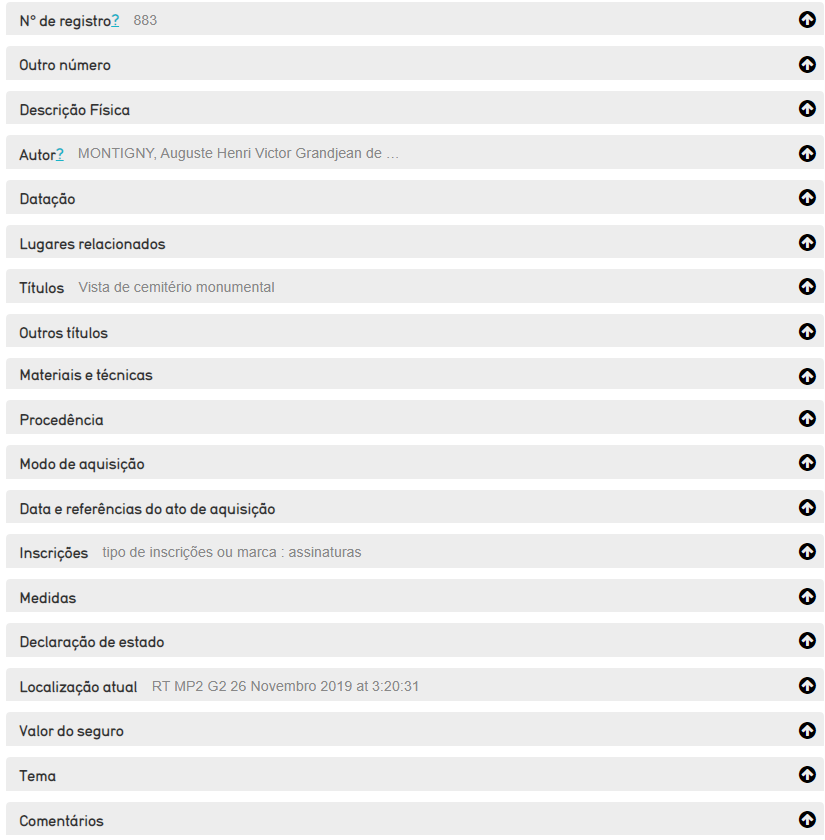
\includegraphics[width=\linewidth]{fichaId-01}
%	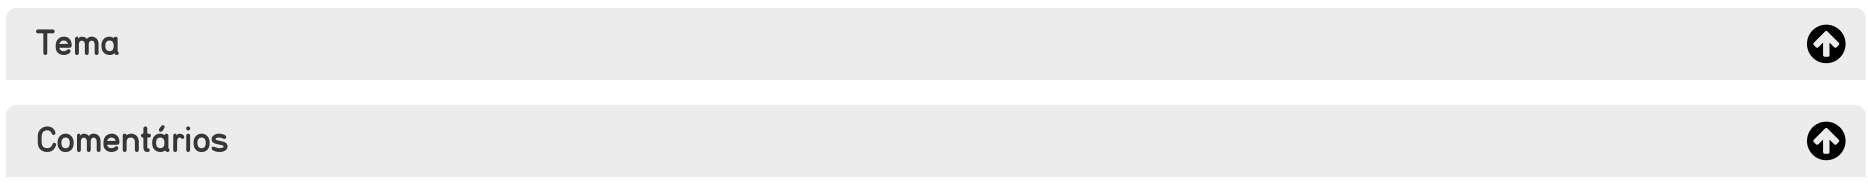
\includegraphics[width=\linewidth]{fichaId-02}
\end{flushleft}
%\begin{flushleft}
%	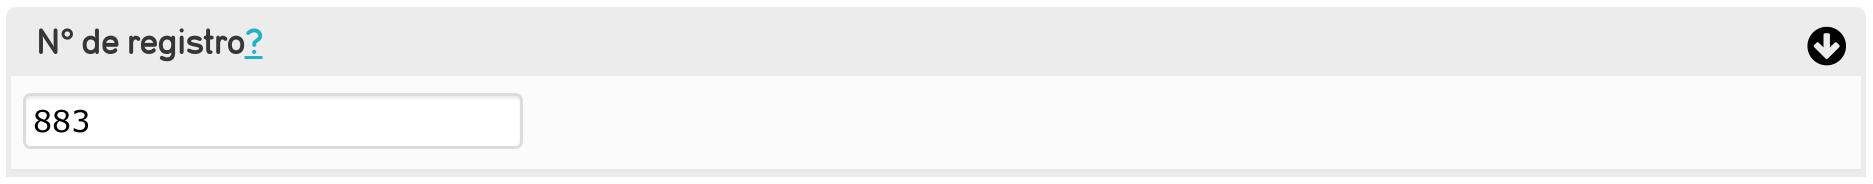
\includegraphics[width=\linewidth]{elemento-01}
%	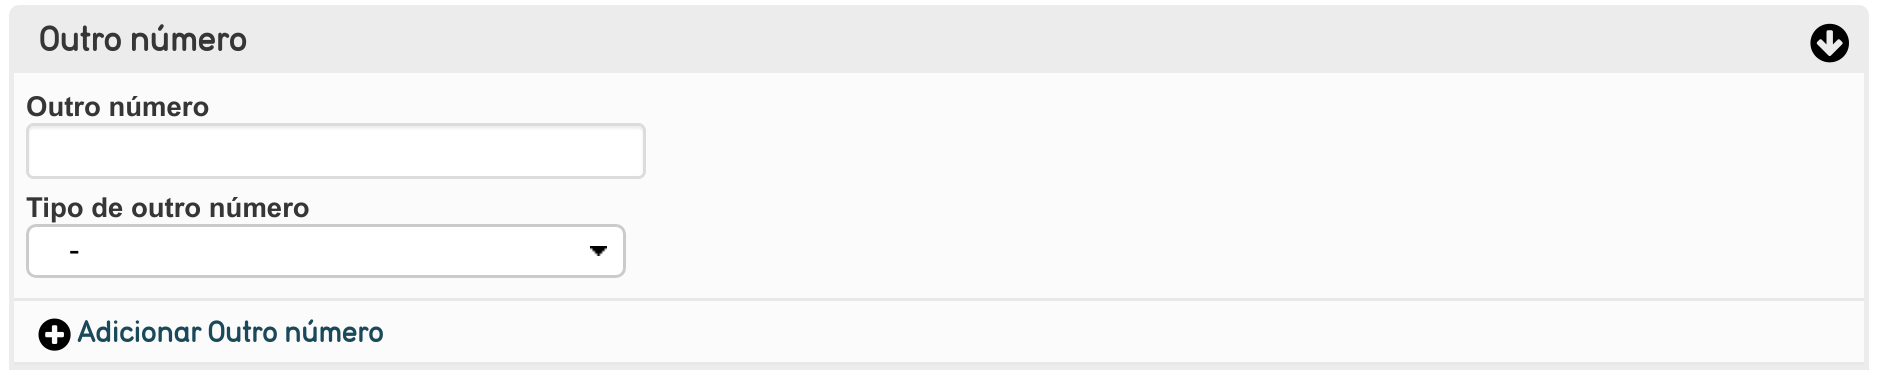
\includegraphics[width=\linewidth]{elemento-02}
%	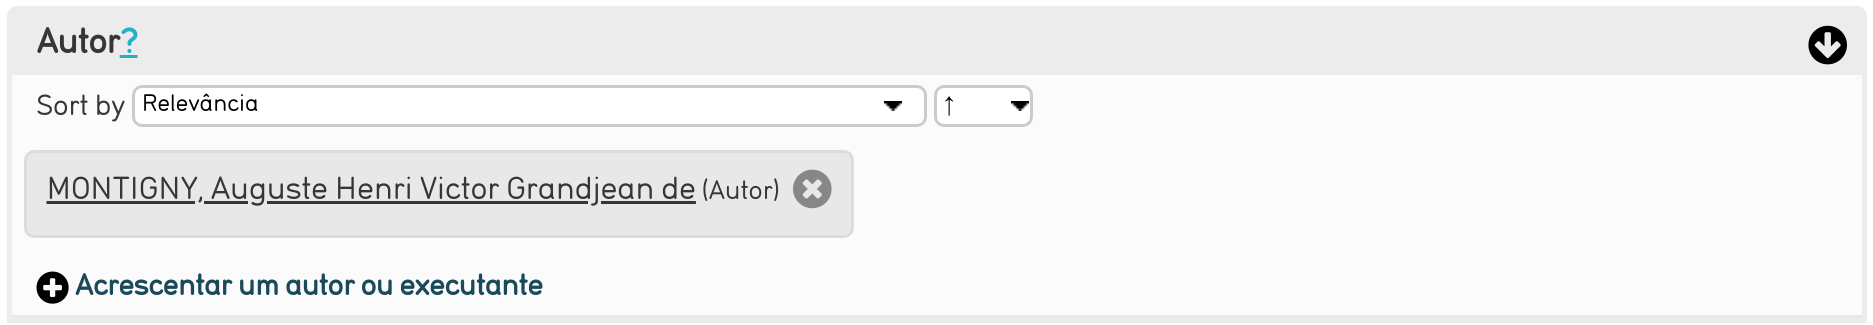
\includegraphics[width=\linewidth]{autor-01}
%	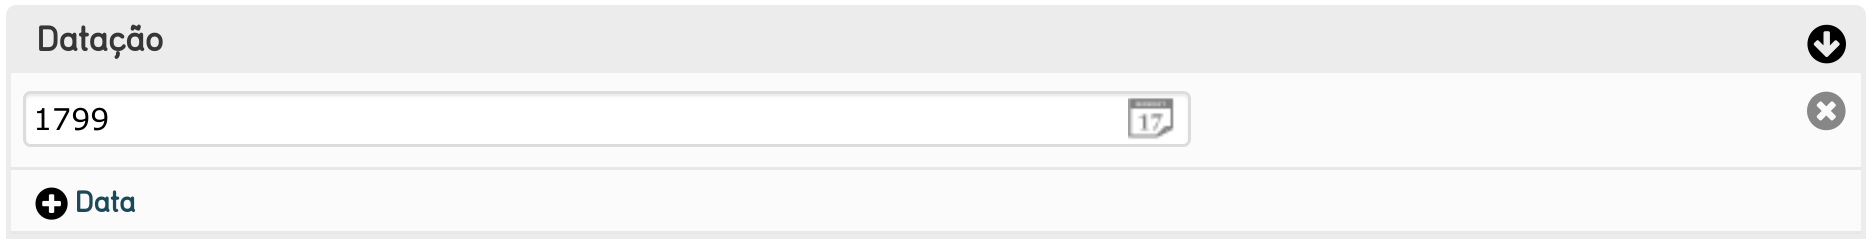
\includegraphics[width=\linewidth]{elemento-03}
%	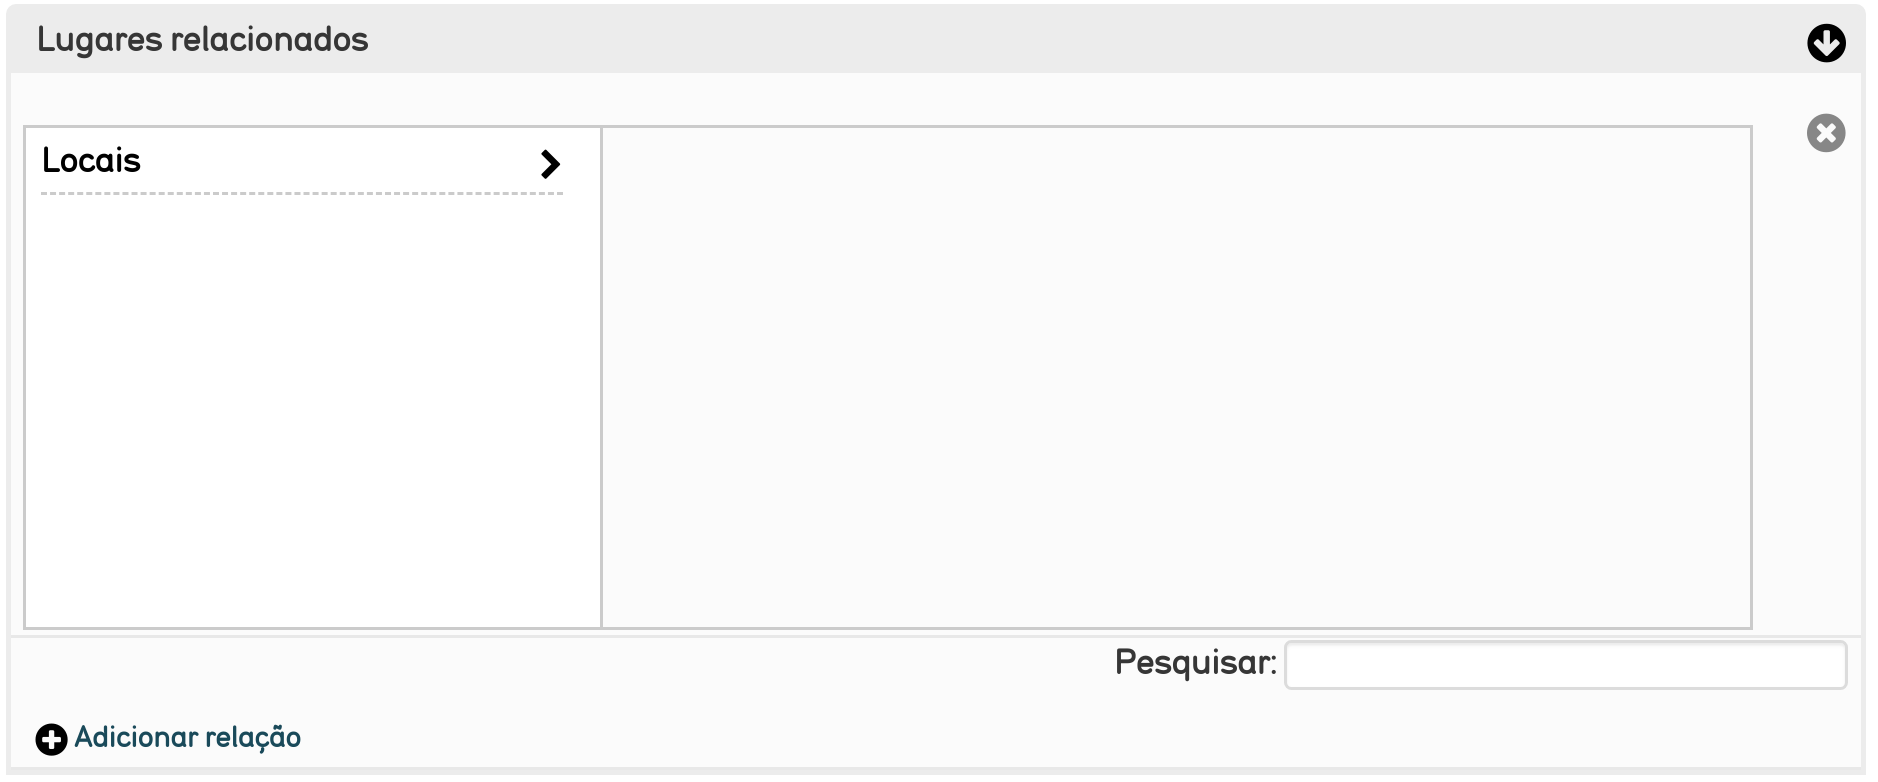
\includegraphics[width=\linewidth]{elemento-04}
%	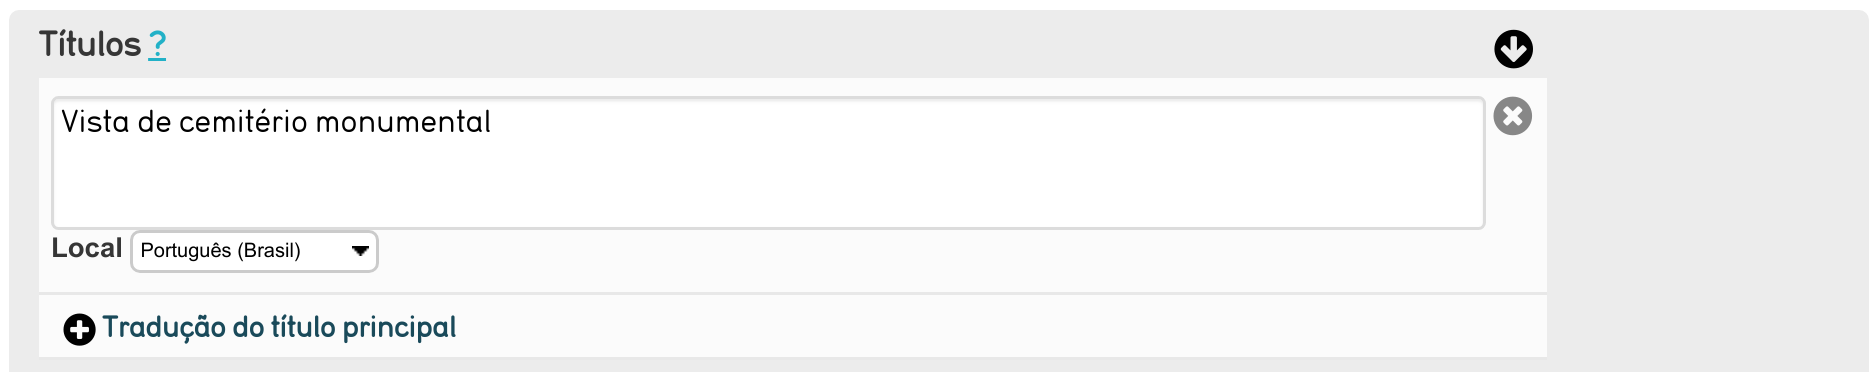
\includegraphics[width=\linewidth]{elemento-05}
%	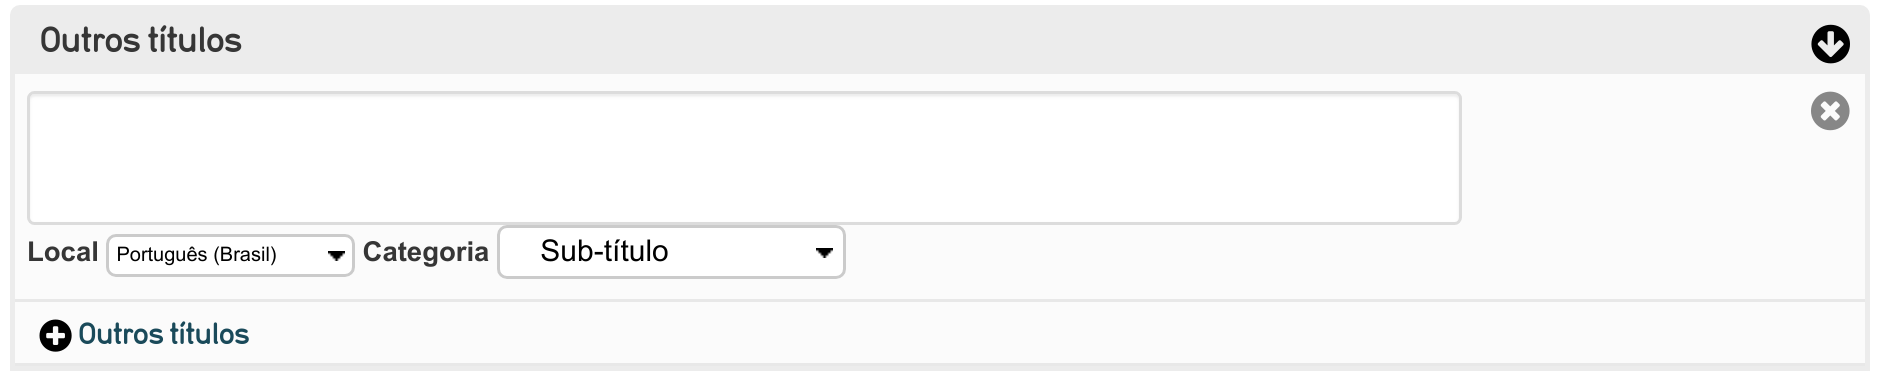
\includegraphics[width=\linewidth]{elemento-06}
%	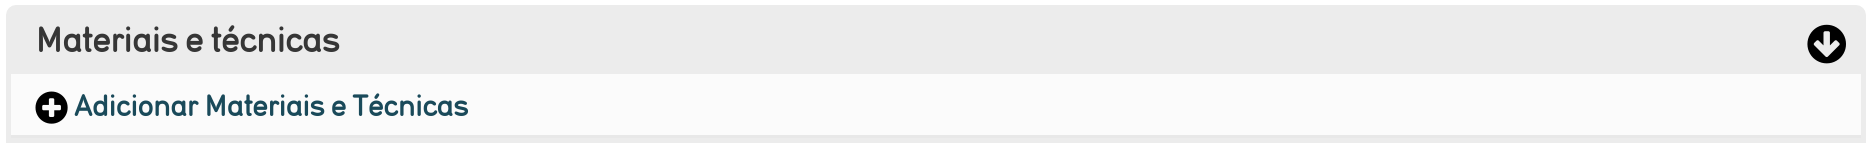
\includegraphics[width=\linewidth]{elemento-07}
%	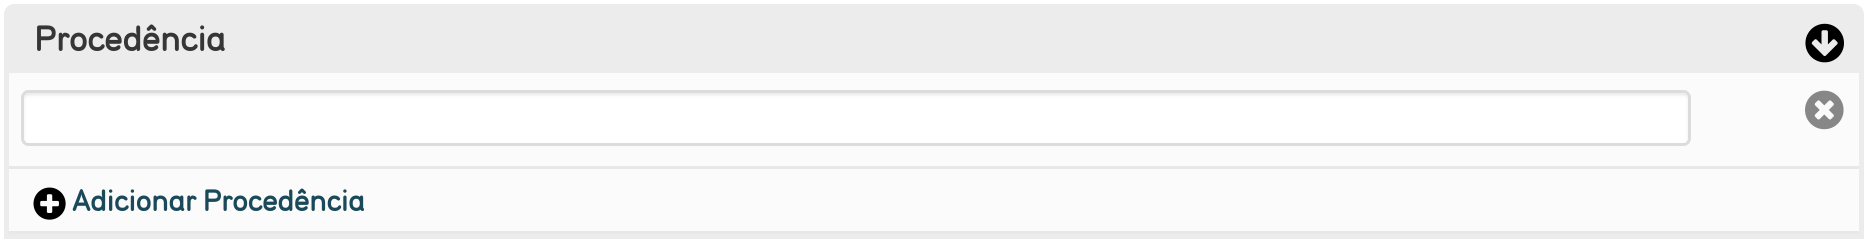
\includegraphics[width=\linewidth]{elemento-08}
%	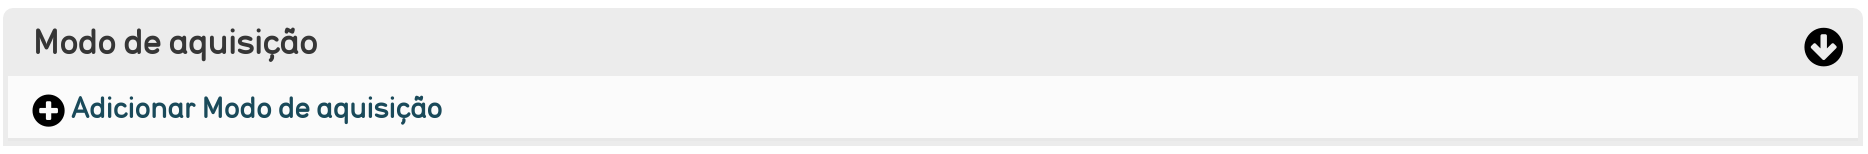
\includegraphics[width=\linewidth]{elemento-09}
%	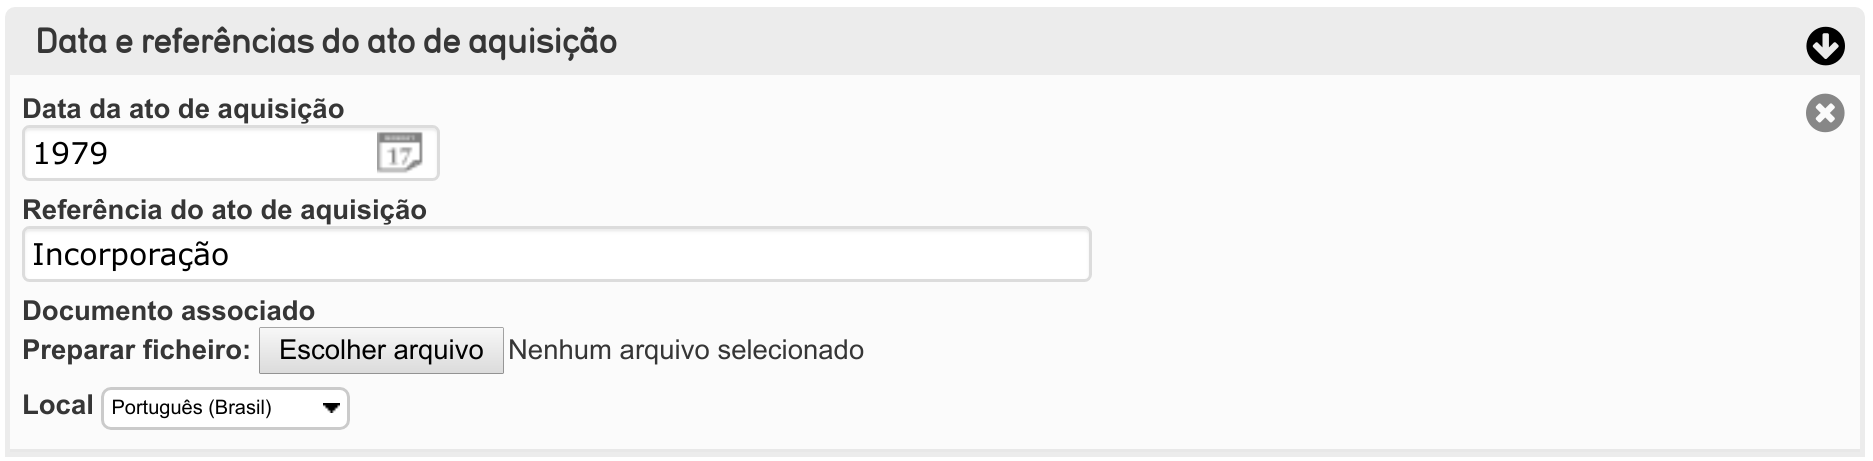
\includegraphics[width=\linewidth]{elemento-10}
%	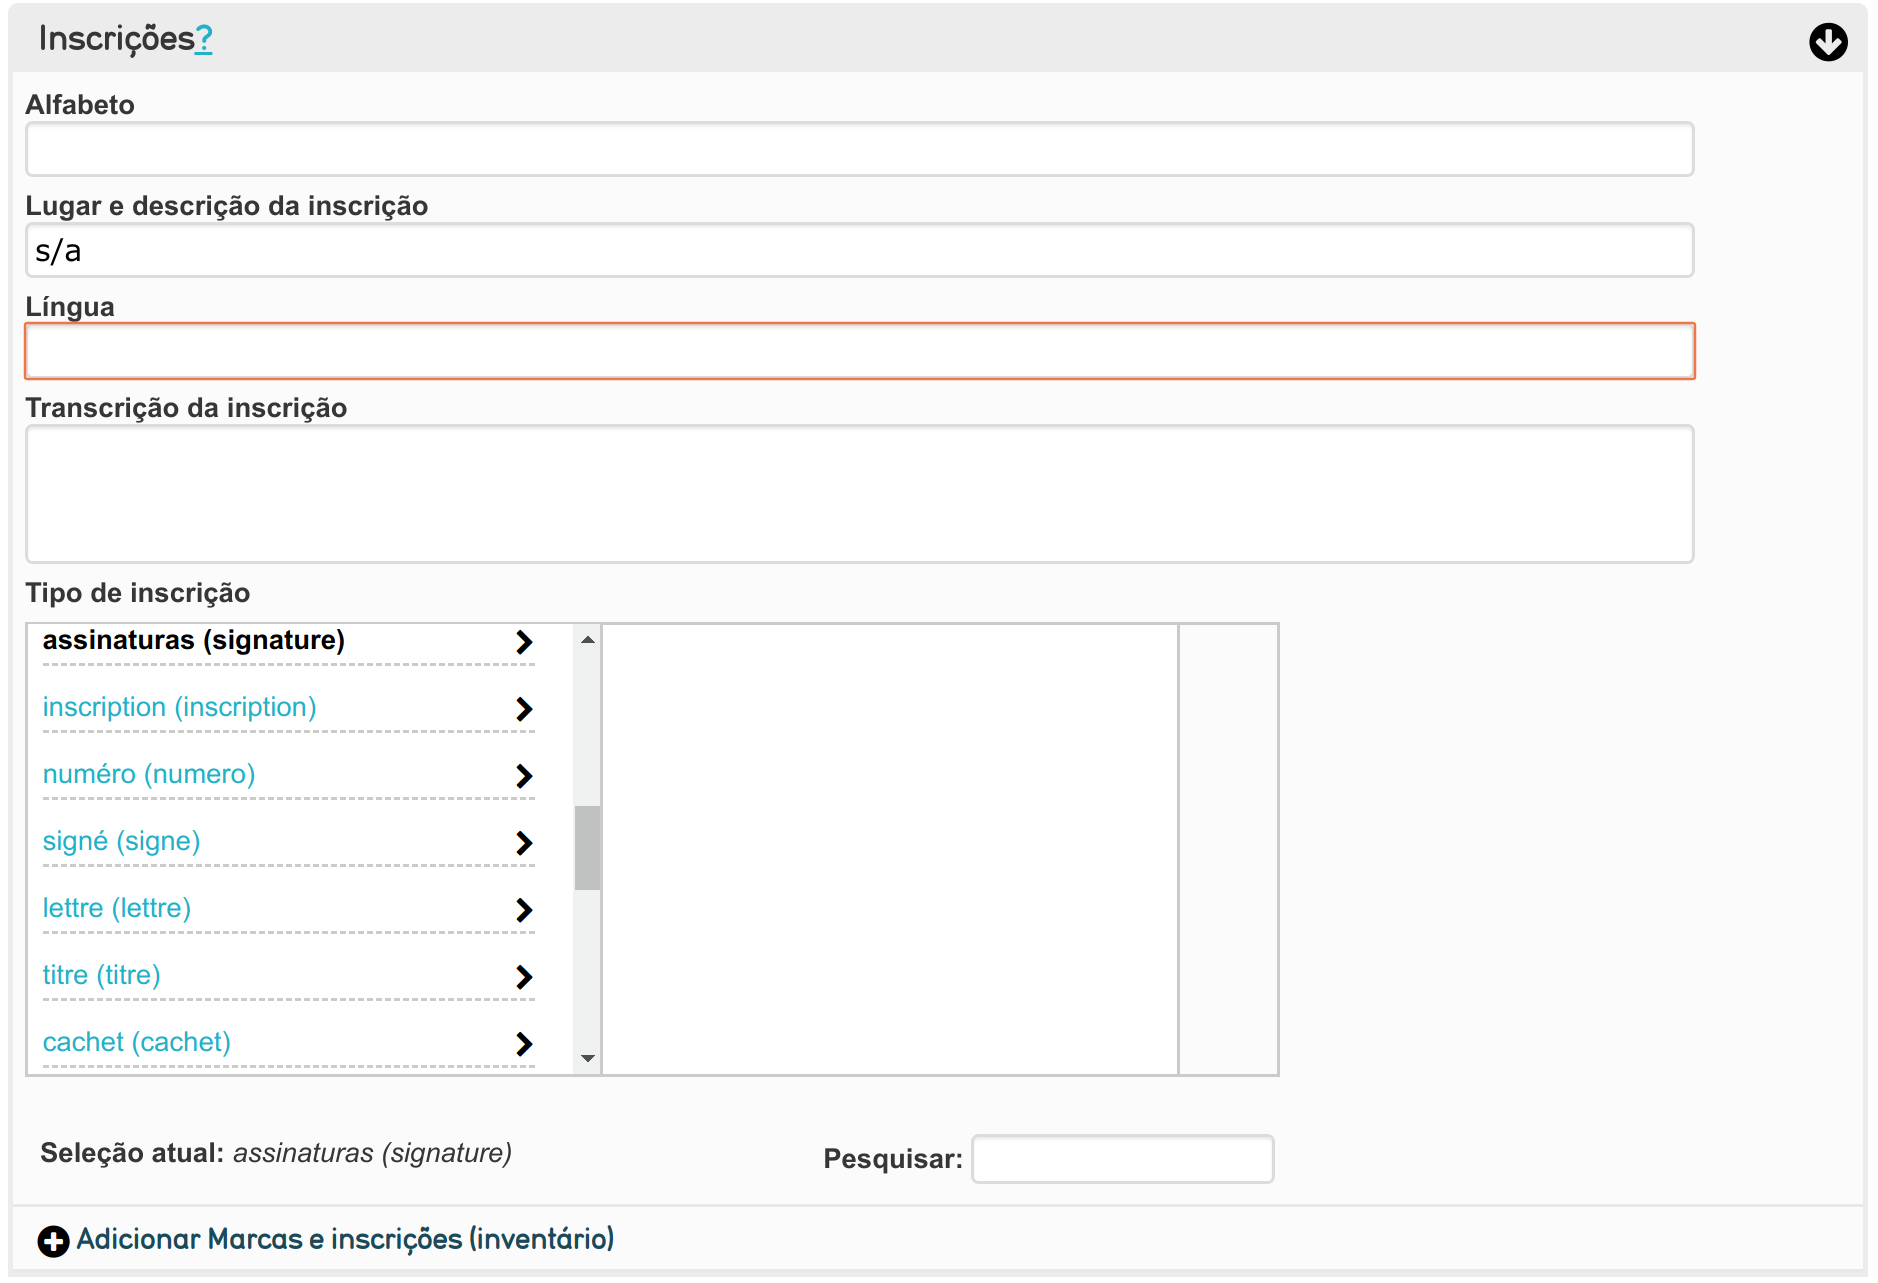
\includegraphics[width=\linewidth]{elemento-11}
%	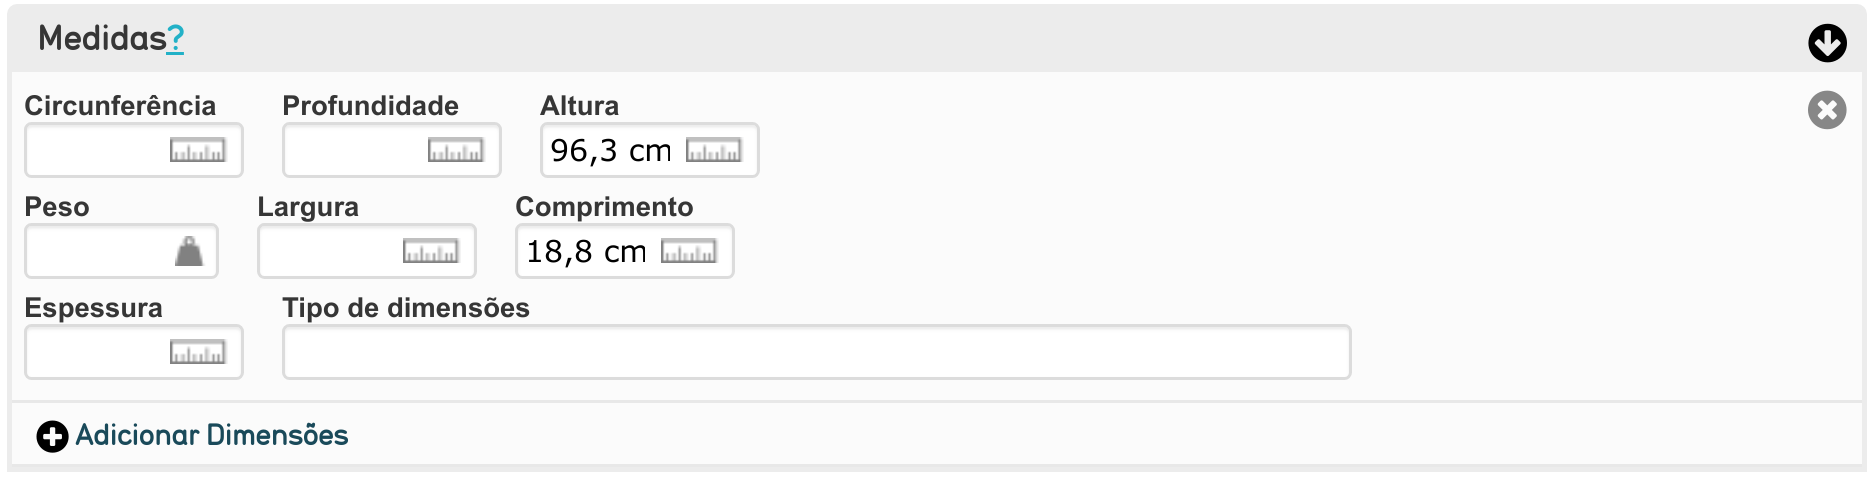
\includegraphics[width=\linewidth]{elemento-12}
%	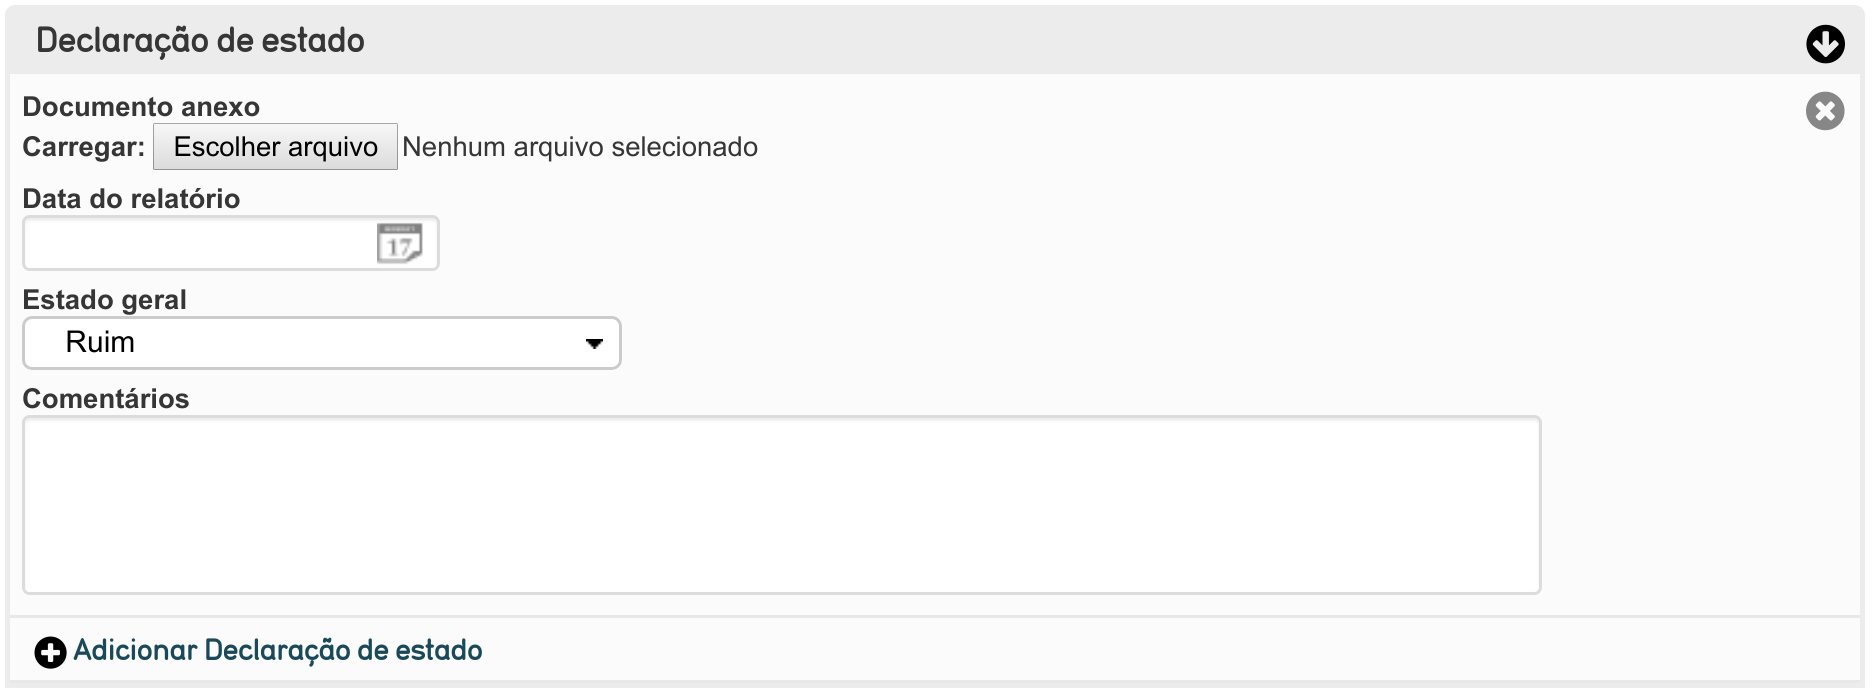
\includegraphics[width=\linewidth]{elemento-13}
%	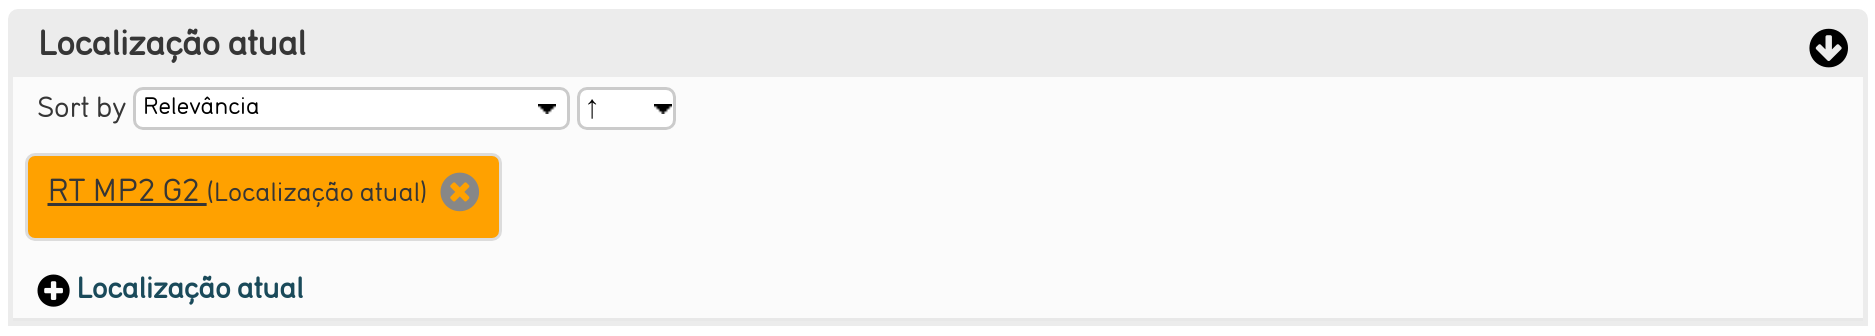
\includegraphics[width=\linewidth]{elemento-14}
%	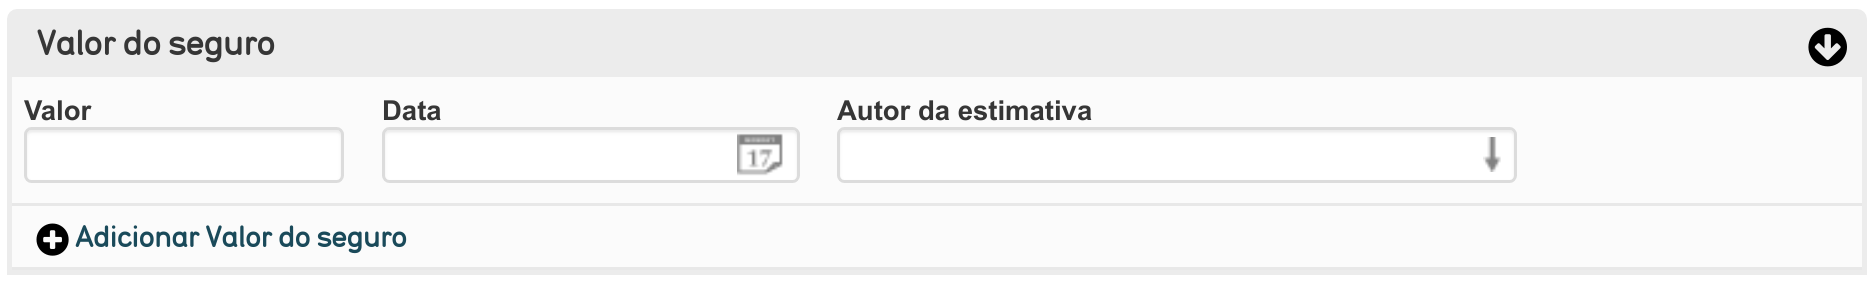
\includegraphics[width=\linewidth]{elemento-15}
%	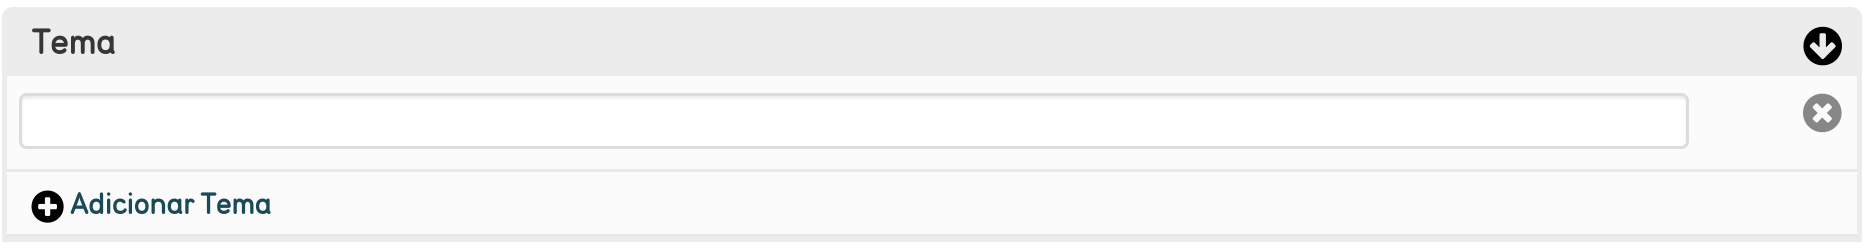
\includegraphics[width=\linewidth]{elemento-16}
%	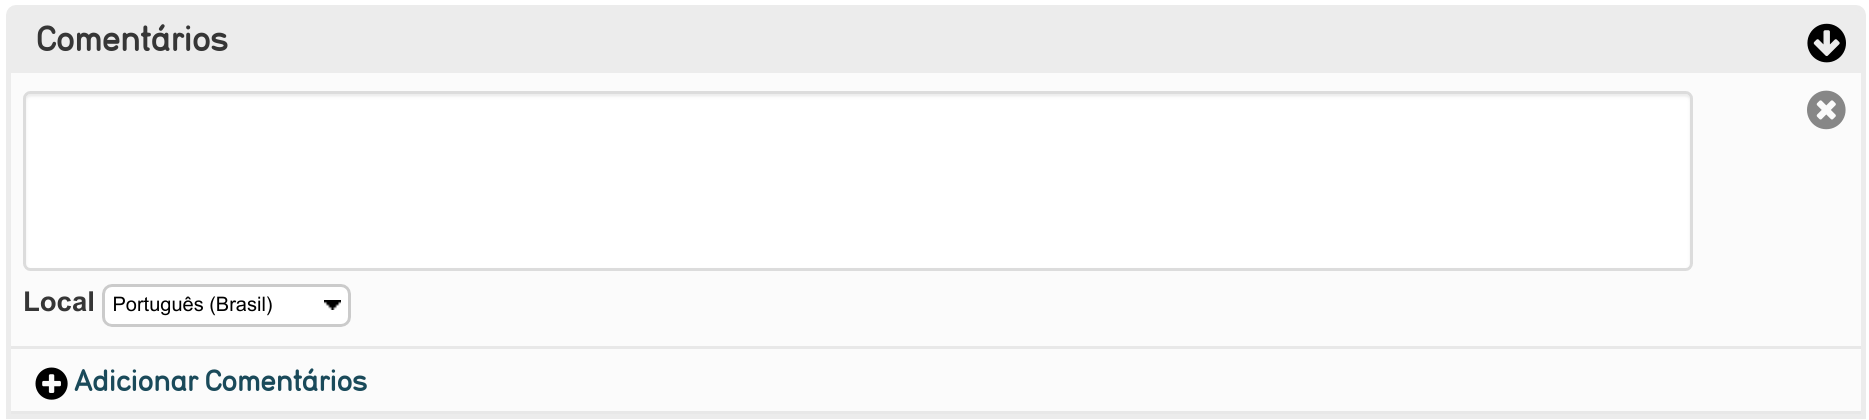
\includegraphics[width=\linewidth]{elemento-17}
%	
%\end{flushleft}
\subsection{Nº de registro}
\begin{flushleft}
	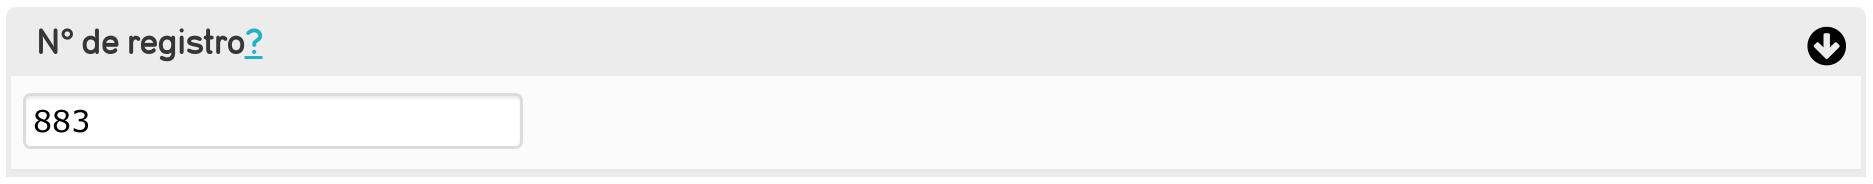
\includegraphics[width=\linewidth]{elemento-01}
\end{flushleft}
É o \textbf{número de registro de tombamento}. A numeração respeitou parcialmente o sistema numérico do Livro de Tombo encontrado, seguindo portanto, a sequência natural do número de ordem deste livro, cuja última peça fora registrada sob o número 2140. A primeira peça sem registro a ser inventariada recebeu, consequentemente, o número 2141.

Para tornar o sistema de numeração mais objetivo, optou-se por manter somente o número de ordem, abandonando o modelo tripartido do livro de tombo original, ou seja, omitindo-se os dígitos referentes ao ano de entrada da peça e a sua categoria. 

Para as peças compostas de diversas panes adotou-se o uso do complemento alfabético:

\begin{itemize}
	\item registro 1463 A - Classe Objetos Pessoais, Subclasse Objetos de adorno, Relógio - e 
	\item 1463 B - Classe Objetos pessoais, Subclasse Objetos de adorno, Estojo.
\end{itemize}

\subsection{Outro número}
\begin{flushleft}
	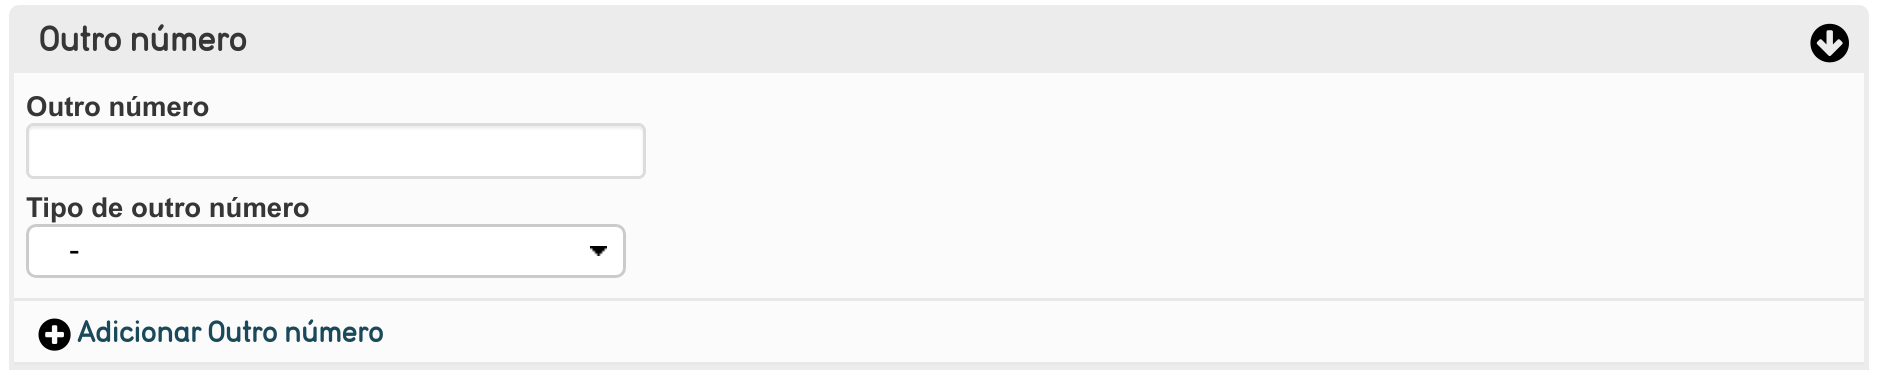
\includegraphics[width=\linewidth]{elemento-02}
\end{flushleft}
Alguma outra referência para o objeto. O tipo de número também pode ser especificado:
\begin{itemize}
	\item Antigo número do inventário
	\item Ficha do museu
	\item Número antigo
	\item Número de classificação
	\item Número de inventário na coleção do depositante
	\item Número dentro da coleção do proprietário
	\item Número de verificação
	\item Número no Registro da UFRJ
\end{itemize}
\begin{flushleft}
	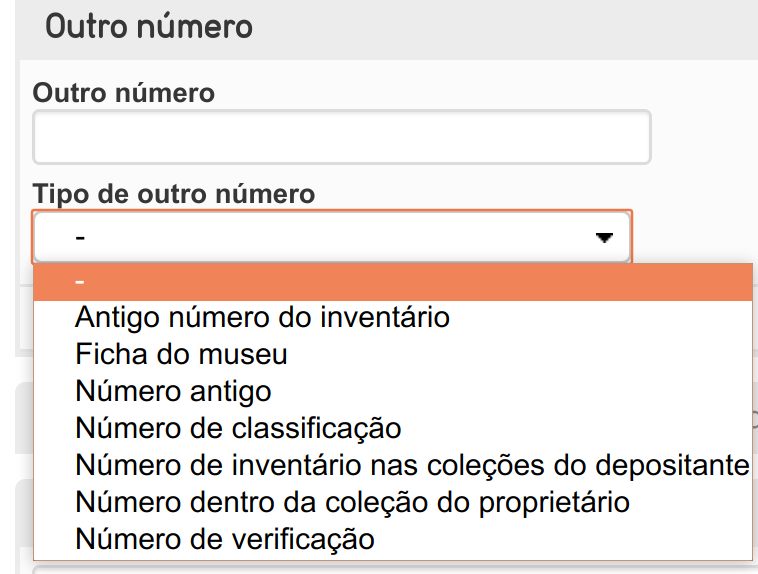
\includegraphics[width=0.5\linewidth]{tipoOutroNumero}
\end{flushleft}

\subsection{Descrição Física}

\begin{flushleft}
	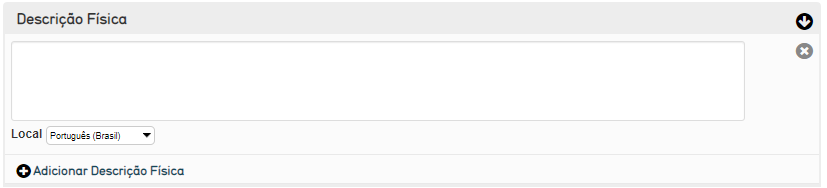
\includegraphics[width=\linewidth]{DescricFisica}
\end{flushleft}

Campo destinado à escrita livre sobre a descrição física do objeto.

\subsection{Autor}
\begin{flushleft}
	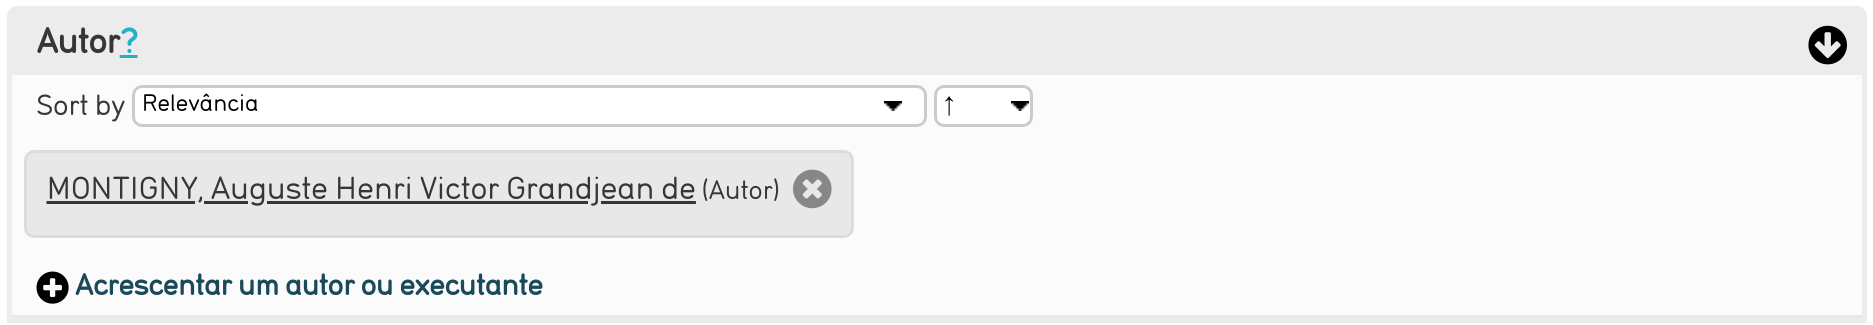
\includegraphics[width=\linewidth]{autor-01}
\end{flushleft}
Campo destinado ao registro de pessoa física ou jurídica que concebeu material e/ou intelectualmente a obra. Podem ser acrescentados outros autores.

\subsection{Datação}
\begin{flushleft}
	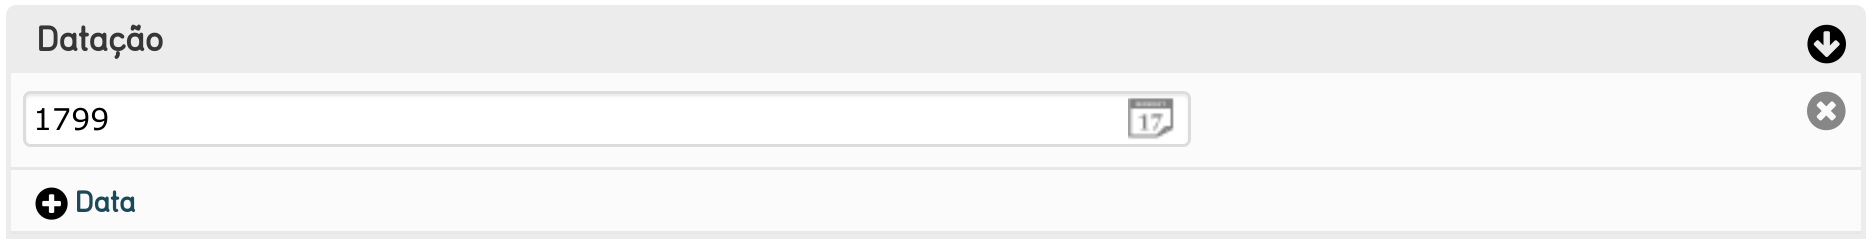
\includegraphics[width=\linewidth]{elemento-03}
\end{flushleft}

\subsection{Lugares relacionados}
\begin{flushleft}
	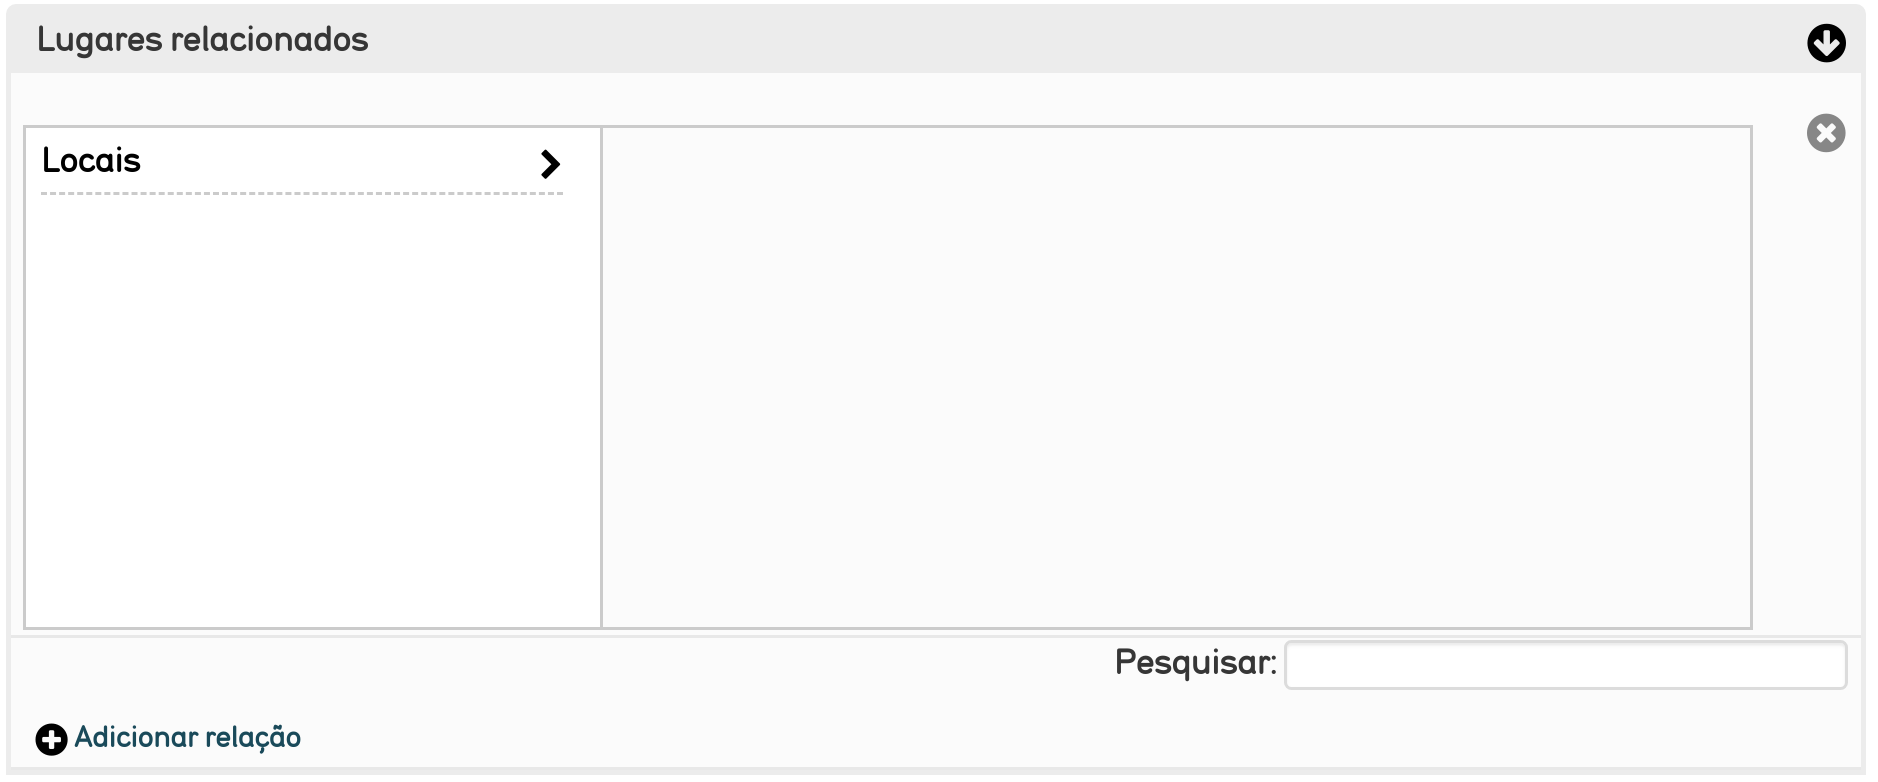
\includegraphics[width=\linewidth]{elemento-04}
\end{flushleft}

Além do lugar relacionado também se deve escolher a relação do lugar com a obra por meio do menu disponível.

\begin{flushleft}
	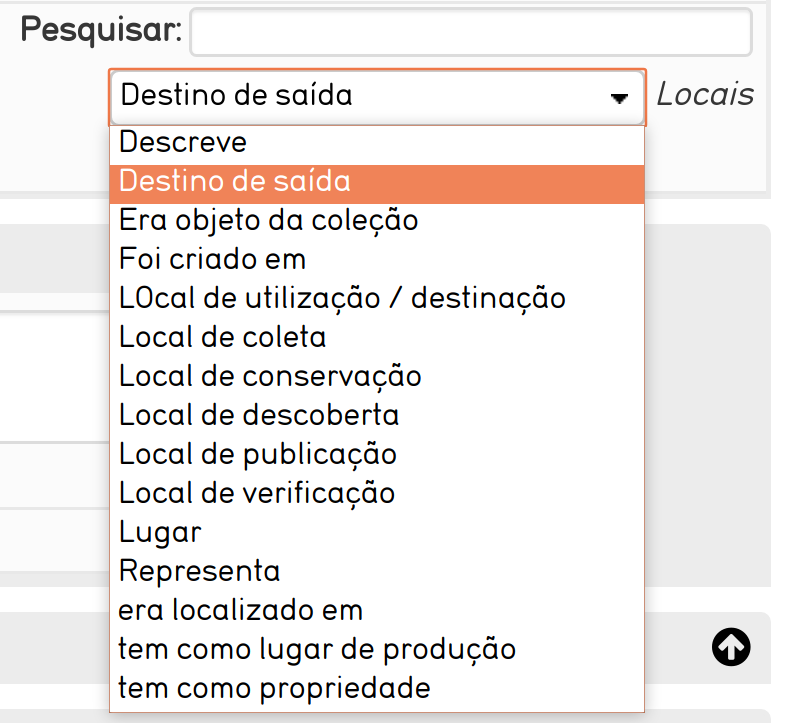
\includegraphics[width=0.5\linewidth]{descreveLugar}
\end{flushleft}

\subsection{Títulos}
\begin{flushleft}
	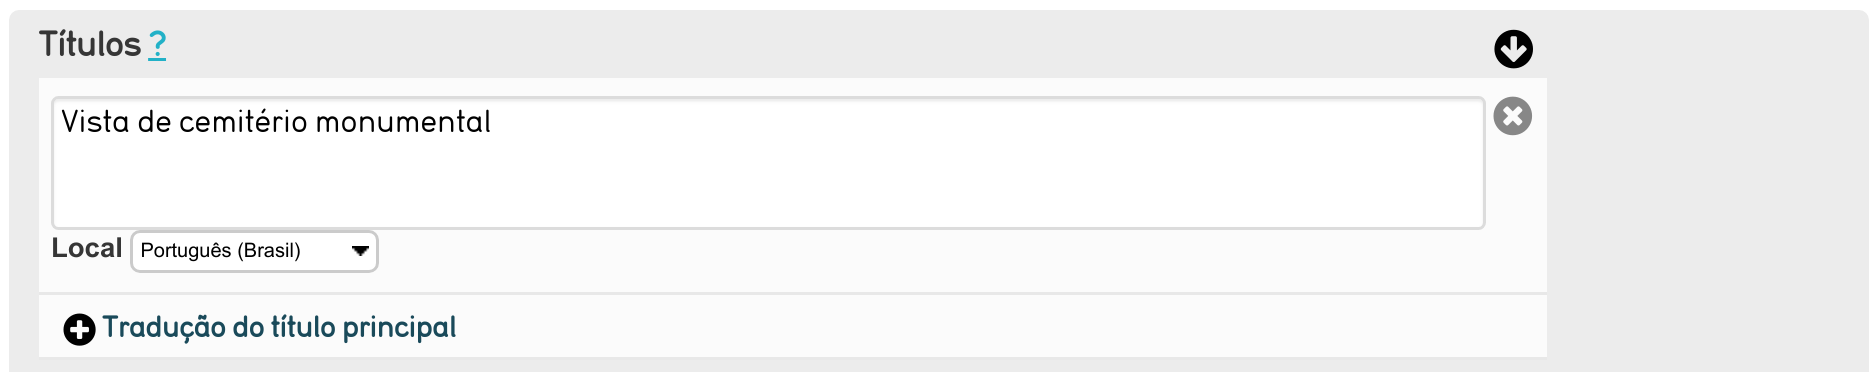
\includegraphics[width=\linewidth]{elemento-05}
\end{flushleft}
Também é possível fornecer uma tradução em outras línguas do título da obra.

\subsection{Outros títulos}
\begin{flushleft}
	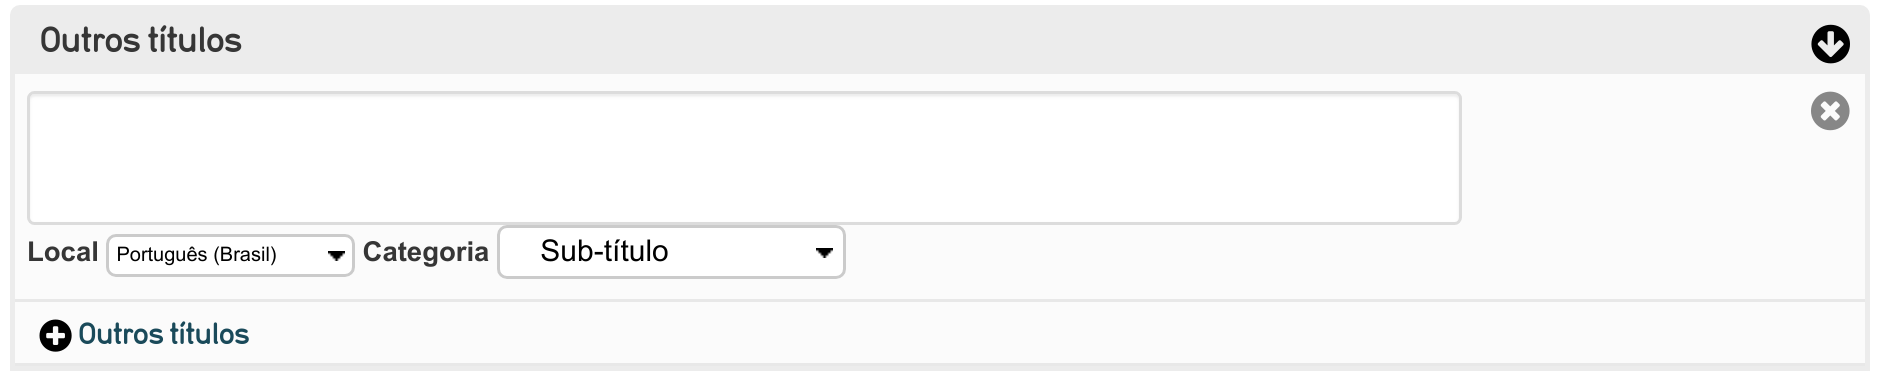
\includegraphics[width=\linewidth]{elemento-06}
\end{flushleft}

\subsection{Materiais e técnicas}
\begin{flushleft}
	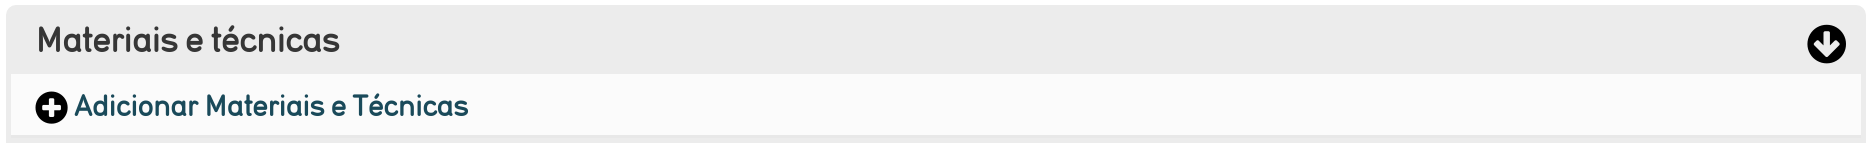
\includegraphics[width=\linewidth]{elemento-07}
\end{flushleft}

\subsection{Procedência}
\begin{flushleft}
	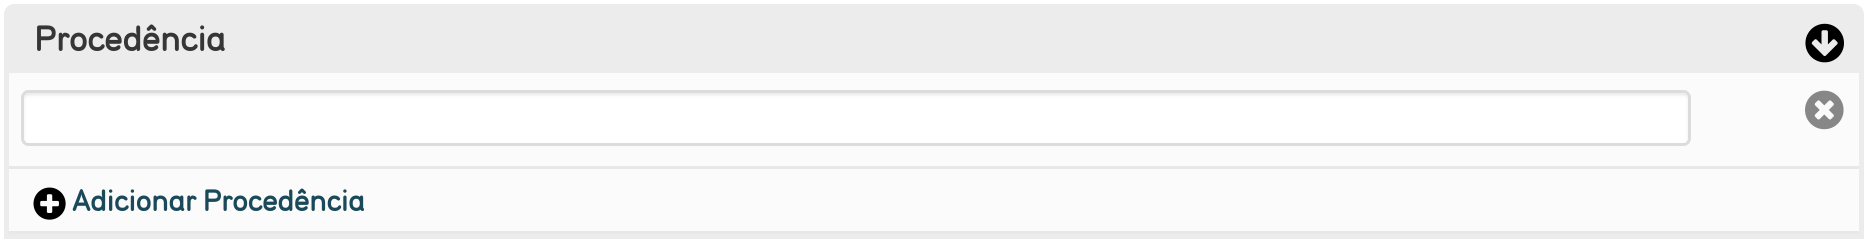
\includegraphics[width=\linewidth]{elemento-08}
\end{flushleft}

\subsection{Modo de aquisição}
\begin{flushleft}
	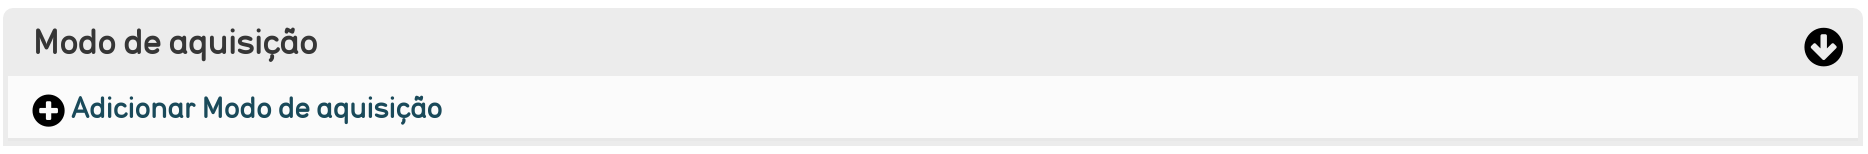
\includegraphics[width=\linewidth]{elemento-09}
\end{flushleft}

\subsection{Data e referências so ato de aquisição}
\begin{flushleft}
	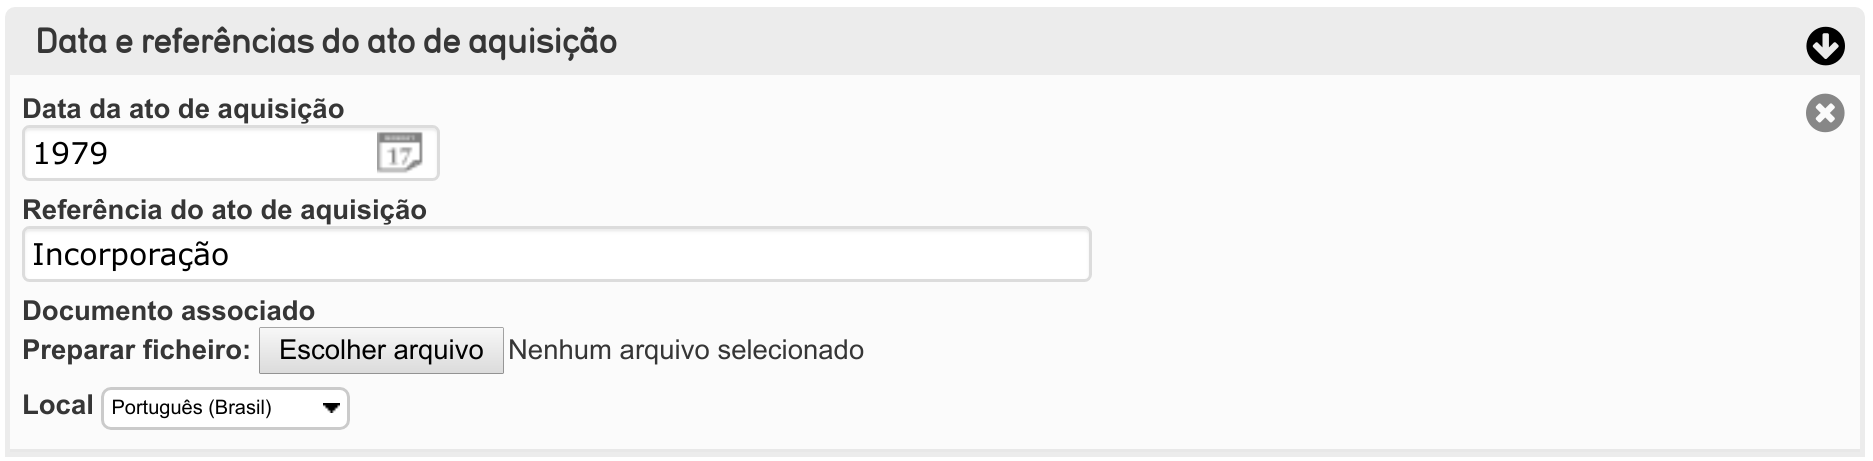
\includegraphics[width=\linewidth]{elemento-10}
\end{flushleft}

\subsection{Inscrições}
\begin{flushleft}
	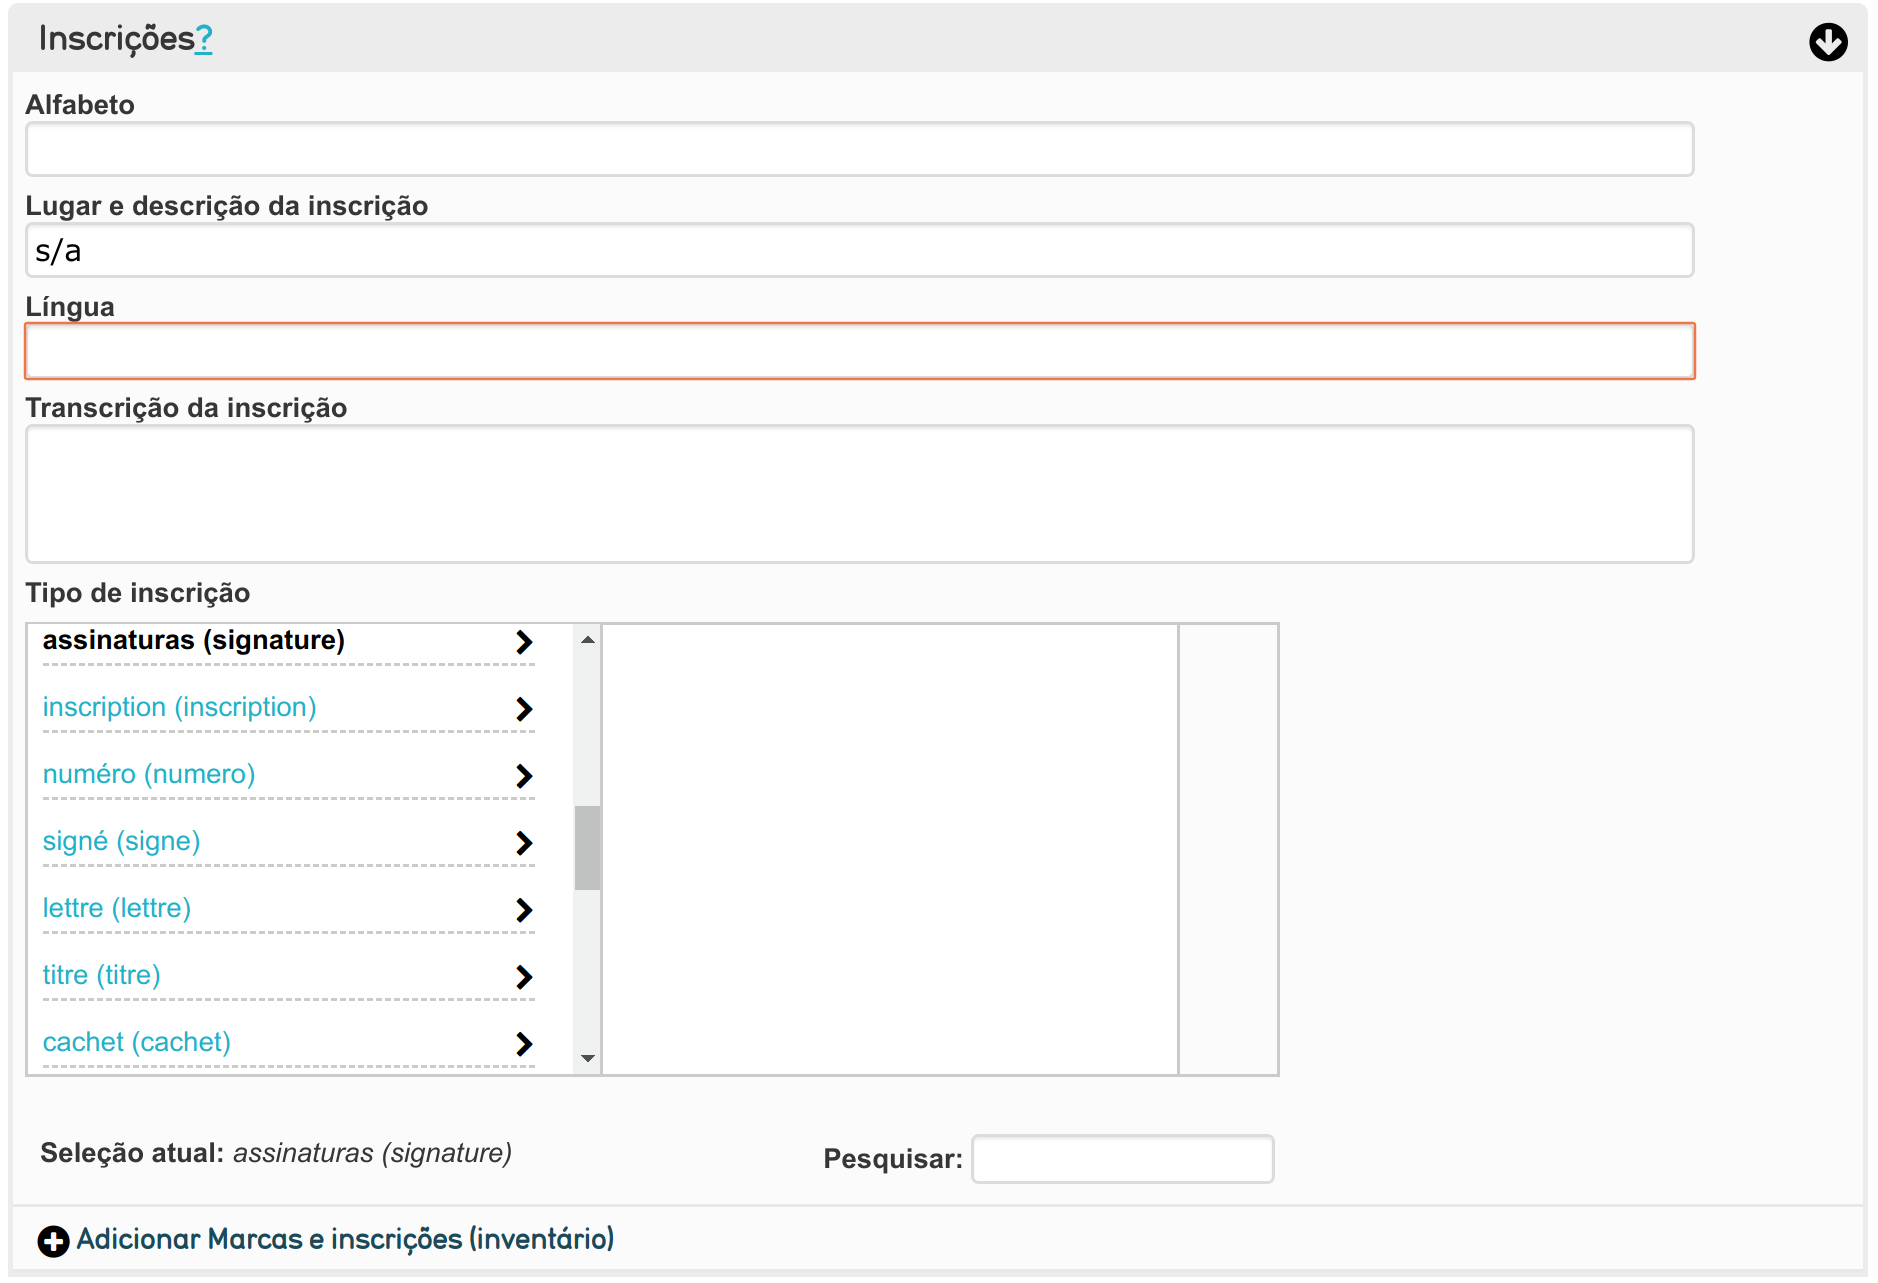
\includegraphics[width=\linewidth]{elemento-11}
\end{flushleft}

\subsection{Medidas}
\begin{flushleft}
	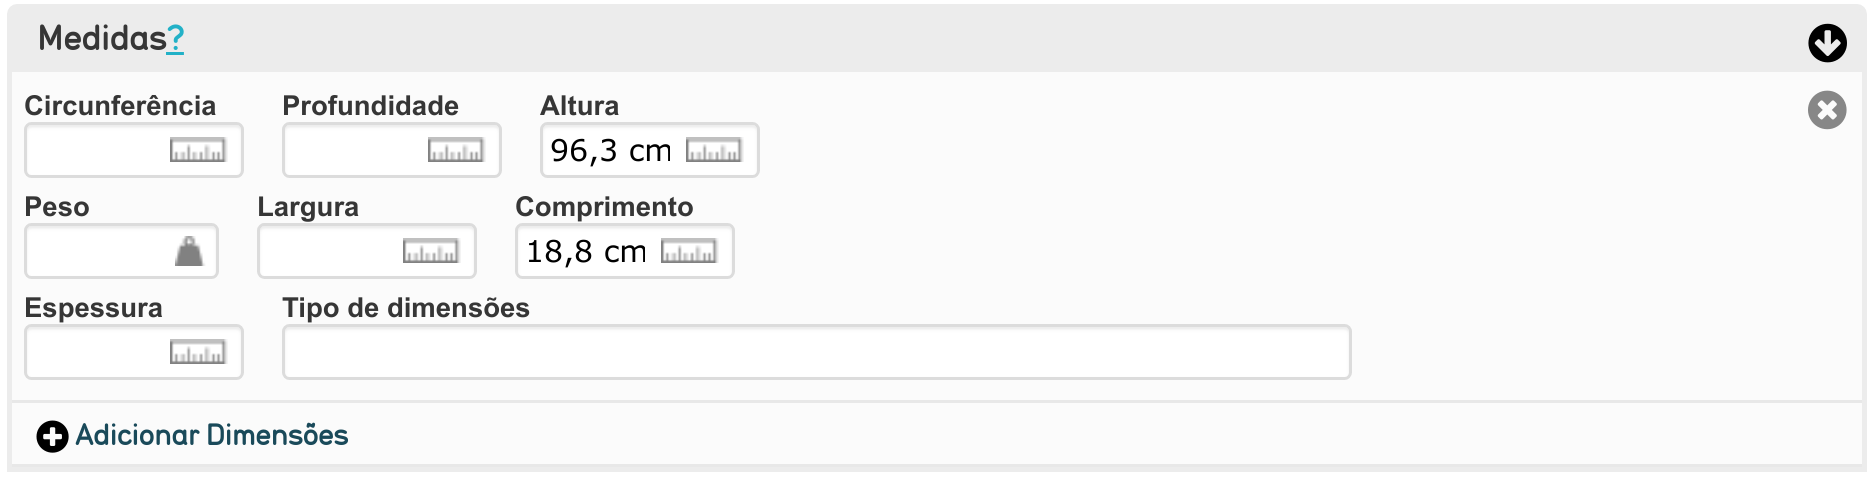
\includegraphics[width=\linewidth]{elemento-12}
\end{flushleft}

\subsection{Declaração de estado}
\begin{flushleft}
	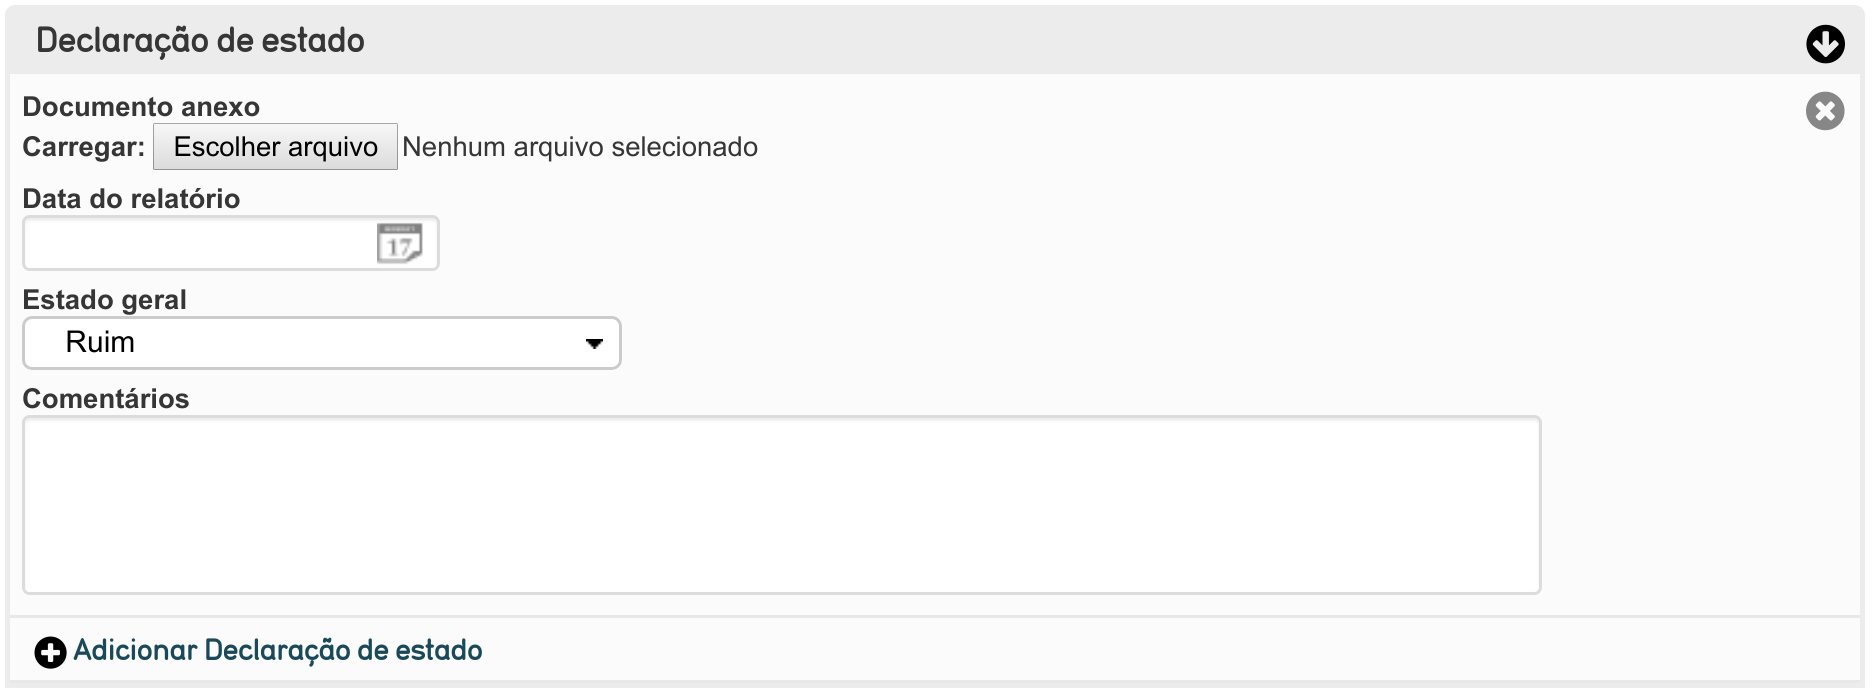
\includegraphics[width=\linewidth]{elemento-13}
\end{flushleft}

\subsection{Localização atual}
\begin{flushleft}
	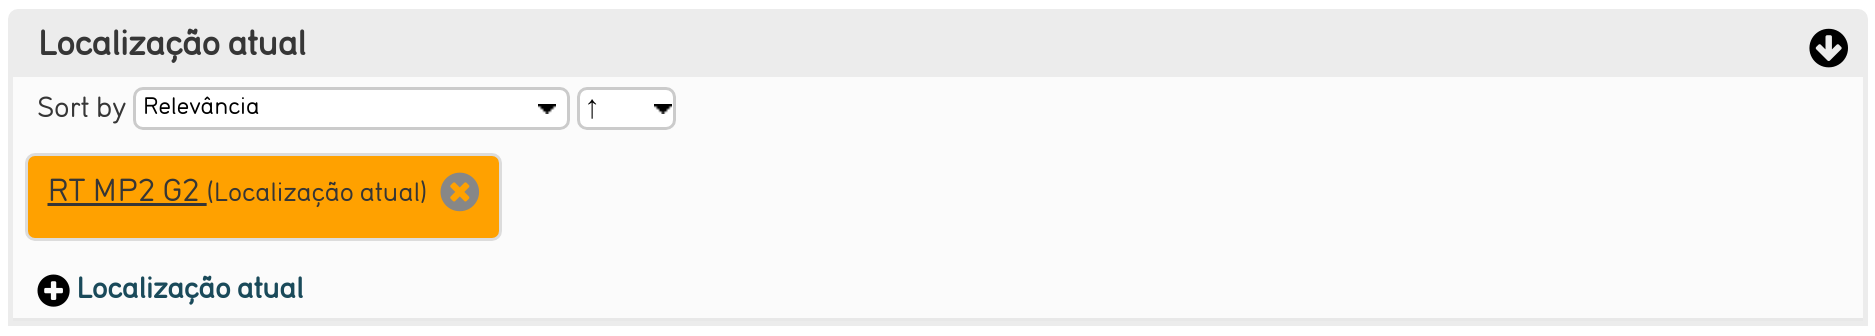
\includegraphics[width=\linewidth]{elemento-14}
\end{flushleft}

\subsection{Valor do seguro}
\begin{flushleft}
	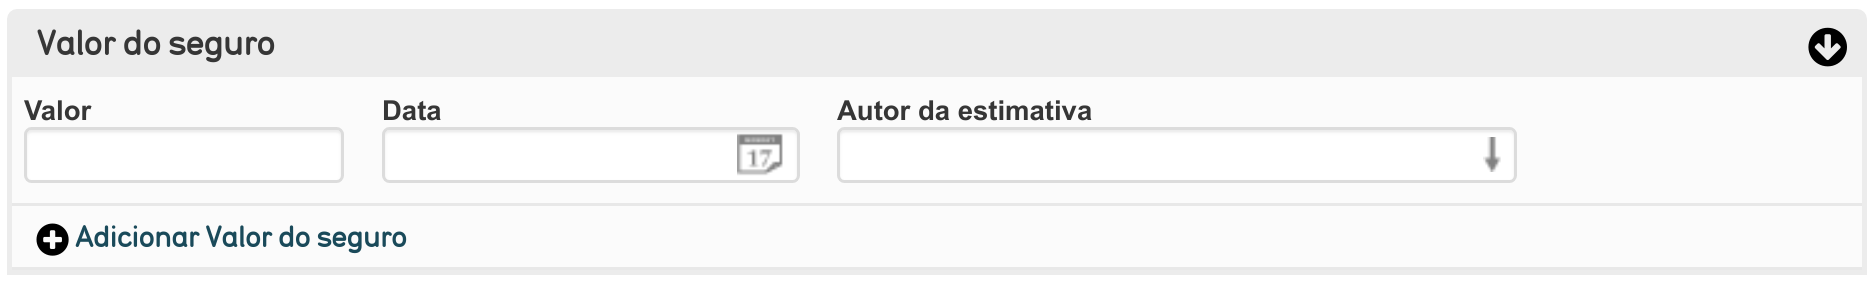
\includegraphics[width=\linewidth]{elemento-15}
\end{flushleft}

\subsection{Tema}
\begin{flushleft}
	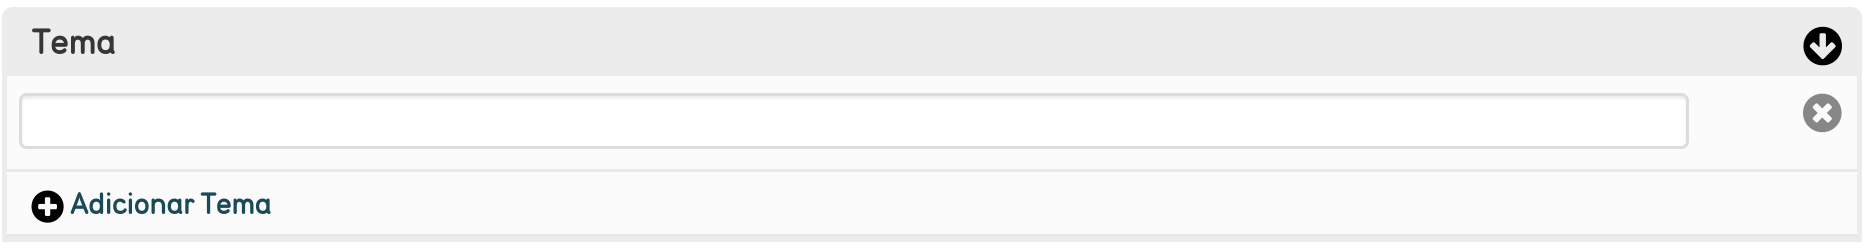
\includegraphics[width=\linewidth]{elemento-16}
\end{flushleft}

\subsection{Comentários}
\begin{flushleft}
	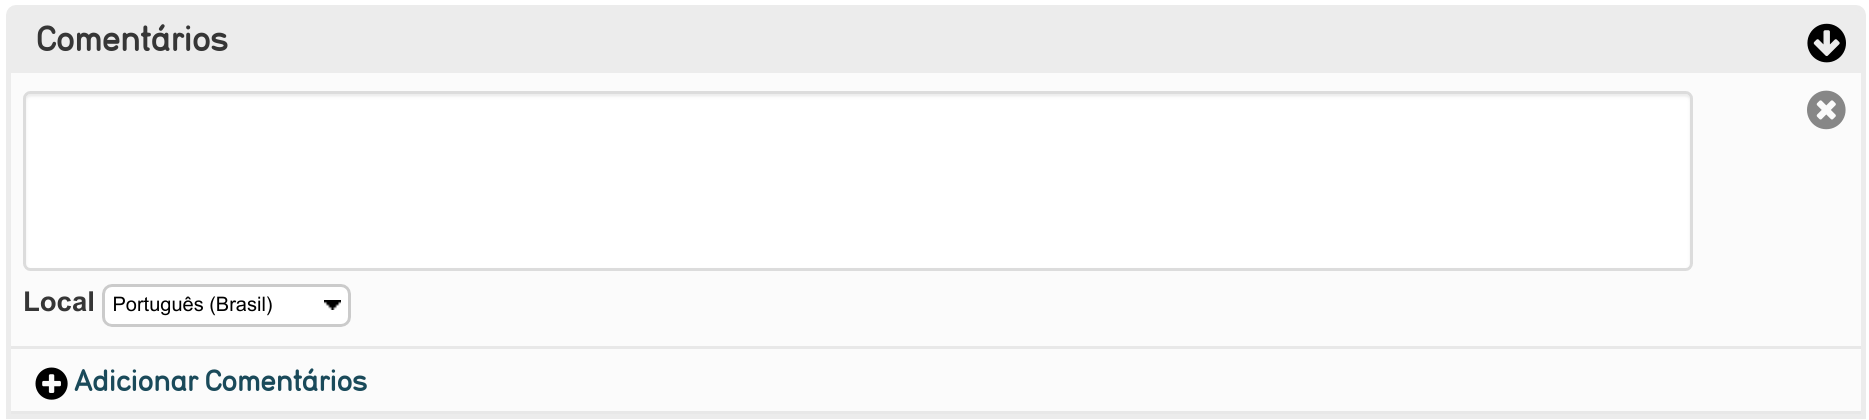
\includegraphics[width=\linewidth]{elemento-17}
\end{flushleft}

\section{Ficha Análise Histórica e Estilística}
\subsection{Visão Geral}
\begin{flushleft}
	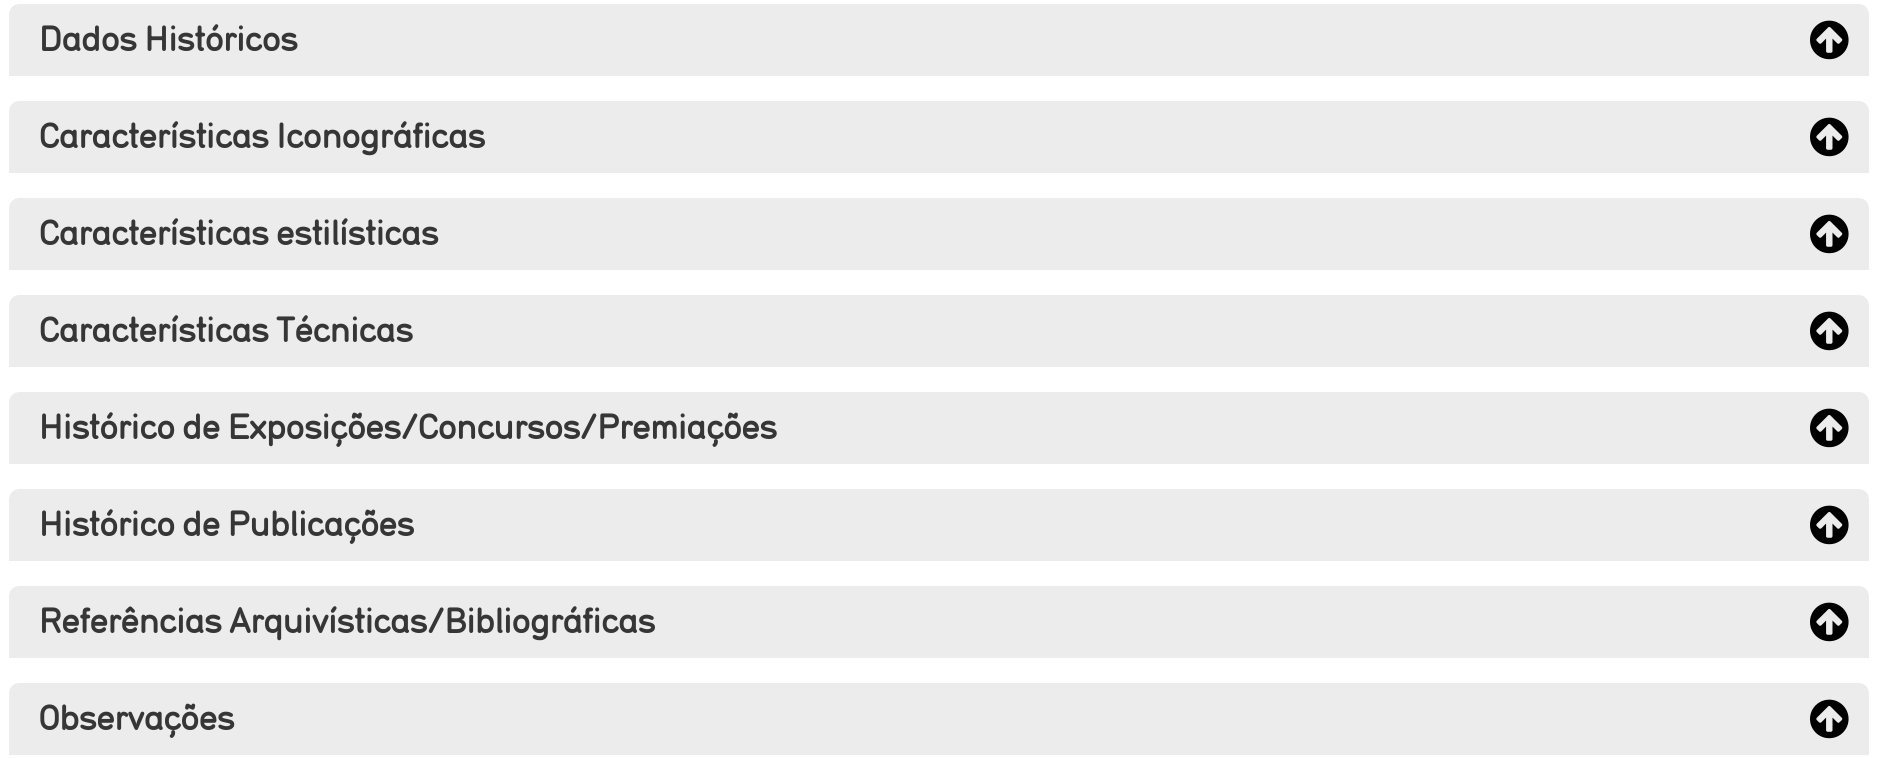
\includegraphics[width=\linewidth]{elementoFichaAnalise}
\end{flushleft}

\subsection{Dados Históricos}
\begin{flushleft}
	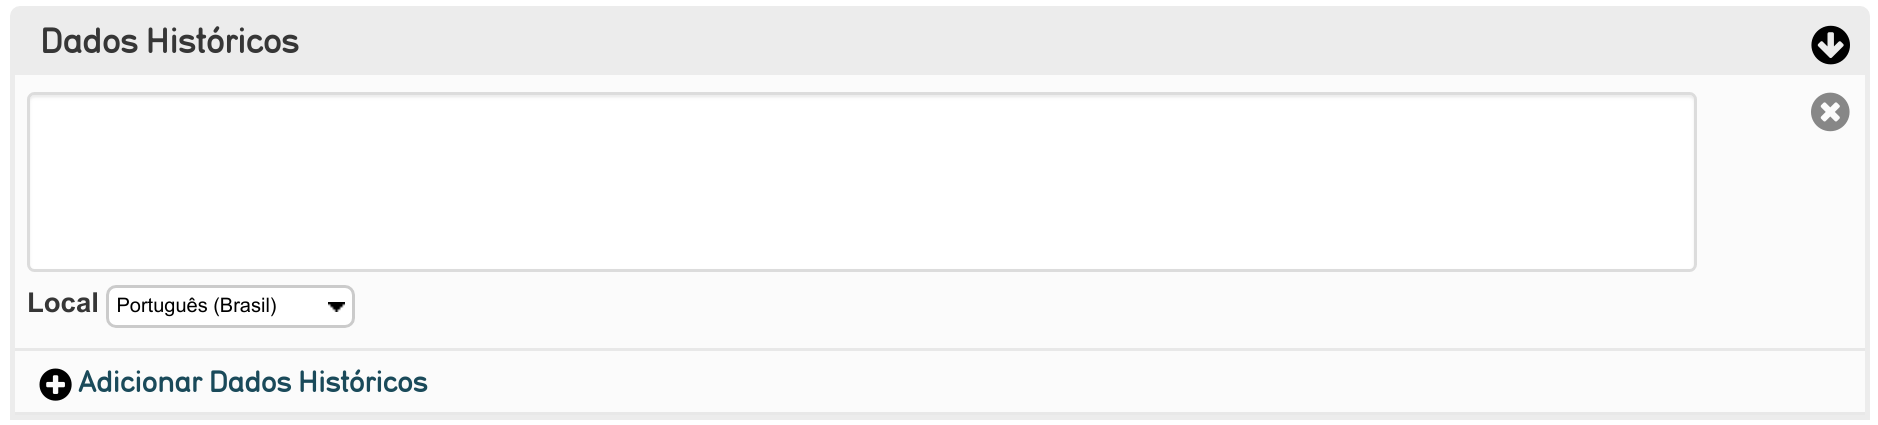
\includegraphics[width=\linewidth]{elemento-18}
\end{flushleft}

\subsection{Características Iconográficas}
\begin{flushleft}
	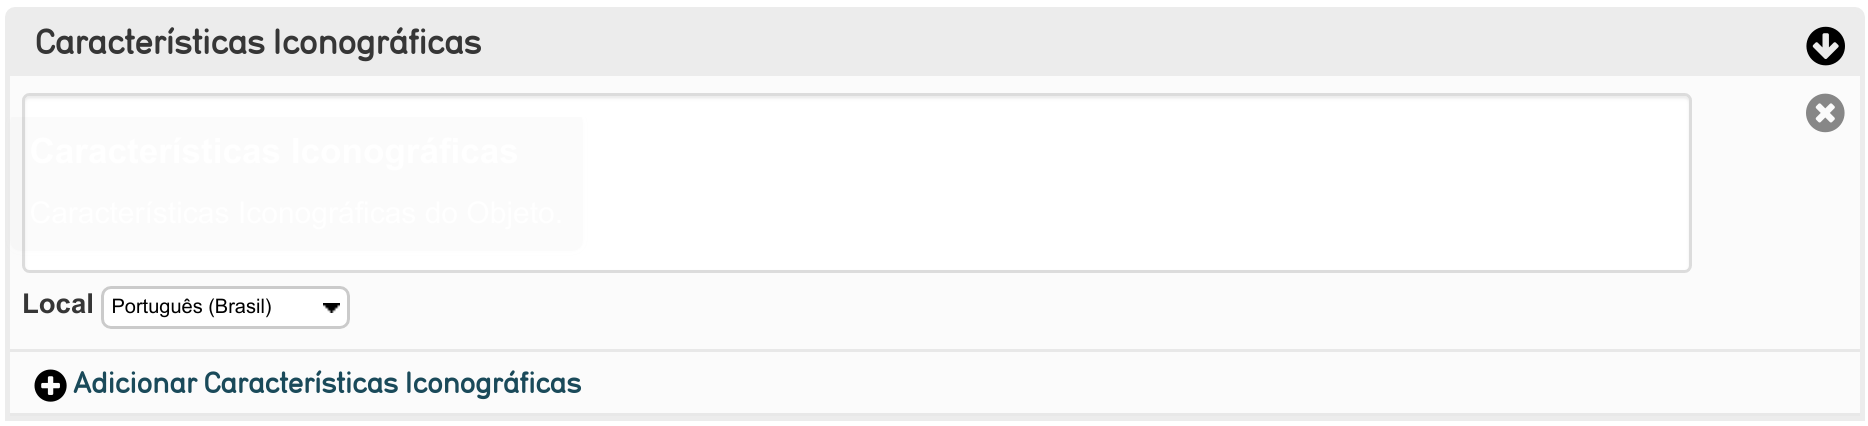
\includegraphics[width=\linewidth]{elemento-19}
\end{flushleft}

\subsection{Características Estilísticas}
\begin{flushleft}
	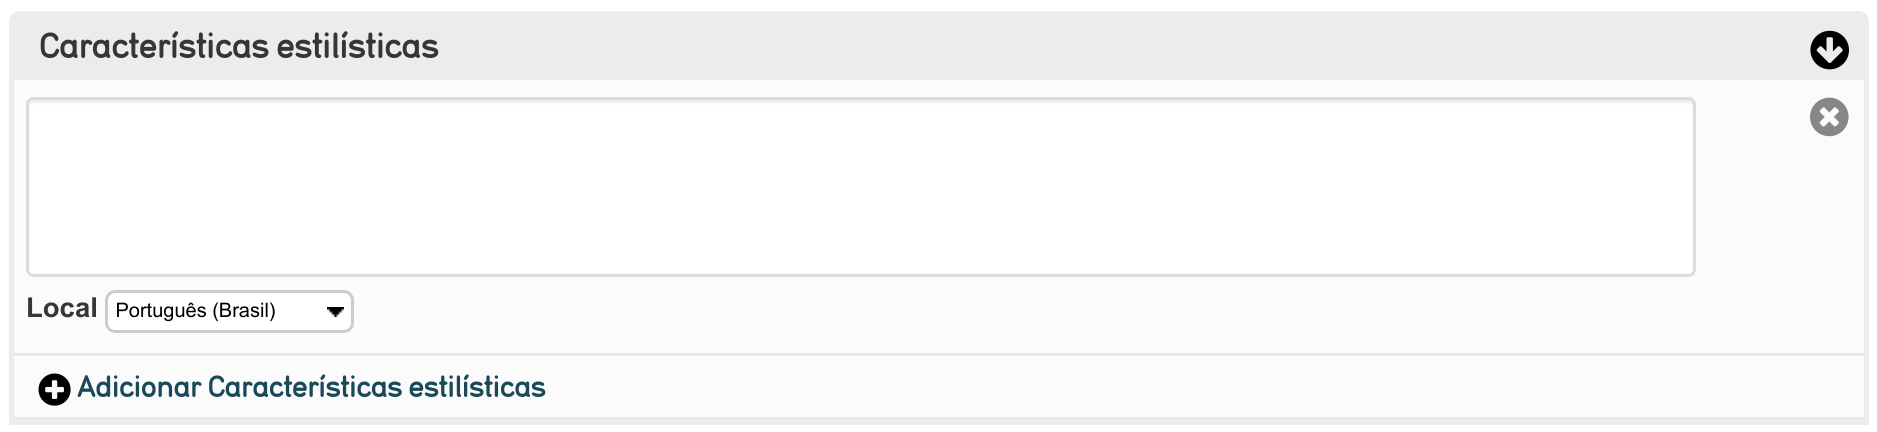
\includegraphics[width=\linewidth]{elemento-20}
\end{flushleft}

\subsection{Características Técnicas}
\begin{flushleft}
	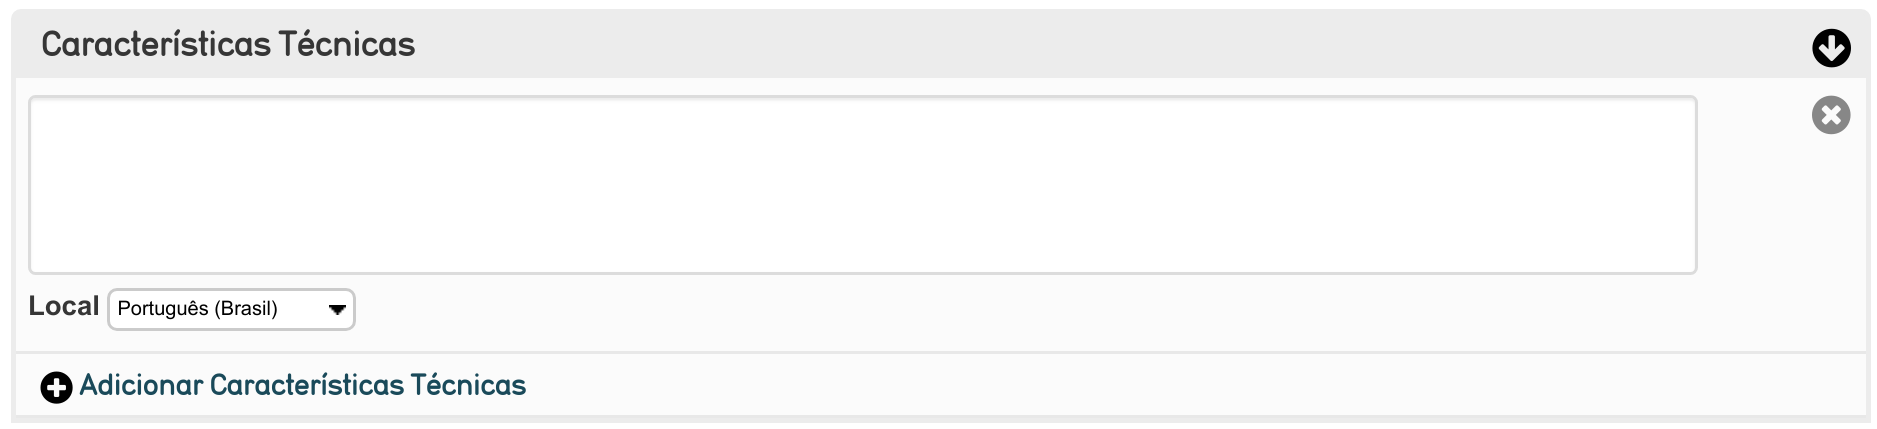
\includegraphics[width=\linewidth]{elemento-21}
\end{flushleft}

\subsection{Histórico de Exposições/Concursos/Premiações}
\begin{flushleft}
	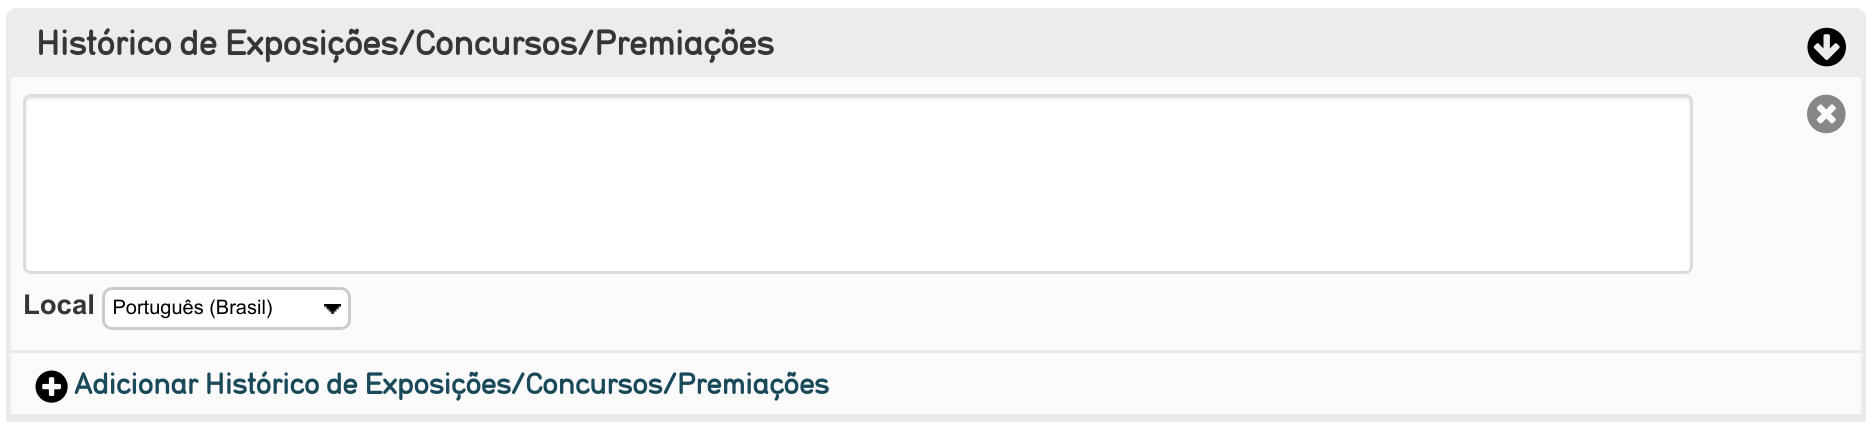
\includegraphics[width=\linewidth]{elemento-22}
\end{flushleft}

\subsection{Histórico de Publicações}
\begin{flushleft}
	\includegraphics[width=\linewidth]{elemento-23}
\end{flushleft}

\subsection{Referências Arquivísticas/Bibliográficas}
\begin{flushleft}
	\includegraphics[width=\linewidth]{elemento-24}
\end{flushleft}

\subsection{Observações}
\begin{flushleft}
	\includegraphics[width=\linewidth]{elemento-25}
\end{flushleft}

\includegraphics{resumo}

%===========================================================
%===========================================================
%XXXXXXXXXXXXXXXXXXXXXXXXXXXXXXXXXXXXXXXXXXXXXXXXXXXXXXXXXXX
% Anexos (opcionais)
%XXXXXXXXXXXXXXXXXXXXXXXXXXXXXXXXXXXXXXXXXXXXXXXXXXXXXXXXXXX
\annex % inicia os anexos
%XXXXXXXXXXXXXXXXXXXXXXXXXXXXXXXXXXXXXXXXXXXXXXXXXXXXXXXXXXX

%===========================================================
\postextualchapter{Primeiro anexo}
%===========================================================

% ----------------------------------------------------------
\section{Primeira seção}
% ----------------------------------------------------------

Texto da primeira seção.

% ----------------------------------------------------------
\subsection{Primeira subseção}
% ----------------------------------------------------------

Texto da primeira subseção.

% ----------------------------------------------------------
\subsubsection{Primeira subsubseção}
% ----------------------------------------------------------

Texto da primeira subsubseção.

%===========================================================
\postextualchapter{Segundo anexo}
%===========================================================

% ----------------------------------------------------------
\section{Primeira seção}
% ----------------------------------------------------------

Texto da primeira seção.

% ----------------------------------------------------------
\subsection{Primeira subseção}
% ----------------------------------------------------------

Texto da primeira subseção.

% ----------------------------------------------------------
\subsubsection{Primeira subsubseção}
% ----------------------------------------------------------

Texto da primeira subsubseção.

%/\/\/\/\/\/\/\/\/\/\/\/\/\/\/\/\/\/\/\/\/\/\/\/\/\/\/\/\/\/
\end{document}
%/\/\/\/\/\/\/\/\/\/\/\/\/\/\/\/\/\/\/\/\/\/\/\/\/\/\/\/\/\/